% !TEX encoding = UTF-8 Unicode
% !TEX TS-program = pdflatex
% !TeX spellcheck = en_GB

%%%%%%% La riga soprastante serve per configurare gli editor
%%%%%%% TeXShop, TeXworks e TeXstudio per gestire questo file
%%%%%%% con la codifica UFF-8.
%%%%%%% Se si vuole usare un'altra codifica si veda sotto.
%%%%%%%

%%%%%%%  Esempio con molte opzioni
%%%%%%% Le opzioni nella forma "chiave=valore" sono definite
%%%%%%% perché la classe dalla versione 6.1.00 usa il pacchetto
%%%%%%% xkeyval. Vedere sulla documentazione in inglese o
%%%%%%% in italiano quali chiavi accettano valori.

%%%%%%% L'opzione per il corpo accetta qualsiasi valore, anche fratto
%%%%%%% (per esempio: corpo=11.5pt) e va sempre scritto con una
%%%%%%% unità di misura. L'utente è pregato di non esagerare con
%%%%%%% corpi normali minori di 9.5pt o maggiori di 13pt.
%%%%%%%
%%%%%%% Le opzioni per inputenc e fontenc vanno per prime.
%%%%%%% Vengono ignorate se NON si compone con pdfLaTeX. Ma
%%%%%%% questo è un esempio per pdfLaTeX.
%%%%%%%

\documentclass[%
cucitura,
12pt,
%twoside,
%    stile=classica,
%oldstyle,
%    autoretitolo,
tipotesi=magistrale,
%greek,
%evenboxes
numerazioneromana
]{toptesi}
%%%%%%%%%%%%%%%%%%%%%%%%%%%%%%%%%%%%%%%%%%%%%%%%%%%%
%%%%%% Per la codifica d'entratasi può scegliere quella che si vuole,
%%%%%% ma si consiglia di preferire utf8; in ogni caso non scegliere
%%%%%% codifiche specifiche del sistema operativo.

\usepackage[utf8]{inputenc}% codifica d'entrata
\usepackage[T1]{fontenc}%    codifica dei font
\usepackage{lmodern}%        scelta dei font

\usepackage{amsmath}
\usepackage{amssymb}
\usepackage{amsfonts}
\usepackage{varioref}
\usepackage{hyperref} 
\usepackage{cleveref}



% Vedere la documentazione toptesi-it.pdf per le
% attenzioni che bisogna usare al fine di ottenere un file
% veramente conforme alle norme per l'archiviabilità.


\usepackage{hyperref}

\hypersetup{%
	pdfpagemode={UseOutlines},
	bookmarksopen,
	pdfstartview={FitH},
	colorlinks,
	linkcolor={blue},
	citecolor={blue},
	urlcolor={blue}
}
% Questo è utile per evidenziare le cose "dubbie e da correggere"
% Poi si elimina il comando cosi' non restano \boh{} in giro
\newcommand{\michiardi}[1]{\textcolor{red}{(Michiardi P.) #1}}
\newcommand{\macaluso}[1]{\textcolor{red}{(Macaluso P.) #1}}

\newcommand{\todomichiardi}[1]{\textcolor{red}{TODO (Michiardi P.): #1}}
\newcommand{\todomacaluso}[1]{\textcolor{red}{TODO (Macaluso P.): #1}}


% Per scrivere testo fasullo in "latinorum"
\usepackage{lipsum}
%

%%%%%%% Definizioni locali
\newtheorem{osservazione}{Osservazione}% Standard LaTeX
\ExtendCaptions{english}{Abstract}{Acknowledgements}

\usepackage[acronym, toc]{glossaries}

\makeglossaries
% Black for all glossaries entries
\renewcommand*{\glstextformat}[1]{\textcolor{black}{#1}}
%\setacronymstyle{long-short}
\newacronym{cnn}{CNN}{Convolutional Neural Network}
\newacronym{nn}{NN}{Neural Network}
\newacronym{dl}{DL}{Deep Learning}
\newacronym{rl}{RL}{Reinforcement Learning}
\newacronym{td}{TD}{Temporal Difference}
\newacronym{sac}{SAC}{Soft Actor-Critic}
\newacronym{ddpg}{DDPG}{Deep Deterministic Policy Gradient}
\newacronym{iid}{i.i.d.}{indipendent and identically distributed}
\newacronym{mdp}{MDP}{Markov decision process}



\usepackage{tikz}
\usetikzlibrary{arrows,positioning}
\usetikzlibrary{calc} % for manimulation of coordinates
\tikzset{
	%Define standard arrow tip
	>=stealth',
	%Define style for boxes
	mylabel/.style={text width=7em, text centered},
	punkt/.style={
		rectangle,
		rounded corners,
		draw=black, very thick,
		text width=8em,
		minimum height=2.5em,
		text centered},
	% Define arrow style
	pil/.style={
		->,
		thick,
		shorten <=2pt,
		shorten >=2pt,}
}

\begin{document}
	\errorcontextlines=9
\english
\iflanguage{english}{%
	\retrofrontespizio{This work is subject to the Creative Commons Licence}
	% \DottoratoIn{PhD Course in\space}
	\StrutturaDidattica{Department of }
	\struttura{Control and Computer Engineering}
	\CorsoDiLaureaIn{Master of Science in\space}
	%\NomeMonografia{Bachelor Degree Final Work}
	\TesiDiLaurea{Master Thesis}
	%\NomeDissertazione{PhD Dissertation}
	%\InName{in}
	\CandidateName{Candidate}% or Candidate
	\AdvisorName{Supervisors}% or Supervisor
	\TutorName{Tutor}
	\NomeTutoreAziendale{Internship Tutor}
	%\CycleName{cycle}
	%\NomePrimoTomo{First volume}
	%\NomeSecondoTomo{Second Volume}
	%\NomeTerzoTomo{Third Volume}
	%\NomeQuartoTomo{Fourth Volume}
	%\logosede{logodue}% or comma separated list of logos
	\TitoloListaCandidati{Candidate,Candidate,Candidates,Candidates}
}{}
%%%%%%% Questi comandi è meglio metterli dentro l'ambiente
%%%%%%% frontespizio o frontespizio*, oppure in un file di
%%%%%%% configurazione personale. Si veda la documentazione
%%%%%%% inglese o italiana.
%%%%%%% Comunque i presenti comandi servono per comporre la
%%%%%%% tesi con i moduli di estensione standard del pacchetto
%%%%%%% TOPtesi.

\begin{ThesisTitlePage}
	\ateneo{Politecnico di Torino}
	\titolo{Deep Reinforcement Learning algorithms for autonomous systems}
	\sottotitolo{Design and implementation of a control system for autonomous driving task of a small robot, exploiting state-of-the-art Model-Free Deep Reinforcement Learning algorithms}
	%%%%%%% Corso degli studi
	\corsodilaurea{Computer Engineering (Software Career)}
	%%%%%%% L'eventuale numero di matricola va fra parentesi quadre
	\candidato{Piero \textsc{Macaluso}}[s252894]
	%\secondocandidato{Evangelista \textsc{Torricelli}}[123457]

	%%%%%%% Relatori o supervisori
	%
	\relatore{prof.~Pietro \textsc{Michiardi}}
	\secondorelatore{prof.~Elena \textsc{Baralis}}

	%%%%%%% Seduta dell'esame
	%		\sedutadilaurea{\textsc{October} 2019}
	%%%%%%%% oppure:
	\sedutadilaurea{\textsc{Academic~year} \todomacaluso{2019-2020}}% 
	%%%%%%% Logo della sede
	\logosede{logopolito}% 
\end{ThesisTitlePage}


%%%%%%% Per cambiare l'offset per la rilegatura;
%%%%%%% meno offset c'e', meglio e'
%\setbindingcorrection{3mm}

\sommario

\todomacaluso{Abstract is the last thing to do}



% \paginavuota % funziona anche senza specificare l'opzione classica

%\printglossaries

\ringraziamenti

\todomacaluso{Acknowledgements must be prepared!}


%		\tablespagetrue\figurespagetrue % normalmente questa riga non serve ed e' commentata
\indici

%%%%%%%% Altro esperimento con l'opzione classica
%%%%%%%% Non usare mai anche se qui lo si è fatto!
%%%%%%%% Oltretutto funziona solo se si è specificata la lingua greca fra le opzioni.
%%%%%%%% Commentare fra \ifclassica fino a \fi compresi. 
\ifclassica
	\begin{citazioni}
		\textit{testo testo testo\\testo testo testo}

		[\textsc{G.\ Leopardi}, Operette Morali]\vspace{1em}

		\textgreek{>all'a p'anta <o k'eraunos d'' >oiak'izei}

		[\textsc{Eraclito}, fr.\ D-K 134]
	\end{citazioni}

\fi
%%%%%%%% fine esperimento

	\mainmatter
	\chapter{Introduction}

\section{Motivation}

Autonomous systems, and in particular self-driving for unsupervised robots and vehicles (e.g.\ self-driving cars) is a topic that has attracted a lot of attention from both the research community and industry, due to its potential to radically change mobility and transport. In general, most approaches to date focus on formal logic methods, which define driving behavior in annotated geometric maps. This can be difficult to scale, as it relies heavily on an external mapping infrastructure rather than using and understanding the local scene.

In order to make autonomous driving a truly ubiquitous technology, in this thesis we focus on systems which address the ability to drive and navigate in the absence of maps and explicit rules, relying – just like humans do – on a comprehensive understanding of the immediate environment while following simple high-level directions (e.g.\ turn-by-turn route commands). Recent work in this area has demonstrated that this is possible on rural country roads, using GPS for coarse localization and LIDAR to understand the local scene. 

Recently, \gls{rl} – a machine learning subfield focused on solving \gls{mdp}, where an agent learns to select actions in an environment in an attempt to maximize some reward function – has been shown to achieve super-human results at games such as Go or chess, to be particularly suited for simulated environments like computer games, and to be a promising methodology for simple tasks with robotic manipulators.

In this thesis, we argue that the generality of \gls{rl} makes it a useful framework to apply to autonomous driving. 
For this reason we design and implement a control system for an autonomous driving task with a small robot, exploiting state-of-the-art model-free Deep \gls{rl} algorithms and discussing possible ways to make them data efficient.

\section{Structure of the thesis}
The aim of this section is to describe the main structure of the thesis.

\subsubsection*{Chapter 1 - Introduction} The current chapter contains the motivation of this work and the structure of the thesis.

\subsubsection*{Chapter 2 - Reinforcement Learning Fundamentals}
The aim of this chapter is to present a description as detailed as possible about \gls{rl} state-of-the-art in order to provide the reader with useful tools to enter in this research field.
\todomacaluso{Da qui in poi questo capitolo è da fare}
\subsubsection*{Chapter 3 - Tools and Frameworks} 
This chapter explains briefly what are the main tools, frameworks and languages used in the thesis.
\todomacaluso{Continue this list}
\begin{description}
	\item[OpenAI Gym] a framework that is proposed as toolkit for developing and comparing \gls{rl} algorithms.
	\item [Anki Cozmo] Cozmo looks like a simple toy at first sight, but it hides an infinite potential under the hood, which make it a perfect candidate for the purposes of this thesis.
\end{description}

\subsubsection*{Chapter 4 - Design of the control system}

\subsubsection*{Chapter 5 - Algorithms for Autonomous Systems} 


\subsubsection*{Chapter 5 - Experiments} 
This is the most important chapter. It shows all the results obtained during the numerous experiments with comments and speculations about them.

\subsubsection*{Chapter 6 - Conclusions} 
A summary of the results obtained from experiments with a specific part dedicated to future improvements.



\section{Hardware and Software}
In this section I want to list all software tools and hardware used, providing a quick introduction.

\begin{itemize}
	\item 
\end{itemize}
	\chapter{Introduction} \label{ch:ch1}

\todomacaluso{
	\begin{itemize}
		\item General discussion about autonomous driving
		\item General discussion about Reinforcement Learning and recent results with Deep Reinforcement Learning
		\item The increasing interests in real-world problems and not only simulations
		\item Focus on the object of the thesis with motivation, description of the procedure followed and results obtained
	\end{itemize}
}
% Autonomous systems and in particular self-driving for unsupervised robots and vehicles (e.g.\ self-driving cars) are becoming more and more integral part of human lives. This topic attracted much attention from both the research community and industry, due to its potential to radically change mobility and transport. In general, most approaches to date focus on formal logic methods, which define driving behaviour in annotated geometric maps. These methods can be challenging to scale, as they rely heavily on an external mapping infrastructure rather than using and understanding the local scene, leaving fully autonomous driving in a real urban environment an essential but elusive goal.

% \cite{kendall}
% In order to make autonomous driving a truly ubiquitous technology, in this thesis we focus on systems which address the ability to drive and navigate in the absence of maps and explicit rules, relying – just like humans do – on a comprehensive understanding of the immediate environment while following simple high-level directions (e.g.\ turn-by-turn route commands). Recent work in this area has demonstrated that this is possible on rural country roads, using GPS for coarse localization and LIDAR to understand the local scene \cite{ort2018autonomous}.

% The majority of the approaches adopted to exploit the local scene to learn how to drive, concentrate on deterministic algorithms to recognize the surroundings and select the right action (e.g.\ lane following problem on well-marked structured highways). However, these methods, like the previous ones, are not able to generalize proficiently in a different environment because of their deterministic nature.

% Recently, \gls{rl} – a machine learning subfield focused on solving \gls{mdp}, where an agent learns to select actions in an environment in an attempt to maximize some reward function – has been shown to achieve super-human results at games such as Go \cite{silver2016mastering} or chess \cite{silver2017mastering}, to be particularly suited for simulated environments like computer games \cite{mnih2013playing}, and to be a promising methodology for simple tasks with robotic manipulators \cite{gu2017deep}.

% Furthermore, the great fervour produced by the widespread exploitation of Deep Learning opened the doors to function approximation with neural networks and convolutional neural networks, developing what is nowadays known as Deep Reinforcement Learning.

% \todomacaluso{Continue from here}

% In this thesis, we argue that the generality of \gls{rl} makes it a useful framework to apply to autonomous driving. 
% For this reason, we design and implement a control system for an autonomous driving task with the small robot Cozmo by Anki \cite{cozmo2019SDK} on which to exploit state-of-the-art model-free deep reinforcement learning algorithms and discussing possible ways to make them data efficient.

% \section{Motivation}

% \section{Structure of the thesis}

% \todomacaluso{
% 	\begin{itemize}
% 		\item Brief Description of Every Chapter
% 	\end{itemize}
% }

% The aim of this section is to describe the main structure of the thesis.

% \subsubsection*{Chapter 1 - Introduction} The current chapter contains the motivation of this work and the structure of the thesis.

% \subsubsection*{Chapter 2 - Reinforcement Learning Fundamentals}
% The aim of this chapter is to present a description as detailed as possible about \gls{rl} state-of-the-art in order to provide the reader with useful tools to enter in this research field.
% \todomacaluso{Da qui in poi questo capitolo è da fare}
% \subsubsection*{Chapter 3 - Tools and Frameworks} 
% This chapter explains briefly what are the main tools, frameworks and languages used in the thesis.
% \todomacaluso{Continue this list}
% \begin{description}
% 	\item[OpenAI Gym] framework for developing and comparing Reinforcement Learning algorithms and environments using standardize interface.
% 	\item [Anki Cozmo] it looks like a simple toy at first sight, but it hides an infinite potential under the hood, which make it a perfect candidate for the purposes of this thesis.
% \end{description}

% \subsubsection*{Chapter 4 - Design of the control system}

% \subsubsection*{Chapter 5 - Algorithms for Autonomous Systems} 


% \subsubsection*{Chapter 5 - Experiments} 
% This is the most important chapter. It shows all the results obtained during the numerous experiments with comments and speculations about them.

% \subsubsection*{Chapter 6 - Conclusions} 
% A summary of the results obtained from experiments with a specific part dedicated to future improvements.
	\chapter{Reinforcement Learning} \label{ch2}

Reinforcement learning (RL) is a field of Machine Learning that is experiencing a period of great fervour in the world of research, fomented by recent progress in deep learning (DL) which opened the doors to function approximation developing what is nowadays known as deep reinforcement learning (deep RL).
RL represents the third paradigm of machine learning alongside supervised and unsupervised learning. The idea underlying this research field is that the learning process to solve a decision-making problem consists in a sequence of trial and error where the \textit{agent}, the protagonist of RL, could discover and discriminate valuable decisions from penalising ones exploiting information given by a \textit{reward signal}. This interaction has a strong correlation with what human beings and animals do in the real world to forge their behaviour.

Before discussing the results of this thesis, it is good to delineate what today represents the state-of-the-art to understand the universe behind this paradigm better. Indeed, the exploration of this field of research is the main aim of this chapter: the first section begins with the definition of the notation used and with the theoretical foundations behind traditional RL, then in the second section it moves progressively towards what is deep RL through an introduction to the fundamentals of deep learning and a careful discussion of the most essential algorithms paying more attention to those used during the thesis project.
The last section aims to illustrate the starting point and ideas of the thesis, drawing what the scenario of deep RL applied to autonomous systems and real-world robotic tasks is today.


The elaboration of this chapter is inspired by \cite{silver2015lectures}, \cite{sutton2018reinforcement}, \cite{openai2018spinningup}, \cite{lapan2018deep} and \cite{franccois2018introduction}.

\section{Fundamentals of reinforcement learning} \label{fundreinflearn}

%\todomacaluso{
%	\begin{itemize}
%		\item Introduction
%		\item Central concepts regarding fundamentals (e.g. Agent, Environment, Reward, Return)
%		\item Markov Decision Process (MDP)
%		\item Model-based prevision and control: just a brief introduction to Dynamic Programming and Policy/Value Iteration
%		\item Model-free prevision and control: a brief introduction to Monte Carlo and TD Learning approaches (SARSA and Q-Learning)
%	\end{itemize}	
%}

Reinforcement learning is a computational approach to sequential decision making. It provides a framework that is exploitable with decision-making problems that are unsolvable with a single action and need a sequence of actions, a broader horizon, to be solved.
This section aims to present the fundamental ideas and notions behind this research field in order to help the reader to develop a baseline useful to approach \vref{deepreinflearn} about deep reinforcement learning.

\subsection{The reinforcement learning problem}

\subsubsection{Agent, environment and reward}

The primary purpose of RL algorithms is to learn how to improve and maximise a future reward by relying on interactions between two main components: the \textit{agent} and the \textit{environment}.

The \textit{agent} is the entity that interacts with the environment by making decisions based on what it can observe from the state of the surrounding situation. The decisions taken by the agent consist of \textit{actions} ($a_t$).  The agent has no control over the environment, but actions are the only means by which it can modify and influence the environment.
Usually, the agent has a set of actions it can take, which is called \textit{action space}.
Some environments have \textit{discrete} action spaces, where only a finite number of moves are available (e.g. $\mathcal{A} = [\text{North}, \text{South}, \text{East}, \text{West}]$ choosing the direction to take in a bidimensional maze). On the other side, there are \textit{continuous} action spaces where actions are vectors of real values.
This distinction is fundamental to choose the right algorithm to use because not all of them could be compatible with both types: according to the needs of the specific case, it may be necessary to modify the algorithm to make it compatible. The sequence of states and actions is named \textit{trajectory} ($\tau$): it is helpful to represent an episode in the RL framework.

The \textit{environment ($E$)} represents all the things that are outside the agent. At every action received by the agent, it emits a \textit{reward} and an \textit{observation} of the environment.

The \textit{reward} $r_t$ is a scalar feedback signal that defines the objective of the RL problem. This signal allows the agent to be able to distinguish positive actions from negative ones in order to reinforce and improve its behaviour. It is crucial to notice that the reward is local: it describes only the value of the latest action. Furthermore, actions may have long term consequences, delaying the reward. As it happens with human beings' decisions, receiving a conspicuous reward at a specific time step does not exclude the possibility to receive a small reward immediately afterwards and sometimes it may be better to sacrifice immediate reward to gain more rewards later.

In this context, many features make RL different from the other two learning paradigm.
Firstly, there is no supervisor: when the agent has to decide what action to take, there is no entity that can tell him what the optimal decision is in that specific moment. The agent receives only a reward signal which may delay compared to the moment in which it has to perform the next action.
This fact brings out another significant difference: the importance of time. The sequentiality links all actions taken by the agent, making resulting data no more independent and identically distributed (i.i.d).

\subsubsection{The concept of return}

Given these definitions, it is noticeable that the primary purpose of the agent is to maximise the cumulative reward called \textit{return}.


The \textit{return $g_t$} is the total discounted reward starting from timestep $t$ defined by \vref{eq:return} where $\gamma$ is a \textit{discount factor}.
\begin{equation} \label{eq:return}
	g_t = r_{t+1} + \gamma r_{t+2} + \dots = \sum_{k=0}^{\infty} \gamma^k r_{t+k+1}, \;\;\;\gamma \in [0,1)
\end{equation}
Not only the fact that animal and human behaviour show a preference for immediate rewards rather than for the future ones motivates the presence of this factor, but it is also mathematically necessary: an infinite-horizon sum of rewards may not converge to a finite value. Indeed, the return function is a geometric series, so, if $\gamma \in [0,1)$, the series converges to a finite value equal to $1/(1-\gamma)$. For the same convergence sake, the case with $\gamma = 1$ makes sense only with a finite-horizon cumulative discounted reward.

\subsubsection{States and observations}

The other data emitted by the environment is the \textit{observation} ($o_t$) that is related to the \textit{state} ($s_t$). It represents a summary of information that the agent uses to select the next action, while the \textit{state} is a function of the \textit{history} the sequence of observation, actions and rewards at timestep $t$ as shown in \vref{eq:history}.
\begin{equation}\label{eq:history}
	h_t = o_1, r_1, a_1, \dots, a_{t-1}, o_{t}, r_t, \;\;\;\;\; s_t = f(h_t)
\end{equation}
The state described above is also called \textit{agent state} $s_t^a$, while the private state of the environment is called \textit{environment state} $s_t^e$. This distinction is useful for distinguishing fully observable environments where $o_t = s_t^e = s_t^a$, from partially observable environments where $s_t^e \neq s_t^a$.
In the first case, the agent can observe the environment state directly, while in the second one, it has access to partial information about the state of the environment.
Beyond the fact that this chapter will focus on fully observable environments, the distinction between state and observation is often unclear and, conventionally, the input of the agent is composed by the reward and the state as shown in \vref{fig:interactionsAE}.

Furthermore, a state is called \textit{informational state} (or \textit{Markov state}) when it contains all data and information about its history. Formally, a state is a Markov state if and only if satisfies \vref{eq:markov_state}.
\begin{equation} \label{eq:markov_state}
	\mathbb{P}[s_{t+1}| s_t] = \mathbb{P}[s_{t+1} | s_1, \dots, s_t]
\end{equation}
It means that the state contains all data and information the agent needs to know to make decisions: the whole history is not useful anymore because it is inside the state. The environment state $s_t^e$ is a Markov state.

\begin{figure}
	\centering
	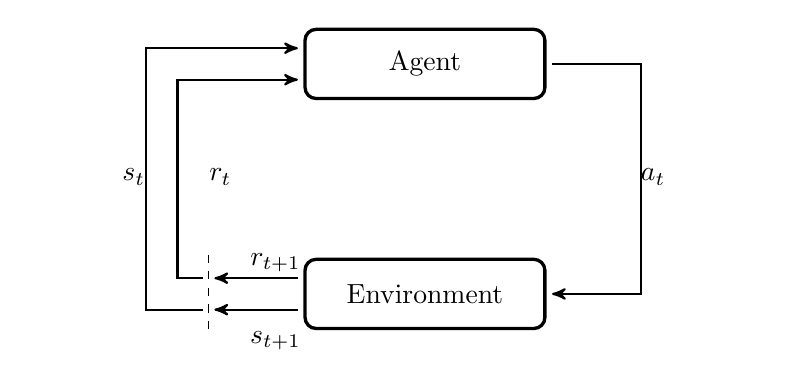
\begin{tikzpicture}
		% node Agent
		\node[punkt] (agent) {Agent};
		% node Environment
		\node[punkt, below=2cm of agent] (env) {Environment};
		% node a_t
		\node[mylabel, below right=0.75cm and 0cm of agent] (action) {$a_t$};
		% node s_t
		\node[mylabel, below left=0.75cm and 0.8cm of agent] (state) {$s_t$};
		% node r_t
		\node[mylabel, below left=0.75cm and -0.3cm of agent] (reward) {$r_t$};
		% node s_t+1
		\node[mylabel, above left=-1.3cm and -1cm of env] (state) {$s_{t+1}$};
		% node r_t+1
		\node[mylabel,above left=-.3cm and -1cm of env] (reward1) {$r_{t+1}$};
		\draw[pil]   (agent.east) -- ($(agent.east) + (1.2cm,0cm)$)  |-  (env.east);
		\draw[pil]   ($(env.west) + (0,-0.2cm)$) -- ($(env.west) + (-1.2cm,-0.2cm)$);
		\draw[pil]   ($(env.west) + (-1.2cm,-0.2cm)$) -- ($(env.west) + (-2cm,-0.2cm)$) |-($(agent.west) + (0,0.2cm)$);
		\draw[pil]   ($(env.west) + (0,+0.2cm)$) -- ($(env.west) + (-1.2cm,+0.2cm)$);
		\draw[pil]   ($(env.west) + (-1.2cm,+0.2cm)$) -- ($(env.west) + (-1.6cm,+0.2cm)$) |-($(agent.west) + (0,-0.2cm)$);
		\draw[dashed]  ($(env.west) - (1.2cm,-0.5cm)$) -- ($(env.west) - (1.2cm,0.5cm)$);
	\end{tikzpicture}
	\caption[Interaction loop between Agent and Environment]{Interaction loop between Agent and Environment. The reward and the state resulting from taking an action become the input of the next iteration. \cite{sutton2018reinforcement}}
	\label{fig:interactionsAE}
\end{figure}
\subsubsection{The Markov decision problem}

With all the definitions shown so far, it is possible to formalise the type of problems on which RL can unleash all its features: the Markov decision process (MDP), a mathematic framework to model decision processes. Its main application fields are optimization and dynamic programming.

A MDP is defined by:
\begin{equation}\label{eq:mdp}
	\begin{gathered}
		<\mathcal{S}, \mathcal{A}, \mathcal{P}, \mathcal{R}, \gamma>\\
		\begin{aligned}
			\text{where}\hspace{10pt} \mathcal{S} & \text{ is a finite set of states}                     \\
			\mathcal{A}                           & \text{ a finite set of actions}                       \\
			\mathcal{P}                           & \text{ a state transition probability matrix}\;\;
			\mathcal{P}_{ss'}^a = \mathbb{P}[s_{t+1}= s' | s_t = s, a_t = a]                              \\
			\mathcal{R}                           & \text{ a reward function}
			\;\; \mathcal{R}_{s}^a = \mathbb{E}[r_{t+1} | s_t = s, a_t = a]                               \\
			\gamma                                & \text{ a discount factor such that } \gamma \in [0,1]
		\end{aligned}
	\end{gathered}
\end{equation}
The main goal of an MDP is to select the best action to take, given a state, in order to collect the best reward achievable.

\subsubsection{Policies, models and value functions} \label{pmvf}
In this quick overview of central units of RL, the components that may compose the agent, the brain of the RL problem can not be missing: they are the \textit{model}, the \textit{policy} and the \textit{value function}.

A \textit{model} consist of information about the environment. These data must not be confused with the ones provided by states and observations: they make it possible to infer prior knowledge about the environment, influencing the behaviour of the agent.

A \textit{policy} is the representation of the agent's behaviour. It is a function that describes the mapping from states to actions.  The policy is represented by $\pi$ and it may be deterministic  $a_t = \pi(s_t)$  or stochastic $\pi(a_t|s_t) = \mathbb{P}[a_t | s_t]$.
In this perspective, it is evident that the central goal of RL is to learn an optimal policy $\pi^*$. The optimal policy is a policy which can show to the agent what the most profitable way to achieve the maximum return is, what is the best action to do in a specific situation. In order to learn the nature of the optimal policy, RL exploits value functions.

A \textit{value function} represents what is the expected reward that the agent can presume to collect in the future, starting from the current state. The reward signal represents only a local value of the reward, while the value function provides a broader view of future rewards: it is a sort of prediction of rewards.
It is possible to delineate two main value functions: the \textit{state value} function and the \textit{action value} function.

\begin{itemize}
	\item The \textit{State Value Function} $V^\pi(s)$ is the expected return starting from the state $s$ and always acting according to policy $\pi$.
	      \begin{equation} \label{eq:statevalue}
		      V^\pi(s) = \mathbb{E}_{\tau \sim \pi}[g_t | s_0 = s]
	      \end{equation}
	\item The \textit{Action Value Function} $Q^\pi(s)$ is the expected return starting from the state $s$, taking an action $a$ and then always acting according to policy $\pi$.
	      \begin{equation} \label{eq:actionvalue}
		      Q^\pi(s, a) = \mathbb{E}_{\tau \sim \pi}[g_t | s_0 = s, a_0 = a]
	      \end{equation}
\end{itemize}


\subsection{Bellman equations}

Both \vref{eq:statevalue,eq:actionvalue} satisfy recursive relationships between the value of a state and the values of its successor states. It is possible to see this property deriving \textit{Bellman equations} \cite{bellman2015applied} -- shown in \vref{eq:bellman} and demonstrated in \vref{appendix:bellmaneq} -- where $s_{t+1}\sim \mathit{E}$ means that the next state is sampled from the environment $E$ and $a_{t+1}\sim \pi$ shows that the policy $\pi$ determines the next action.
\begin{align} \label{eq:bellman}
	\begin{split}
		V^\pi(s_t) &= \mathbb{E}_{a_t \sim \pi, s_{t+1} \sim E}[r(s_t, a_t) + \gamma V^\pi(s_{t+1})] \\
		&= \sum_{a \in \mathcal{A}}\pi(a|s)\sum_{s' \in \mathcal{S}, r \in \mathcal{R}}P(s', r | s, a)\big[r + \gamma V^\pi(s')\big]\\
		Q^\pi(s_t,a_t) &= \mathbb{E}_{s_{t+1} \sim E}[r(s_t, a_t) + \gamma \mathbb{E}_{ a_{t+1} \sim \pi}[Q^\pi(s_{t+1}, a_{t+1})]]\\
		&= \sum_{a \in \mathcal{A}}\pi(a|s)\sum_{s' \in \mathcal{S}, r \in \mathcal{R}}P(s', r | s, a)\big[r + \gamma Q^\pi(s',a')\big]\\
	\end{split}
\end{align}
$r(s_t, a_t)$ is a placeholder function to represent the reward given the starting state and the action taken.
As discussed above, the goal is to find the optimal policy $\pi^*$ to exploit. It can be done using \textit{Bellman optimality equations} defined in \vref{eq:optbellman}.
\begin{align} \label{eq:optbellman}
	\begin{split}
		V^*(s_t) &= \max_{a} \mathbb{E}_{s_{t+1} \sim E}[r(s_t, a) + \gamma V^*(s_{t+1})] \\
		&= \max_{a}\sum_{s' \in \mathcal{S}, r \in \mathcal{R}}P(s', r | s, a)\big[r + \gamma V^*(s')\big]\\
		Q^*(s_t,a_t) &= \mathbb{E}_{s_{t+1} \sim E}[r(s_t, a_t) + \gamma \max_{a'}[Q^*(s_{t+1}, a')]]\\
		&= \sum_{s' \in \mathcal{S}, r \in \mathcal{R}}P(s', r | s, a)\big[r + \gamma \max_{a'} Q^*(s',a')\big]\\
	\end{split}
\end{align}

Therefore, value functions allow defining a partial ordering over policies such that \[\pi \ge \pi' \text{ if } V_\pi \ge V_{\pi'},\forall s \in \mathcal{S}\]
This definition is helpful to enounce the \textit{sanity theorem}. It asserts that for any MDP there exists an optimal policy $\pi^*$ that is better than or equal to all other policies, $\pi^* \ge \pi, \forall \pi$, but also that all optimal policies achieve the optimal state value function and the optimal action-value function.

The solution of the Bellman optimality equation is not linear and, in general, there is no closed-form solution. For this reason, there are many iterative methods: \vref{dp,mfa} contain some of them.


\subsection{Approaches to Reinforcement Learning} \label{approaches}

Every agent consists of an RL algorithm that it exploits to maximise the reward it receives from the environment. Every single algorithm has its singularity, and it could work with a specific application field which depends on the particular approach it supports. Understanding differences among these groups is useful to adequately understand what type of algorithm satisfies better the needs of a specific problem. Nowadays, RL algorithms are numerous, and drawing the complete picture behind them could be a complicated purpose. The distinctions presented in this section aims to describe the most crucial distinctions that are useful in the context of the thesis without claiming to be exhaustive.

\subsubsection{Components of learning}

The first worthy distinction between RL algorithms can be made analysing how the algorithms exploit the different components of the agent: indeed it is possible to explain the main strategies in RL using \textit{policy}, \textit{model} and \textit{value function} defined in \vref{pmvf}.


One of the most crucial aspects of an RL algorithm is the question of whether the agent has access to or learns the model of the environment: this element enables the agent to predict state transitions and rewards.
A method is \textit{model-free} when it does not exploit the model of the environment to solve the problem. All the actions made by the agent results from direct observation of the current situation in which the agent is. It takes the observation, does computations on them and then select the best action to take.
This last representation is in contrast with \textit{model-based} methods. In this case, the agent tries to build a model of the surrounding environment in order to infer information useful to predict what the next observation or reward would be.
Both groups of methods have strong and weak sides.
Ordinarily, \textit{model-based} methods show their potential in a deterministic environment (e.g. board game with rules). In these contexts, the presence of the model enables the agent to plan by reasoning ahead, to recognise what would result from a specific decision before taking action. The agent can extract all this knowledge and learn an optimal policy to follow. However, this opportunity is not always achievable: the model may be partially or entirely unavailable, and the agent would have to learn the model from its experience. Learning a model is radically complex and may lead to various hurdles to overcome: for instance, the agent can exploit the bias present in the model, producing an agent which is not able to generalise in real environments.
On the other hand, model-free methods tend to be more straightforward to train and tune because it is usually hard to build models of a heterogeneous environment. Furthermore, model-free methods are more popular and have been more extensively developed and tested than model-based methods.

The use of policy or value function as the central part of the method represents another essential distinction between RL algorithms.
The approximation of the policy of the agent is the base of \textit{policy-based} methods. The representation of the policy is usually a probability distribution over available actions. This method points to optimise the behaviour of the agent directly and may ask manifold observations from the environment: this fact makes this method not so sample-efficient.
On the opposite side, methods could be \textit{value-based}. In this case, the agent is still involved in finding the optimal behaviour to follow, but indirectly. It is not interested anymore about the probability distribution of actions. Its main objective is to determine the value of all actions available, choosing the best one. The main difference from the policy-based method is that this method can benefit from other sources, such as old policy data or replay buffer.

\begin{figure}
	\centering
	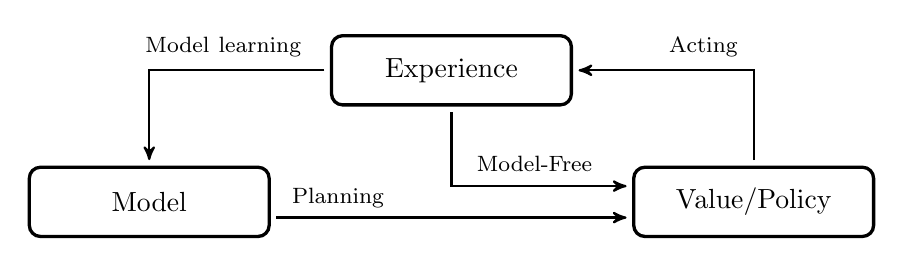
\begin{tikzpicture}
		% node Agent
		\node[punkt] (experience) {Experience};
		% node Environment
		\node[punkt, below left=0.75cm and 0.75cm of experience] (model) {Model};
		% node Value/Policy
		\node[punkt, below right=0.75cm and 0.75cm of experience] (valpol) {Value/Policy};
		\node[mylabel, above left=0.05cm and 0.00cm of experience.west] (ml) {\footnotesize Model learning};
		\node[mylabel, above right=0.05cm and 0.3cm of experience.east] (a) {\footnotesize Acting};
		\node[mylabel, below right=0.5cm and -0.3cm of experience.south] (a) {\footnotesize Model-Free};
		\node[mylabel, above right=-0.2cm and -0.5cm of model.east] (a) {\footnotesize Planning};
		\draw[pil]   (experience.south) -- ($(experience.south) - (0cm,1cm)$)  |-  ($(valpol.west) + (0cm,0.2cm)$);
		\draw[pil]   (experience.west)  -| (model.north);
		\draw[pil]   (valpol.north) -- ($(valpol.north) + (0cm,1cm)$)  |-  (experience.east);
		\draw[pil]   ($(model.east) - (0cm,0.2cm)$)  --  ($(valpol.west) - (0cm,0.2cm)$);
	\end{tikzpicture}
	\caption[Overview of different components in learning]{\small Overview of components of an agent with their relation in respect of different approaches of learning. Model-Free methods works with the experience, value functions and the policy, while model-based techniques tries to build up a model to derive value functions and policy to act in the environment.}
	\label{fig:components}
\end{figure}

\subsubsection{Learning settings}

The learning setting could be \textit{online} or \textit{offline}. In the first case, the learning process is done in parallel or concurrently while the agent continues to gather new information to use, while the second one progresses toward learning using limited data.
Generalisation becomes a critical problem in the latter approach because the agent is not able to interact anymore with the environment.
In the context of this thesis, what matters is \textit{online learning}: the learning phase is not bound to already gathered data, but the whole process goes on using both old data coming from replay buffers and brand new data obtained in the most recent episode.

Another significant difference in RL algorithms consists of the distinctive usage of the policy to learn.
\textit{On-policy} algorithms profoundly depend on the training data sampled according to the current policy because they are designed to use only data gathered with the last learned policy.
On the other hand, an \textit{off-policy} method can use a different source of valuable data for the learning process instead of direct experience. This feature allows the agent to use, for instance, large experience buffers of past episodes. In this context, these buffers are usually randomly sampled in order to make the data closer to being independent and identically distributed (i.i.d): random extraction guarantees this fact.


\subsection{Dynamic programming} \label{dp}

Dynamic programming (DP) is one of the approaches used to resolve RL problems. Formally, it is a general method to explain complex problems by breaking them into more manageable sub-problems. After solving all sub-problems, it is possible to sum them up in order to obtain the final solution to the whole original problem.
This technique provides a practical framework to solve MDP problems and to observe what is the best result achievable from it, but it assumes to have full knowledge about the specific problem. For this reason, it applies primarily to model-based problems.

Furthermore, dynamic programming methods \textit{bootstrap}: it means that these strategies use one or more estimated values in the update step for the same kind of estimated value, leading to results more sensitive to initial values.

\subsubsection{Policy Iteration}

The \textit{policy iteration} aims to find the optimal policy by directly manipulating the starting policy. However, before proceeding with this process, a proper evaluation of the current policy is essential. This procedure can be done iteratively following \vref{policy_evaluation} where $\theta$ is the parameter that defines the accuracy: the more the value is closer to $0$, the more the evaluation would be precise.

\textit{Policy improvement} is the second step towards policy iteration. Intuitively, it is possible to find a more valuable policy than the starting one by changing the action to select in a specific state with a more rewarding one.  The key to check if the new policy is better than the previous one is to use the action-value function $Q_\pi(s,a)$. This function returns the value of taking action $a$ in the current state $s$ and, after that, following the existing policy $\pi$. If $Q_\pi(s,a)$ is higher than $V_\pi(s)$, so the action selected is better than the action chosen by the current policy, and consequently, the new policy would be better overall.

Policy improvement theorem is the formalisation of this fact: \vref{policyimprovement} shows its demonstration. Thanks to this theorem, it is reasonable to act greedily to find a better policy starting from the current one iteratively selecting the action that produces the higher  $Q_\pi(s, a)$ for each state.

%\begin{align}\label{eq:greedy}
%\begin{split}
%\pi'(s) &\doteq \underset{a}{\arg\max\,} Q_\pi(s, a)\\
%		&= \underset{a}{\arg\max\,} \mathbb{E}[r_{t+1}+\gamma V_\pi(s_{t+1})|s_t = s, a_t = a]\\
%		&= \underset{a \in \mathcal{A}}{\arg\max\,} \sum_{s' \in \mathcal{S}, r \in \mathcal{R}}P(s',r |s, a)\bigg[r+\gamma V_\pi(s')\bigg]\\
%\end{split}
%\end{align}

The iterative application of policy improvement stops after an improvement step that does not modify the initial policy, returning the optimal policy found.

\subsubsection{Value Iteration}

The second approach used by dynamic programming to solve Markov decision processes is \textit{value iteration}.
Policy iteration is an iterative technique that alternate evaluation and improvement until it converges to the optimal policy.
On the contrary, value iteration uses a modified version of policy evaluation to determine $V(s)$ and then it calculates the policy.
The pseudocode of this method is available \vref{value_iteration}.

\subsubsection{Generalised Policy Iteration}

Generalised Iteration Policy (GPI) indicates the idea underlying the interaction between evaluation and improvement steps seen in value and policy iteration.
\Vref{fig:gpi} reports how the two processes compete and cooperate to find the optimal value function and an optimal policy. The first step, known as policy evaluation step, exploits the current policy to build an approximation of the value function. The second step, known as policy improvement step, tries to improve the policy starting from the current value function.
This iterative scheme of dynamic programming can represent almost all reinforcement learning algorithm.

\begin{figure}[!h]
	\centering
	\begin{minipage}[b]{0.2\textwidth}
		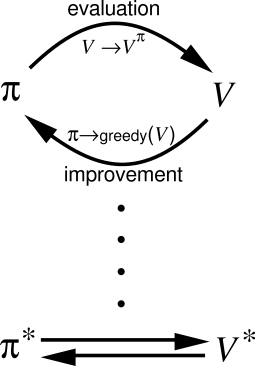
\includegraphics[width=\textwidth]{img/gpi00.png}
	\end{minipage}
	\begin{minipage}[b]{0.5\textwidth}
		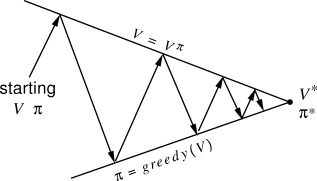
\includegraphics[width=\textwidth]{img/gpi01.png}
	\end{minipage}
	\caption{\small Generalised policy iteration schema \cite{sutton2018reinforcement}. Value and policy functions compete and cooperate to reach the joint solution: the optimal value function and an optimal policy.}
	\label{fig:gpi}
\end{figure}

\subsection{Model-free approach} \label{mfa}

As reported in the previous section, having a comprehensive knowledge of the environment is at the foundation of dynamic programming methods. However, this fact is not always accurate in practice, where it is infrequent to have a full understanding of how the world works. In these cases, the agent has to infer information using its experience, so it has to exploit model-free methods, based on the assumption that there is no prior knowledge about state transitions and rewards.
This section intends to provide a brief description of two model-free approaches to prediction and control: Monte Carlo (MC) methods and Temporal-Difference (TD) ones.

\subsubsection{Monte Carlo learning}

Monte Carlo methods \cite[Chapter 6]{sutton2018reinforcement} can learn from episodes of experience using the simple idea that averaging sample returns provide the value. This lead to the main caveat of these methods: they work only with episodic MDPs because the episode has to terminate before it is possible to calculate any returns.
The total reward accumulated in an episode and the distribution of the visited states is used to calculate the value function while the improvement step is carried out by making the policy greedy concerning the value function.

This approach brings to light the exploration dilemma about how it is possible to guarantee that the algorithm will explore all the states without prior knowledge of the whole environment. $\epsilon$-greedy policies are exploited instead of full greedy policy to solve this problem.
An $\epsilon$-greedy policy is a policy that acts randomly with probability $\epsilon$ and follows the policy learned with probability $(1-\epsilon)$.

Unfortunately, even though Monte Carlo methods are simple to implement and they are unbiased because they do not bootstrap, they require a high number of iteration to converge. Furthermore, they have a wide variance in their value function estimation due to lots of random decisions within an episode.

\subsubsection{Temporal Difference learning} \label{tdlearn}

Temporal Difference (TD) is an approach made combining ideas from both Monte Carlo methods and dynamic programming. TD is a model-free method like MC but uses bootstrapping to make updates as in dynamic programming. The central distinction from MC approaches is that TD methods calculate a \textit{temporal error} instead of using the total accumulated reward. The temporal error is the difference between the new estimate of the value function and the old one. Furthermore, they calculate this error considering the reward received at the current time step and use it to update the value function: this means that these approaches can work with continuing (non-terminating) environments.
This type of update reduces the variance compared to Monte Carlo one but increases the bias in the estimate of the value function because of bootstrapping.

The fundamental update equation for the value function is shown in \vref{eq:tdlearning}, where \textit{TD error} and \textit{TD target} are in evidence.
\begin{equation}\label{eq:tdlearning}
	V(s_t) \leftarrow V(s_t) + \alpha \big(\underbrace{\overbrace{r_{t+1} + \gamma V(s_{t+1})}^{\text{TD target}}- V(s_t)}_{\text{TD error} \ (\delta_t)}\big)
\end{equation}
Two TD algorithms for the control problem which are worth quoting because of their extensive use to solve RL problems are \textit{SARSA (State-Action-Reward-State-Action)} and \textit{Q-Learning}.

\textit{SARSA} is an on-policy temporal difference algorithm whose first step is to learn an action-value function instead of a state-value function. This approach leads to focus not to estimate the specific value of each state, but to determine the value of transitions and state-action pairs. \Vref{eq:sarsa} represents the update function of \textit{SARSA}, while \vref{alg:sarsa} summarise its pseudocode.
\begin{equation}\label{eq:sarsa}
	Q(s_t, a_t) \leftarrow Q(s_t, a_t) + \alpha [r_{t+1} + \gamma Q(s_{t+1}, a_{t+1}) - Q(s_t, a_t)]
\end{equation}
\begin{figure}

	\begin{algorithm}[H]
		\SetAlgoLined
		\DontPrintSemicolon
		\LinesNumbered
		\KwIn{step size $\alpha \in (0,1]$, small $\epsilon > 0$\;}
		Initialise $Q(s,a) \; \forall\; s \in \mathcal{S}, a \in \mathcal{A}$ arbitrarily, except that $Q(\text{terminal}, \cdot) = 0$\;
		\ForEach{episode}{
			Initialise $s_t$ \;
			Choose $a_t$ from $s_t$ using policy derived from $Q$ (e.g.\ $\epsilon$-greedy) 	 \;
			\Repeat{$s_t$ is terminal}{
				Take action $a_t$ $\rightarrow$ obtain $r_{t+1}$ and $s_{t+1}$ \;
				Choose $a_{t+1}$ from $s_{t+1}$ using policy derived from Q (e.g.\ $\epsilon$-greedy) \;
				$Q(s_t, a_t) \leftarrow Q(s_t, a_t) + \alpha [r_{t+1} + \gamma Q(s_{t+1}, a_{t+1}) - Q(s_t, a_t)]$\;
				$s_t \leftarrow s_{t+1}$ ; $a_t \leftarrow a_{t+1}$
			}
		}
		\caption{SARSA (on-policy TD control) for estimating $Q \approx q_*$}
		\label{alg:sarsa}
	\end{algorithm}
\end{figure}

\textit{Q-learning} \cite{watkins1989learning} is an off-policy TD control algorithm which represents one of the early revolution and advance in reinforcement learning.
The main difference from SARSA is the update rule for the Q-function: it selects the action in respect of an $\epsilon$-greedy policy while the Q-function is refreshed using a greedy policy based on the current Q-function using a max function to select the best action to do in the current state with the current policy.
\Vref{eq:qlearning} represents the update function of \textit{Q-learning}, while \vref{alg:qlearning} summarise its pseudocode.
\begin{equation}\label{eq:qlearning}
	Q(s_t, a_t) \leftarrow Q(s_t, a_t) + \alpha [r_{t+1} + \gamma \max_{a}{Q(s_{t+1}, a)} - Q(s_t, a_t)]
\end{equation}
\begin{figure}

	\begin{algorithm}[H]
		\SetAlgoLined
		\DontPrintSemicolon
		\LinesNumbered
		\KwIn{step size $\alpha \in (0,1]$, small $\epsilon > 0$\;}
		Initialise $Q(s,a) \; \forall\; s \in \mathcal{S}, a \in \mathcal{A}$ arbitrarily, except that $Q(\text{terminal}, \cdot) = 0$\;
		\ForEach{episode}{
			Initialise $s_t$ \;
			Choose $a_t$ from $s_t$ using policy derived from $Q$ (e.g.\ $\epsilon$-greedy) 	 \;
			\Repeat{$s_t$ is terminal}{
				Take action $a_t$ $\rightarrow$ obtain $r_{t+1}$ and $s_{t+1}$ \;
				Choose $a_{t+1}$ from $s_{t+1}$ using policy derived from Q (e.g.\ $\epsilon$-greedy) \;
				$Q(s_t, a_t) \leftarrow Q(s_t, a_t) + \alpha [r_{t+1} + \gamma \max_{a}{Q(s_{t+1}, a)} - Q(s_t, a_t)]$\;
				$s_t \leftarrow s_{t+1}$ ; $a_t \leftarrow a_{t+1}$
			}
		}
		\caption{Q-learning (off-policy TD control) for estimating $\pi \approx \pi_*$}
		\label{alg:qlearning}
	\end{algorithm}
\end{figure}

\subsubsection{Temporal Difference Lambda Learning}

As reported previously, Monte Carlo and Temporal Difference learning perform updates in different ways. The first approach exploits the total reward to update the value function, while the second one, on the other hand, works with the reward of the current step. Temporal Difference Lambda, also known as TD($\lambda$) \cite[Chapter 7,12]{sutton2018reinforcement}, represents a combination of these two procedures and it takes into account the results of each time step together with the weighted average of those returns.
The idea of calculating TD target looking n-steps into the future instead of considering only a single step is the baseline of TD($\lambda$). This lead to the formalisation of the $\lambda$-weighted return $G_t^\lambda$ presented in \vref{eq:lambdaG}.
\begin{equation}\label{eq:lambdaG}
	G_t^\lambda = (1-\lambda)\sum_{n=1}^{\infty}\lambda^{n-1}G_t^{(n)}
\end{equation}
TD($\lambda$) implementation takes into account an additional variable called eligibility trace $e_t(s_t)$ which indicates how much learning should be carried out for each state for each timestep. It aims to describe how much the agent encountered a specific state recently and \vref{eq:eligibility_trace} describes the updating rule of this value where the $\lambda$ represents the trace-decay parameter.
\begin{equation}\label{eq:eligibility_trace}
	e_t(s) = \gamma \lambda e_{t-1}(s) + \mathbbm{1}(s = s_t)
\end{equation}

\subsection{Model-based approach}


Heretofore, the focus of this section was on methods which have no prior knowledge of the environment, since this thesis grows on model-free foundations.
Despite this point, it is worth to summarise the main concepts behind model-based approaches.
Model-based methods gather information to enable the ability of planning, which can enhance the sample efficiency of the algorithm.

There are two primary principles to model-based learning. The first one implies to assemble a model starting from prior knowledge and to exploit it to calculate the policy and the value-function, while the second one is to infer the model from the environment by sampling experience.
The central drawback of the first technique is that prior knowledge could be not as accurate as expected, leading to sub-optimal results. Consequently, the preferred way to learn is the second one.

The decisive point behind these approaches is that they are more sample-efficient concerning model-free ones: they require fewer data to learn a policy. On the other hand, the algorithm must learn the policy as well as the model: this translates to two different sources of approximation errors and an increase of computational complexity.

\section{Deep reinforcement learning} \label{deepreinflearn}

%\todomacaluso{
%	\begin{itemize}
%		\item Introduction and motivation behind function approximation
%		\item Value-based methods and Policy Gradient methods
%		\item Focus and detailed description of DDPG and SAC
%	\end{itemize}	
%}


The strategies shown so far works smoothly with systems with well-defined states and actions. In this context, it is reasonable to use lookup tables to describe the problem: state-value function V has an entry for each state while in action-value function Q has an entry for each state-action pair.
It is easy to understand how this setting cannot scale up with very large MDPs: problems regarding the availability of memory arise as it becomes difficult to manage the storage of a large number of states and actions. Also, there may be obstacles concerning the slowness of learning the value of each state individually. Furthermore, the tabular form could lead to expensive computation in linear lookup and can not work with continuous action and state space.

Function approximators represent the solution to overwhelm this problem. The underlying intention is to use a vector $\theta = (\theta_1, \theta_2. \dots, \theta_n)^T$ to estimate state-value and action-value function as shown in \vref{eq:fun_appr}, generalise from seen states to unseen states and finally update parameter $\theta$ using MC or TD Learning strategies.
\begin{equation}\label{eq:fun_appr}
	\begin{aligned}
		V(s, \theta)    & \approx V_\pi(s)   \\
		Q(s, a, \theta) & \approx Q_\pi(s,a)
	\end{aligned}
\end{equation}
In these terms, function approximators can be considered as a mapping from the vector $\theta$ to the value function.
This choice leads to a reduction in the number of parameters to learn and consequently to a system which can generalise better in fewer training samples.

Nowadays, since its widespread use in research, neural networks represent the most intuitive option to take as function approximator: it reduces the training time for high dimensional systems, and it requires less space in memory.
This point represents the bridge between traditional reinforcement learning and recent discoveries in the theory of deep learning.
Thanks to the last decade great fervour of deep learning, neural networks have become the fundamental tool to exploit as function approximator to develop deep reinforcement learning (Deep RL) which accomplished remarkable results. One of the first steps towards Deep RL and general artificial intelligence -- an AI broadly applicable to a different set of various environments -- was done by DeepMind with their pioneering paper \cite{mnih2013playing} and the consequent \cite{mnih2015human}.

Because of the nature of this work, the focus of this section will be on model-free algorithms.
This section aims to explain the state-of-the-art and the leading theory behind Deep RL framework together with an overview about deep learning and to define two deep actor-critic algorithms used in the experiments of this thesis: Deep Deterministic Policy Gradient (DDPG) and Soft Actor-Critic (SAC).

\subsection{Fundamentals of Deep Learning}

\subsubsection{Artificial Neural Networks}
Deep learning (DL) is an approach to learning based on a function $f: \mathcal{X} \rightarrow \mathcal{Y}$ parametrised with $w \in \mathbb{R}^{n_w} (n_w \in \mathbb{N})$ such that $y = f(x;w)$.

The starting point of this research field is the artificial neuron, inspired by the biological neuron from the brain of animals and human being. A neuron consists of numerous inputs called \textit{dendrites} coming from preceding neurons. Therefore, the neuron elaborates the input and, only if the value reaches a specific potential, it \textit{fires} through its single output called \textit{axon}.

The neuron elaborates the inputs by taking the weighted sum, adding a bias $b$ and applying an activation function $f$ following the relation $y = f( \sum_{n}w x_i + b)$. \Vref{fig:neuron} shows the parallel comparison between the biological neuron and the artificial one. The set of parameter $w$ needs to be adjusted to find a good parameter set: this process is called \textit{learning}.
\begin{figure}[!h]
	\centering
	\begin{minipage}[b]{0.5\textwidth}
		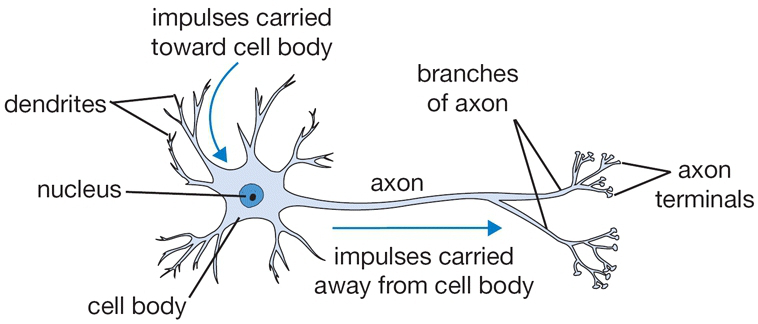
\includegraphics[width=\textwidth]{img/neuron.png}
	\end{minipage}
	\begin{minipage}[b]{0.4\textwidth}
		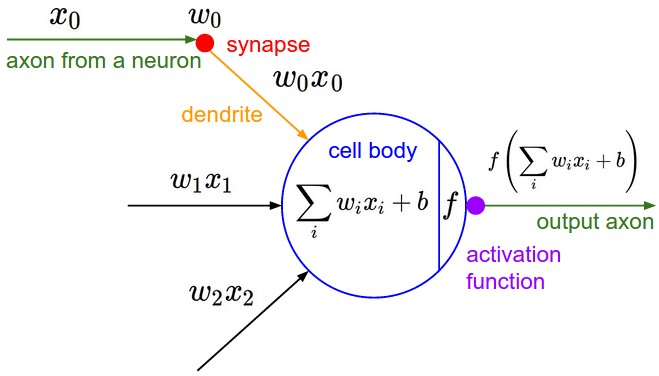
\includegraphics[width=\textwidth]{img/neuron_model.jpeg}
	\end{minipage}
	\caption{\small Comparison between biological neuron (left) and artificial neuron (right). The artificial neuron designs the dendrites as weighted inputs and returns the sum through an activation function. \cite{stanford2019cs231n}.}
	\label{fig:neuron}
\end{figure}

A deep neural network (NN) organises a set of artificial neurons in a series of processing layers to which correspond non-linear transformation.
The whole sequence of these alterations directs the learning process through different levels of abstraction \cite{erhan2009visualizing}.
To better understand the nature of a deep neural network, it is convenient to describe a neural network with one fully-connected layer represented by \vref{fig:fullyconnected}.
\begin{equation}\label{eq:non_linear_transformation}
	\begin{gathered}
		h = g(w_1 \cdot i + b_1) \\
		o = w_2 \cdot h + b_2
	\end{gathered}
\end{equation}
\begin{figure}
	\centering
	\tikzset{%
		every neuron/.style={
				circle,
				draw,
				minimum size=1cm
			},
		neuron missing/.style={
				draw=none,
				scale=4,
				text height=0.333cm,
				execute at begin node=\color{black}$\vdots$
			},
	}
	\resizebox{0.5\textwidth}{!}{
		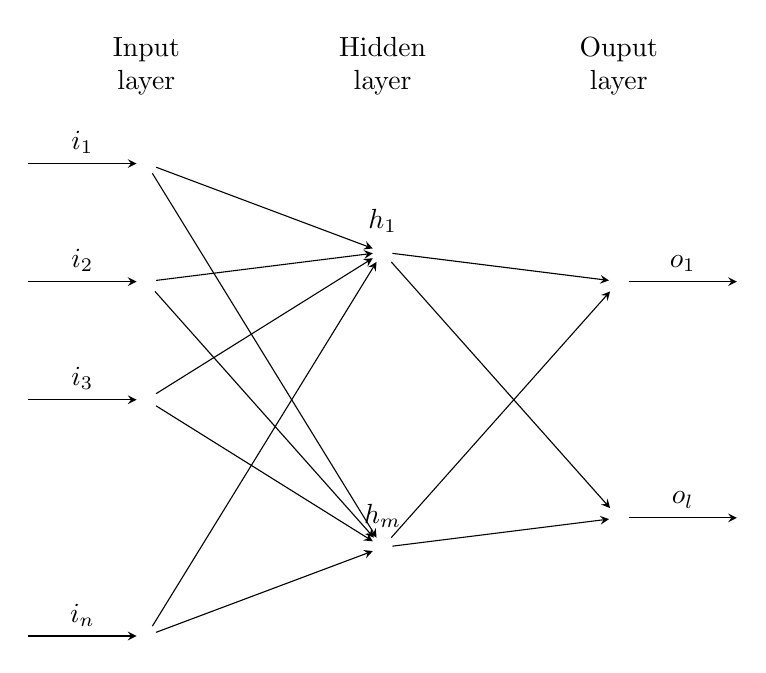
\begin{tikzpicture}[x=1.5cm, y=1.5cm, >=stealth]

			\foreach \m/\l [count=\y] in {1,2,3,missing,4}
			\node [every neuron/.try, neuron \m/.try] (input-\m) at (0,2.5-\y) {};

			\foreach \m [count=\y] in {1,missing,2}
			\node [every neuron/.try, neuron \m/.try ] (hidden-\m) at (2,2-\y*1.25) {};

			\foreach \m [count=\y] in {1,missing,2}
			\node [every neuron/.try, neuron \m/.try ] (output-\m) at (4,1.5-\y) {};

			\foreach \l [count=\i] in {1,2,3,n}
			\draw [<-] (input-\i) -- ++(-1,0)
			node [above, midway] {$i_\l$};

			\foreach \l [count=\i] in {1,m}
			\node [above] at (hidden-\i.north) {$h_\l$};

			\foreach \l [count=\i] in {1,l}
			\draw [->] (output-\i) -- ++(1,0)
			node [above, midway] {$o_\l$};

			\foreach \i in {1,...,4}
			\foreach \j in {1,...,2}
			\draw [->] (input-\i) -- (hidden-\j);

			\foreach \i in {1,...,2}
			\foreach \j in {1,...,2}
			\draw [->] (hidden-\i) -- (output-\j);

			\foreach \l [count=\x from 0] in {Input, Hidden, Ouput}
			\node [align=center, above] at (\x*2,2) {\l \\ layer};

		\end{tikzpicture}
	}
	\caption{An example representation of a deep neural network with one fully-connected hidden layer.}
	\label{fig:fullyconnected}
\end{figure}
The input layer receives as input a column vector of input-features $i$ of size $n \in \mathbb{N}$. Every value of the hidden-layer represented by a vector $h$ of size $m \in \mathbb{N}$ is the result of a transformation of the input values given by \vref{eq:non_linear_transformation} where $w_1$ is a matrix of size $m \times n$ and $b_1$ is a bias term of size $m$. $g$ is a non-linear parametric function called activation function, which represents the core of neural networks. Subsequently, the second and last transformation manipulates the hidden layer $h$ to produce the values of the output layer following \vref{eq:non_linear_transformation} using $w_2$ with size $o \times m$ and $b_2$ with size $o$.

\subsubsection{Learning process}

The learning process aims to seek a set of parameters $\theta$ that results in the best possible function approximation for a specific objective. In supervised learning, the actual output $Y$ is available for each particular input $X$, and it is used to update the parameters. The learning process can be carried out iteratively according to the following steps.

\paragraph{Forward pass} The input $X$ is forwarded through the neural network and the output $Y_{pred} = f(X, \theta)$ is gathered.

\paragraph{Loss} The resulting predicted value $Y_{pred}$ is compared with the actual value $Y$ computing the loss function $L(\theta)$. There are a lot of loss functions available to satisfy the particular needs of specific learning tasks. The \textit{error} is the difference between the output of the neural network for a specific input data and the actual value: it is essential to calculate the loss function. One of the most exploited loss function is the \textit{Mean-Squared Error} (MSE) \cite{shalev2014understanding} shown in \vref{eq:backprop} which works with L2-distance.

\begin{equation}\label{eq:backprop}
	\begin{aligned}
		L(y, \hat{y}) = (y_\theta - y)^2 \\
		J = \frac{1}{n}\sum_{i=1}^{n}L(y_i, f(x_i))
	\end{aligned}
\end{equation}

\paragraph{Backpropagation}
The next step is the computation of the global gradient of the loss function $\nabla L(\theta)$, which is carried out together with its backpropagation through the network. The backpropagation algorithm \cite{rumelhart1988learning} calculates the local gradient of loss for each neuron in the hidden layers. The concept underlying this procedure and shown in \vref{eq:chainrule} is the \textit{chain rule} \cite{lecun2015deep}, which computes derivatives of composed functions by multiplying local derivatives.
\begin{equation}\label{eq:chainrule}
	\begin{gathered}
		y = g(x), \;\;\; z = f(g(x)),  \;\;\;
		\frac{\partial z}{\partial x} = \frac{\partial z}{\partial y} \frac{\partial y}{\partial x}
	\end{gathered}
\end{equation}
Therefore, the chain rule is exploited to propagate the calculated global gradient loss $\frac{\partial L(\theta)}{\partial \theta}$ back through the network, in the opposite direction of the forward pass.
The procedure calculates the local derivatives during the forward pass, while estimates the local gradient of loss during backpropagation determining the multiplication between the local derivative and the local gradient of the loss of the connected neuron of the next layer: if the neuron has multiple connections neurons, the algorithms adds up all the gradients.

\paragraph{Update} In this final step consists in the update of the weights of all neurons. There are many ways developed through the years to carry out the update phase, but the most common one is the gradient descent.
The objective of the gradient descent is to minimise the loss function by refreshing the internal parameters of the network in the negative direction of the gradient loss: this choice leads the function approximation process closer to the minimum at each iteration. \Vref{eq:update} describes the update rule presented by the gradient descent where $\alpha$ is the learning rate. The last-mentioned parameter determines how quickly the algorithm should approach the minimum. A higher learning rate leads to a more significant step towards the minimum, which threatens to overshoot the target.
\begin{equation}\label{eq:update}
	\theta \leftarrow \theta -\alpha \nabla_\theta J
\end{equation}
Nowadays, the technique applied in the majority of research projects is stochastic gradient descent which combines batch learning \cite{stanford2019cs231n} and gradient descent, but also its various improved extensions and variants, such as ADAM \cite{kingma2014adam} and AdaGrad \cite{duchi2011adaptive}: these extensions manage to improve the convergence of SGD thanks to the introduction of adaptive learning rates.

\subsubsection{Regularization}

The final aim of the learning process is to obtain a function approximator capable of generalising over data. This fact means that a neural network should show performances on unseen data comparable to the one obtained from training data. For this reason, it is necessary an appropriate trade-off between underfitting and overfitting.

A shallow approximated function and insufficient training data with a lack of diversity are the leading cause to the first situation: the network generalises on the data, but the prediction error is always too high for all data points.
The phenomenon of overfitting describes the exact contrary of underfitting. The leading cause is too complex approximation function: this lead to a network which scores an excellent performance on training data, but poorly predicts unseen points.

Regularisation \cite{bishop2006pattern,lecun2015deep} represents an approach to overcome and prevent the problem of overfitting. It works extending the loss function with a regularised term $\Omega(\theta)$ as shown in \vref{eq:generalreg} where $\lambda$ is the regularisation factor.
\begin{equation}\label{eq:generalreg}
	L'(\theta) = L(\theta, Y, Y_{pred}) + \lambda \Omega(\theta)
\end{equation}
\Vref{eq:l2reg,eq:l1reg} show two examples of regularisation terms. The first is $L^2$-regularisation which exploits the squared sum of the weights $\theta$ in order to keep the weights small. The second approach is known as $L^1$-regularisation: in this case, large weights are less penalised, but this method leads to a sparser solution.
\begin{equation}\label{eq:l2reg}
	L'(\theta) = L(\theta, Y, Y_{pred}) + \lambda \frac{1}{2}||\theta||^2
\end{equation}
\begin{equation}\label{eq:l1reg}
	L'(\theta) = L(\theta, Y, Y_{pred}) + \lambda \frac{1}{2}||\theta||
\end{equation}


\subsubsection{Activation function}

\Vref{eq:activation} shows the most common activation functions: in general, \textit{ReLu}  achieves better performance over a wide variety of tasks, but usually the selection of the best activation function has to be done starting from all information and requirements of the deep learning model.
\begin{equation}\label{eq:activation}
	\begin{aligned}
		\text{Sigmoid} \;\rightarrow\;                      & g(x) = \frac{1}{1+ e^{-x}}           \\
		\text{Hyperbolic Tangent} \;\rightarrow\;           & g(x) = \frac{e^x-e^{-x}}{e^x+e^{-x}} \\
		\text{Rectified Linear Unit (ReLu)} \;\rightarrow\; & g(x) = \max(0,x)
	\end{aligned}
\end{equation}

\subsubsection{Batch Learning and Normalization}
The basic concept underlying \textit{batch learning} \cite{stanford2019cs231n} is to process a set of $n$ training samples called also \textit{mini-batches} in the place of a single one. This method works with the gradient averaged over all the samples in the mini-batch: it leads to a more accurate gradient reducing its variance and the training time.

\textit{Batch normalisation} consists of zero-centring and rescaling all data in a specific batch, resulting in a  mean of normalised data close to $0$ and a variance close to $1$. The algorithm presented in \vref{alg:batchnorm} is the one provided in \cite{ioffe2015batch}.
This method computes the mean $\mu_\beta$ and the variance $\sigma_\beta$  element-wise for each spatial position in the batch: $\epsilon > 0$ is a small value to avoid the division by zero.
The batch normalisation layer then processes the resulting normalised value: $\gamma$ and $\beta$ are the parameters of this layer that are in addition to the original parameter set $\theta$ of the Neural Network in the learning process.
The new learning dynamic provided by the addition of this class of layer increases the network expressivity: applying this method to the input data and the output of any hidden layer results in the reduction of the training time, better regularisation during learning and the reduction of the overfitting phenomenon.
\begin{figure}
	\begin{algorithm}[H]
		\SetAlgoLined
		\setstretch{1.35}
		\DontPrintSemicolon
		\LinesNumbered
		\KwIn{Mini-batch $\mathcal{B} = {x_{1 \dots m}}$; $\gamma$ and $\beta$ prameters to be learned\;}
		\KwOut{$y_i = \text{BN}_{\gamma, \beta}(x_i)$}
		$\mu_\beta \leftarrow \frac{1}{m} \sum_{i=1}^{m} x_i $ \tcp*{Mini-batch mean}
		$\sigma_\beta^2 \leftarrow \frac{1}{m} \sum_{i=1}^{m} (x_i-\mu_\beta)^2 $ \tcp*{Mini-batch variance}
		$\hat{x_i} \leftarrow \frac{x_i - \mu_\beta}{\sqrt{\sigma^2_\beta + \epsilon}} $\tcp*{Normalisation}
		$y_i \leftarrow \gamma \hat{x_i} + \beta \equiv \text{BN}_{\gamma, \beta}(x_i)$\tcp*{Scale and shift}
		\caption{Batch normalisation}
		\label{alg:batchnorm}
	\end{algorithm}
\end{figure}

\subsubsection{Convolutional Neural Networks}

Sensory reception represents how humans and animals react to changes: it consists of sensors which process the input data and are sensitive to specific stimuli.
This system inspires the architecture underlying Convolutional Neural Networks: they could handle efficiently significant input data with many applications in computer vision.
\Vref{fig:lenet5} displays the \textit{LeNet-5} \cite{lecun1998gradient} which is capable to recognise digits in images. It represents a perfect example of a standard convolutional neural network architecture: it consists of a series of convolutional layers followed by a subsampling pooling layer.
At the end of the convolutional stack, the values map into final hidden layers of the network to compute the final low-dimensional output of the network: fully-connected layers usually compose these final layers.
It is possible to suppose that the first layers have to learn low-level features of the input data while succeeding layers are responsible for combining the last-mentioned features in high-level ones.

\begin{figure}[!h]
	\centering
	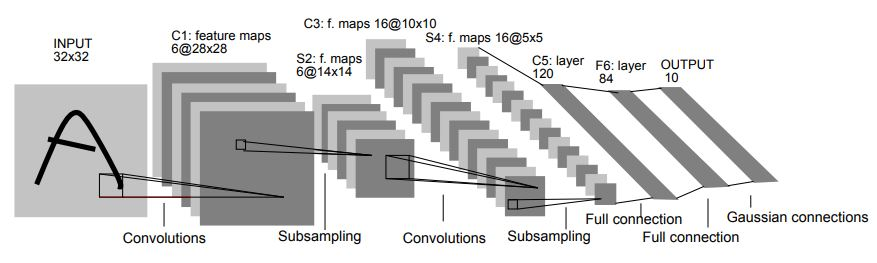
\includegraphics[width=\textwidth]{img/lenet5.jpg}

	\caption{\small Comparison between biological neuron (left) and artificial neuron (right). The artificial neuron designs the dendrites as weighted inputs and returns the sum through an activation function. \cite{stanford2019cs231n}.}
	\label{fig:lenet5}
\end{figure}

\paragraph{Convolutional Layer}

Convolutional layers \cite{lecun1995convolutional} operates with a set of learnable filters (called kernels) with dimensions $n \times m$ smaller than the whole input image. The convolution is the basic operation employed in these class of layer: it consists in convolving each filter across the width and height of the input data and computing dot products between the values in the filter and the ones in the input at any position. The result of this operation is a 2-dimensional activation map that contains the results of that filter at every spatial position.  In this context, the network can learn filters that detect specific features in the image such as edges, textures and patterns \cite{erhan2009visualizing}.

It is possible to compute the output size $W_2 \times H_2 \times D_2$ of a pooling layer using starting from the input size $W_1 \times H_1 \times D_1$ and from the hyperparameters of this class of layer: the number of filters $K$, their spatial extent $F$, the stride $S$ and the amount of zero padding $P$. The resulting volume size can be calculated using the relations reported in \vref{eq:conv}.
\begin{equation} \label{eq:conv}
	\begin{aligned}
		W_2 & = (W_1 - F + 2P)/S + 1 \\
		H_2 & = (H_1 - F + 2P)/S + 1 \\
		D_2 & = K
	\end{aligned}
\end{equation}
The number of parameters introduced by a single kernel is equal to $F \cdot F \cdot D_1$, so the convolutional layer has a total of $(F \cdot F \cdot D_1) \cdot K$ weights and $K$ bias.

In a convolutional layer, the number of weights is kept small and then the computation is more efficient than the one of a fully-connected layer: small filters need fewer parameters and less work in the convolutional operation. Besides this motivation, the filters are kept small also because it makes them capable of learning small and low-level features. The great innovation behind convolutional layers is that the same neuron can recognise the related learned features even if they emerge in different locations of the image: this is the property of translation invariance of feature detection with convolutional layers.


\paragraph{Pooling Layer}

It is common to insert a pooling layer in-between successive convolutional layers. The main objective of this class of layers is to apply a downsampling filter on the input: it progressively reduces the spatial size of the representation, decreasing the number of parameters and the computational cost in the network. It is also useful to control overfitting.

It is possible to compute the size of the output $W_2 \times H_2 \times D_2$ of a pooling layer using starting from the size of the input $W_1 \times H_1 \times D_1$ and from the hyperparameters of this class of layer: the spatial extent of the filter $F$, the stride $S$. The resulting volume size can be calculated using the relations reported in \vref{eq:pool}.
\begin{equation} \label{eq:pool}
	\begin{aligned}
		W_2 & = (W_1 - F)/S + 1  \\
		H_2 & = (H_1 - F )/S + 1 \\
		D_2 & = D_1
	\end{aligned}
\end{equation}
The most common types of pooling layer are the \textit{max-pooling} and the \textit{average-pooling} layer. Both classes return a single value for each position of the filter: the first returns the maximum value, while the second returns the average among the values in the specific section of the input.



\begin{figure}[!h]
	\centering
	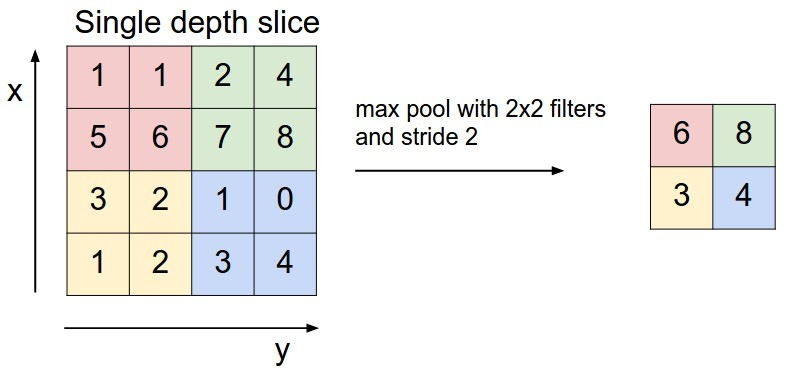
\includegraphics[width=0.7\textwidth]{img/maxpool.jpeg}
	\caption{\small Example of a max-pooling operation with a stride of 2 and a spatial extent of 2. \cite{stanford2019cs231n}.}
	\label{fig:avgpool}
\end{figure}

It is worthy of using a pooling layer in a situation where the exact feature position is not relevant but rather whether a particular feature exists in the input at all.


\subsection{Value-based methods}

The first class of algorithms to explore is value-based one. They works learning an approximator $Q_\theta(s,a)$ to infer the optimal action-value function $Q^*(s,a)$ using an objective function based on Bellman equations.
The preponderance of optimisations belonging to this category is \textit{off-policy}: this means that the optimisation step is done using all data collected during the whole training, not only with the most recent policy available. In this configuration, the information used for the learning phase could also come from exploration decision, apart from ones obtained with the most recent policy.
Indeed, value-based approaches are more sample efficient because they can reuse data more efficiently, but they are considered less stable than policy gradient ones.
Thanks to the relation expressed by $a(s) = \operatornamewithlimits{argmax}_a Q_\theta(s,a)$, it is possible to obtain the policy learned so far from the current action-value function.

\subsubsection{Deep Q-Network (DQN)}
This algorithm grows from the ideas underlying Q-Learning \cite{watkins1989learning}  shown previously in \vref{tdlearn}. The team of DeepMind introduced the Deep Q-Network (DQN) in \cite{mnih2013playing} and in the next cutting-edge paper \cite{mnih2015human}: they managed to create an algorithm capable of learning to play ATARI video-games online using raw image and pixels. It works with neural networks as a function approximator, employing convolutional layers in the first layers of the neural network and performing the optimisation with a variant of stochastic gradient descent called RMSprop \cite{tieleman2012lecture}. The exploited neural network provides as output a probability distribution over all possible discrete actions to determine what is the best action to take.

To overcome the instability problem of value-based methods, DQN utilises two heuristics to narrow instabilities.

\paragraph{Target Network}
The presence of a second network, also called  \textit{target network}, enriches the update phase of this algorithm. \Vref{eq:lossdqn}
defines the loss function of DQN where $y_i$ value is computed using the target network instead of the local network. Therefore, the parameters of the target network are hard updated every $I \in \mathbb{N}$ iterations: this choice precludes instabilities and avoids divergence because of target networks parameters remain fixed for $I$ iterations.
\begin{equation} \label{eq:lossdqn}
	\begin{gathered}
		L_i(\theta_i) = \mathbb{E}_{s, a \sim \pi}\big[(y_i - Q(s, a; \theta_i))^2\big]\\
		y_i = \mathbb{E}_{s' \sim E}[r + \gamma \max_{a'}Q(s',a'; \theta_{i-1})|s,a]
	\end{gathered}
\end{equation}

\paragraph{Experience Memory Replay} \label{experience}

Another crucial introduction in this algorithm is \textit{experience memory replay buffer} \cite{lin1992self}. Trajectories sampled from the environment are temporally correlated, and this could lead to overfitting the parameters of the neural network because the data are not independent and identically distributed (\textit{i.i.d.}). The setting of this algorithm is \textit{online} because the replay buffer stores $N_{\text{replay}} \in \mathbb{N}$ replacing old steps as new ones arrive. The experience is collected as tuples $(s_t,a_t,r_t,s_{t+1})$ using the $\epsilon$-greedy policy. The learning phase samples a set of limited tuples called \textit{mini-batch} allowing a wider set of state-action pair in the update of the network and improving the procedure in terms of variance in respect of single tuple update.
Trajectories sampled from the environment are temporally correlated, and this could lead to overfitting the parameters of the neural network. Using a batch sample from the replay buffer makes the data \textit{i.i.d.} and consequently improves the learning.

\subsubsection{Improvements of DQN}
Further investigation and speculation followed the publication of the thriving DQN. Summing up and comparing these new approaches to original DQN is the main aim of \textit{Rainbow} \cite{hessel2018rainbow}: it also introduces an algorithm called \textit{Rainbow DQN} with all the techniques proposed. The following paragraphs will delineate three main improvements of DQN.

\paragraph{Double DQN}
The double DQN \cite{hasselt2010double, van2016deep} improvement can handle the intricacy of overestimation of Q-values caused by the maximisation step in \vref{eq:lossdqn}. It works with two separate Q-Network with parameters $\theta$ and $\theta^-$ for estimating TD-target. It allows for removing the positive bias in estimating action values, leading to less overestimation of Q-learning values, improved stability and performance. In this context, the target $y_i$ is replaced by \vref{eq:ddqny}.
\begin{equation} \label{eq:ddqny}
	y_i = \mathbb{E}_{s' \sim E}[r + \gamma Q(s',\operatornamewithlimits{argmax}_aQ(s', a; \theta_{i-1}); \theta^-_{i-1})|s,a]
\end{equation}
\paragraph{Prioritised Experience Replay}

The fundamental idea underlying \textit{prioritised experience replay} \cite{schaul2015prioritized} is precisely to prioritise experiences that contain more crucial information than other ones. An additional value that defines the priority of a specific transition joins each tuple stored in the replay buffer: thanks to this approach, experiences with higher priority has a higher sampling probability and are more likely to remain longer in the replay buffer. It is possible to use \textit{TD-error} to measure the importance of each tuple in the experience. A high TD-error means that the agent behaved better or worse than expected in that particular moment, and therefore, it can learn more from that specific passage.

\paragraph{Dueling DQN}

The dueling DQN architecture \cite{wang2015dueling} presented in \vref{fig:duelingdqn} works decoupling the Q-value estimation in two distinct sequences of fully-connected layers right after convolutional layers.
\begin{figure}
	\centering
	\resizebox{0.6\textwidth}{!}{
		\begin{tikzpicture}
			\node at (0,0) (image) {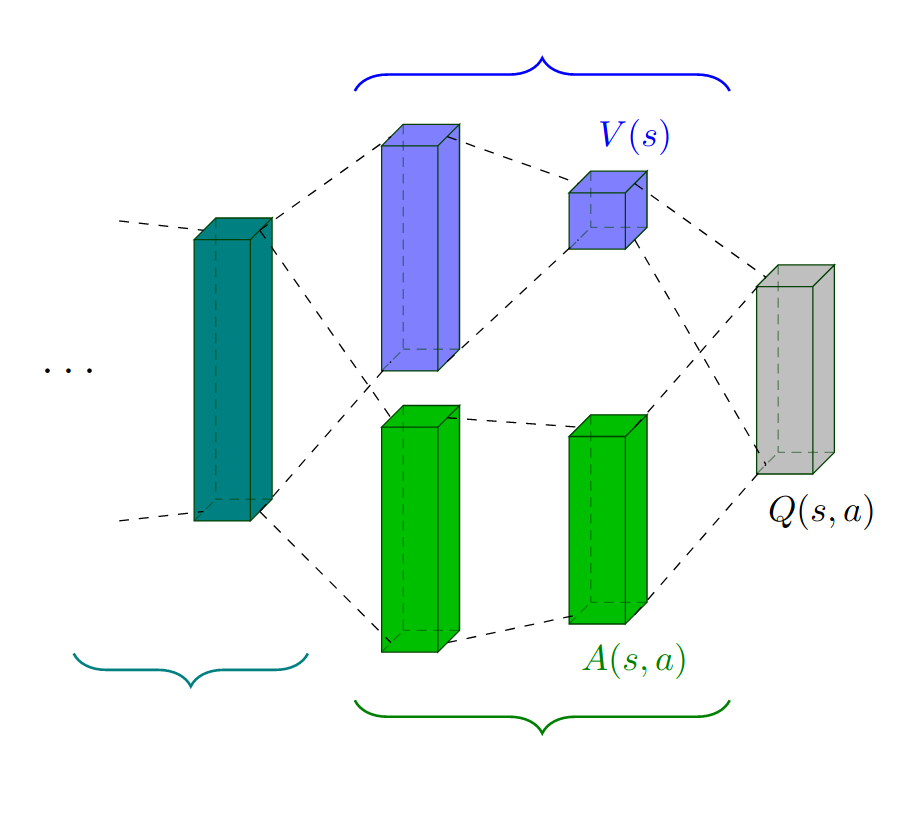
\includegraphics[width=0.7\textwidth]{img/duelingdqnn.png}};
			% node a_t
			\node[mylabel, below right=-0.1cm and -0.5cm of image.north] (action) {\LARGE \textcolor{Blue}{$\beta$}};
			\node[mylabel, above right=0.3cm and -0.5cm of image.south] (action) {\LARGE \textcolor{OliveGreen}{$\alpha$}};
			\node[mylabel, above right=0.8cm and -4.6cm of image.south] (action) {\LARGE \textcolor{PineGreen}{$\theta$}};% node s_t
		\end{tikzpicture}
	}
	\caption[Dueling DQN]{\small Dueling DQN architecture \cite{wang2015dueling}: It consists in two stream to estimate state-value parametrised with $\beta$ and advantages values parametrised with $\alpha$ for each action. The last layer represent the combination of these two types of values to obtain the Q-function. \cite{franccois2018introduction}}
	\label{fig:duelingdqn}
\end{figure}

These streams are capable of providing separate estimates of the state-value  $V(s; \theta, \beta)$ and advantage $A(s,a; \theta, \alpha)$ functions exploited in the end to obtain the Q-value function $Q(s,a; \theta, \alpha, \beta)$ estimate where $\theta$ represents the parameters of convolutional layers while $\alpha$ and $\beta$ the ones of state-value and advantage function respectively.

The first formalisation of the Q-value function is shown by \vref{eq:qvalueddqn0}, but \cite{wang2015dueling} also suggests a different approach shown in \vref{eq:qvalueddqn1} with increased stability in practice.
\begin{gather}
	Q(s,a; \theta, \alpha, \beta) = V(s;\theta, \beta) + \big(A(s,a;\theta, \alpha) - \max_{a' \in \mathcal{A}}A(s, a'; \theta, \alpha)\big) \label{eq:qvalueddqn0}\\
	Q(s,a; \theta, \alpha, \beta) = V(s;\theta, \beta) + \big(A(s,a;\theta, \alpha) - \frac{1}{|\mathcal{A}|}\sum_{a' \in \mathcal{A}}A(s, a'; \theta, \alpha)\big) \label{eq:qvalueddqn1}
\end{gather}



\subsection{Policy gradient methods}

Policy gradient algorithms aim to optimise the policy's performance measure in \vref{eq:pgperf} by finding a suitable policy $\pi_\theta(s|a)$ capable of generating a trajectory $\tau$ that maximises the expected rewards \vref{eq:pgmax} instead of learning a  value function. Indeed the objective function in policy gradient methods consists of maximising $J(\theta)$ value by finding a proper policy updating $\theta$ parameters directly.
\begin{gather}
	J(\theta) = \mathbb{E}\big[\sum_{t=0}^{N}r(s_t,a_t); \pi_\theta\big] = \sum_{\tau}P(\tau;\theta)r(\tau) \label{eq:pgperf}\\
	\theta^* = \operatornamewithlimits{argmax}_\theta J(\theta) \label{eq:pgmax}
\end{gather}
Stochastic gradient ascent is used to refresh the parameters of the policy $\theta$. Gradient ascent is the inverse of gradient descent and updates the parameters $\theta_t$ in the positive direction of the gradient of the policy’s performance measure $\nabla_\theta J(\theta)$ following \vref{eq:pgascent} where $\alpha$ is the learning rate which defines the strength of the steps in the direction of the gradient.
\begin{equation}
	\theta_{t+1} \leftarrow \theta_t + \alpha \nabla_\theta J(\theta_t) \label{eq:pgascent}
\end{equation}
The main advantage of policy gradient approaches consists in the stability of their convergence: these methods work updating their policy directly at each time step instead of renewing value function from which to derive the policy like value-based methods. Last-mentioned approaches can lead to a radical change in the policy output even for a small change in the value function: this event can cause prominent oscillation during training.
Furthermore, policy gradient algorithms can face infinite and continuous action space because the agent estimates the action directly instead of calculating the Q-value for each possible discrete action.
The third feature is their ability to learn stochastic policies, useful in uncertain contexts or partially observable environments.
Despite the presence of the advantages just mentioned, policy gradient methods have an substantial disadvantage: they tend to converge to a local maximum instead of the global optimum.

\subsubsection{Actor-Critic Architecture}

Actor-critic architecture, shown in \vref{fig:actorcritic}, represents the point of contact between value-based approaches and policy gradient methods. They are policy gradient methods basically but exploit value-function to learn the parameters $\theta$ of the policy. As its name suggests, these approaches work with two different parts called \textit{actor} and \textit{critic} \cite{konda2000actor}. The \textit{actor} relates to the policy, while the \textit{critic} deals with the estimation of a value function (e.g.\ Q-value function). In the context of deep reinforcement learning, they can be represented using neural networks function approximator \cite{mnih2016asynchronous}: the actor exploits gradients derived from the policy gradient theorem and adjusts the policy parameters, while the critic estimates the approximate value function for the current policy $\pi$.

Standard practice is to update both networks with the \textit{TD-Error}, discussed in \vref{tdlearn}. Estimation made by the critic is useful to determine the contribution that expected values of the current and next state gives to the TD-error. Essentially, the output of the critic contributes to the update of the actor.


\begin{figure}[!h]
	\centering
	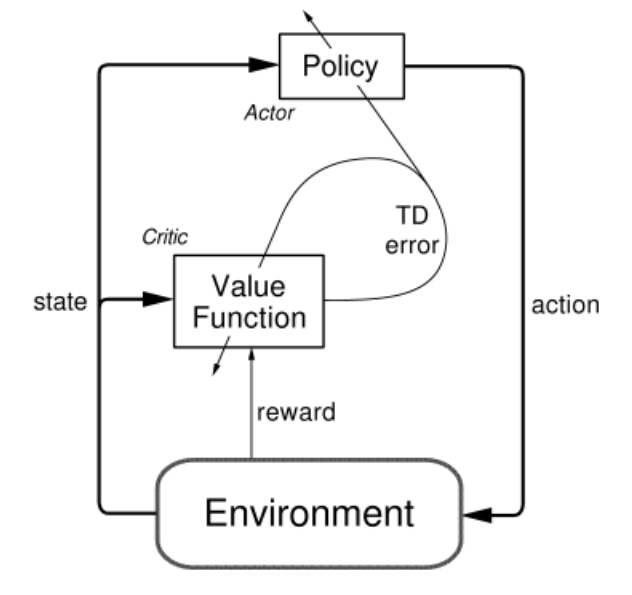
\includegraphics[height=0.5\textwidth]{img/actorcritic.png}
	\caption{\small Actor-critic architecture schema: the actor represents the policy and maps the input state to an output action, while the critic represents the value function. Both networks can be updated with, e.g.  the TD-error, using the contribution of the critic. It is noticeable that the actor uses the critic during the learning process \cite{sutton2018reinforcement}.}
	\label{fig:actorcritic}
\end{figure}

\subsection{Deep Deterministic Policy Gradient (DDPG)} \label{ddpg}

Deep Deterministic Policy Gradient (DDPG) \cite{lillicrap2015continuous} is a policy gradient algorithm that works learning a Q-function and a policy, and that grows from the deterministic policy gradient algorithm (DPG) \cite{silver2014deterministic}. It is a model-free, off-policy, actor-critic algorithm which utilises deep function approximators to learn policies in high-dimensional, continuous action spaces. It can be applied to situations that can not be solved using \textit{DQN} algorithm \cite{mnih2015human} because of the presence of continuous action spaces. A fine discretisation of the action space to adapt the situation to DQN would lead to an explosion in the number of discrete actions and the curse of dimensionality.
\textit{Bellman equation} and \textit{Q-learning} are integral parts of this algorithm. The algorithm concurrently learns a Q-value function and a policy: it uses off-policy data and the Bellman equation to learn the Q-value function and uses the Q-value function to learn the policy.

Usually, in Reinforcement Learning, if the optimal action-value function $Q^*(s,a)$ is known, then in any given state, the optimal action $a^*(s)$ can be found by solving \vref{eq:besta}.
\begin{equation} \label{eq:besta}
	a^*(s) = \arg \max_a Q^*(s,a)
\end{equation}
When the number of discrete actions is finite, calculating the $\max$ poses no problem, because the Q-values can be calculated for each action separately, then directly compared. However, when the action space is continuous, this process becomes highly non-trivial: it would need to be run at every step of the episode, whenever the agent wants to take any action in the environment, and this can not work.

Because the action space is continuous, the function $Q^*(s,a)$ is presumed to be differentiable concerning the action argument. For this reason, an efficient, gradient-based learning rule for a policy $\pi(s)$ which exploits that fact can be set up, approximating it with $\max_a Q(s,a) \approx Q(s,\pi(s))$.

\subsubsection{Target Networks} \label{targetnet}

DDPG algorithm exploits 4 neural networks: the \textit{local actor}, the \textit{local critic}, the \textit{target actor} and the \textit{target critic}. Actor networks aim is to approximate the policy using parameters $\theta$ while critic networks approximate the Q-Value function using parameters $\phi$.

Initially, actor and critic networks have both randomly initialised parameters. Then the local actor -- the current policy -- starts to propose actions to the agent, given the current state, starting to populate the experience replay buffer.

When the replay buffer is big enough, the algorithm starts to sample randomly a mini-batch of experiences for each timestep $t$. This mini-batch is used to update the local critic minimising the Mean Squared Error (MSE) between the local Q-value and the target one shown in \vref{eq:ddpgmse} where $y_i = y_t$ given by \vref{eq:ddpgloss} and to update the actor policy using the sampled policy gradient defined in \vref{eq:mean_gradient}.
\begin{equation}\label{eq:ddpgmse}
	L = \frac{1}{N} \sum_i(y_i -Q(s_i, a_i|\phi))^2
\end{equation}
We can imagine the target networks as the \textit{labels} of supervised learning.

Also the target networks are updated in this \textit{learning step}. A mere copy of the local weights is not an efficient solution, because it is prone to divergence. For this reason, a \textit{soft} target updates is used. It is given by \vref{eq:softupdate} where $\tau \ll 1$.
\begin{equation} \label{eq:softupdate}
	\theta' \leftarrow \tau \theta + (1-\tau)\theta
\end{equation}


\subsubsection{Learning Equations}

The two fundamental functions in Reinforcement Learning exploited in DDPG are the \textit{action-value function} -- see \vref{eq:actionvalue} -- and the correspondent \textit{Bellman equation} -- see \vref{eq:bellman}.
If this policy is deterministic we can describe it as a function $ \pi : \mathcal{S} \leftarrow \mathcal{A}$ obtaining \vref{eq:bellman2} which depends only on the environment.
\begin{equation}\label{eq:bellman2}
	Q^\pi(s_t, a_t) = \mathbb{E}_{r_t,s_{t+1}\sim \mathit{E}}[r(s_t, a_t) + \gamma Q^\pi(s_{t+1}, \pi(s_{t+1}))]
\end{equation}
This means that it is possible to learn $Q^\pi$ off-policy, using transition generated by a different stochastic behaviour policy $\beta$.

Focusing more and more on DDPG, the Bellman equation is the starting point for learning an approximator to $Q^*(s,a)$ of Q-Learning. The approximator is parametrised by $\phi$ and the value network is updated and optimised by minimising the loss defined in \vref{eq:ddpgloss} where $d_t$ is a flag which indicates whether the  state $s_{t+1}$ is terminal.
\begin{equation}\label{eq:ddpgloss}
	\begin{gathered}
		L(\phi) = \mathbb{E}_{s_t\sim \rho^\beta, a_t\sim \beta,r_t\sim E}[(Q(s_t, a_t|\phi)-y_t)^2] \\
		y_t = r(s_t, a_t) + \gamma (1-d_t)Q(s_{t+1}, \pi(s_t+1)|\phi)
	\end{gathered}
\end{equation}
It is clear from the \vref{eq:ddpgloss} that the loss is calculated starting from the transitions generated by the policy $\beta$. For this reason a great importance in this algorithm is given to \textit{replay buffer} -- see \vref{experience} -- and \textit{target networks} -- see \vref{targetnet}.

From the policy perspective, the objective is to maximise \vref{eq:expected} calculating the policy loss through the derivative of the objective function with respect to the policy parameter \vref{eq:derivative_exp}. However, since the algorithm is updating the policy in an off-policy way with batches of experience, it is possible to use the mean of the sum of gradients calculated from the mini-batch \vref{eq:mean_gradient}.

\begin{equation}\label{eq:expected}
	J(\theta) = \mathbb{E}[Q(s,a)|_{s=s_t,a=\pi(s_t)}]
\end{equation}
\begin{equation}\label{eq:derivative_exp}
	\nabla_{\theta} J(\theta) \approx \nabla_a Q(s,a) \nabla_{\theta}\pi(s|\theta)
\end{equation}
\begin{equation}\label{eq:mean_gradient}
	\nabla_{\theta} J(\theta) \approx \frac{1}{N}\sum_{i}\big[\nabla_a Q(s,a| \phi)|_{s=s_i, a = \pi(s_i)} \nabla_{\theta}\pi(s|\theta)|_{s=s_i}\big]
\end{equation}
\Vref{ddpgalg} shows the pseudocode of the DDPG algorithm.

\subsubsection{Exploration vs. Exploitation}
In reinforcement learning for discrete action spaces, exploration is done selecting a random action (e.g.\ epsilon-greedy). For continuous action spaces, exploration is done adding noise to the action itself. In \cite{lillicrap2015continuous}, the authors use Ornstein-Uhlenbeck process \cite{uhlenbeck1930theory} to add noise to the action output $
	a_t = \pi(s_t|\theta) + \mathcal{N}$. After that the action is clipped in the correct range.

\subsubsection{Hyperparameters} \label{hpddpg}

\paragraph{Exploration noise} The exploration noise consists of two sets of parameters. The first set refers to the Ornstein-Uhlenbeck Process noise parameters $\pi, \sigma, \theta$ as reported in \cite{uhlenbeck1930theory}. The second one consists of the parameters of $\epsilon$, a small value to decrease the impact of the noise on the action. \Vref{eq:epsilon} describes how the impact of the noise decreases in function of the current episode number $e$, where $\epsilon_{\text{start}}$ represent the starting value of the noise and $\epsilon_{\text{end}}$ the final one.

\begin{equation} \label{eq:epsilon}
	\epsilon = \epsilon_{\text{start}} - (\epsilon_{\text{start}} -\epsilon_{\text{end}}) \min\Bigg(1.0, \frac{e}{\epsilon_{\text{decay}}}\Bigg)
\end{equation}

\paragraph{Replay buffer} The parameters available for replay memory are its maximum size, its minimum size to start the learning phase and the mini-batch size to sample for each learning step.

\paragraph{Neural Network} The neural network can be considered as a whole complex hyperparameter because it is possible to select among different layers to exploit for specific problems -- e.g. \ the number of layers, the type of layers, the number of hidden features. Given the network architecture, the primary neural networks hyperparameters are the learning rate $\alpha$ and the update method -- e.g.\ Adaptive Momentum Estimation (ADAM).

\paragraph{Learning Update} The parameters of the learning phase of the algorithm are mainly two. The first one is $\gamma$, the main parameter in the reinforcement learning framework, which characterises the discounted return. The second is the soft target update parameter $\tau$, which determinates the entity of the update of the network at each learning step.

\begin{algorithm}[!h]
	\SetAlgoLined
	\small
	\DontPrintSemicolon
	\LinesNumbered
	\KwIn{Initial critic network parameter $\phi$ and actor network parameter $\theta$}

	Initialise target network weights $\bar{\phi} \leftarrow \phi$, $\bar{\theta} \leftarrow \theta$\;
	Initialise a random process $\mathcal{N}$ for action exploration\;
	\For{episode = 1, M}{
		Receive the initial observation state $s_t \leftarrow s_1$\;
		\Repeat{$s_t$ is terminal}{
			Select action $a_t = \pi(s_t|\theta) + \mathcal{N}$ and \textit{clip} results\;
			Execute action $a_t$ and obtain tuple $(r_t, s_{t+1}, d_t)$\;
			Store transition $(s_t, a_t, r_t, s_{t+1}, d_t)$ in $\mathcal{D}$\;
			\If{it is time to update}{
				Sample random minibatch of $N$ transitions $(s_t, a_t, r_t, s_{t+1}, d_t)$ from $\mathcal{D}$\;
				Compute the target $y_i = r_i + \gamma (1-d_i) Q'(s_{i+1}, \pi'(s_{i+1}|\theta)|\phi)$\;
				$\phi \leftarrow \phi - \lambda_Q \nabla_{\phi}J_Q(\phi)$ \tcp*{Update critic}
				$\theta \leftarrow \theta - \lambda_\pi \nabla_\theta J_\pi(\theta)$\tcp*{Update actor}
				$\phi \leftarrow \tau \phi +(1-\tau)\phi$ \tcp*{Soft update critic}
				$\theta \leftarrow \tau \theta +(1-\tau)\theta$\tcp*{Soft update critic}
			}
			$s_t \leftarrow s_{t+1}$
		}

	}
	\KwOut{Optimised parameters $\theta$ and $\phi$\;}
	\caption{DDPG Algorithm \cite{lillicrap2015continuous}}
	\label{ddpgalg}
\end{algorithm}
%\begin{figure}[!h]
%	\begin{center}
%		\begin{tikzpicture}
%		[node distance=1.5cm]
%		\node[object] (state)  {State $s_t$};
%		\node[element, below of=state] (linear1){\texttt{ReLu(Linear(in=$S$, out=256))}
%		};
%		\node[element, below of=linear1] (linear2){\texttt{ReLu(Linear(in=256, out=256))}
%		};
%		\node[element, below of=linear2] (linear3){\texttt{Tanh(Linear(in=256, out=$A$))}
%		};
%		\node[object, below of=linear3] (action){ Action $a_t$};
%		
%		\draw[arrow] (state) -- (linear1);
%		\draw[arrow] (linear1) -- (linear2);
%		\draw[arrow] (linear2) -- (linear3);
%		\draw[arrow] (linear3) -- (action);
%		\end{tikzpicture}
%		\begin{tikzpicture}
%		[node distance=1.5cm]
%		\node[object, left of=action] (state)  {State $s_t$ };
%		\node[object, right of=state] (action)  {Action $a_t$};
%		\node[element, below= of $(state)!0.5!(action)$] (linear1){\texttt{ReLu(Linear(in=$S+A$, out=256))}
%		};
%		\node[element, below of=linear1] (linear2){\texttt{ReLu(Linear(in=256, out=256))}
%		};
%		\node[element, below of=linear2] (linear3){\texttt{Linear(in=256, out=1)}
%		};
%		\node[object, below of=linear3] (value){ Q-value $q_t$};
%		
%		\draw[arrow] (state) -- (linear1);
%		\draw[arrow] (action) -- (linear1);
%		\draw[arrow] (linear1) -- (linear2);
%		\draw[arrow] (linear2) -- (linear3);
%		\draw[arrow] (linear3) -- (value);
%		%\draw [draw, -latex',thick] (3.east) -- ++(2,0) node(lowerright){} |- (state.east);
%		
%		\end{tikzpicture}
%	\end{center}		
%	\caption{Actor and Critic Networks: $S$ is the length of the array of states, while $A$ is the length of the array of actions.}
%	\label{fig:actor_critic_schema}
%\end{figure}

\subsection{Soft Actor-Critic (SAC)} \label{sac}

Soft Actor-Critic (SAC) \cite{haarnoja2018soft, haarnoja2018alg} combines the off-policy actor-critic setup with a stochastic policy (actor), devising a bridge between stochastic policy optimization and DDPG-style approaches.
As DDPG, SAC can work in situations characterised by the presence of continuous action spaces, and it is a model-free, off-policy and actor-critic algorithm.

SAC algorithm can overcome some of the problems of DDPG.
The latter can achieve excellent performance, but the interaction between the deterministic actor-network and the Q-function makes it difficult to stabilise and brittle concerning hyperparameters and other kinds of tuning \cite{duan2016benchmarking,henderson2018deep}. The learned Q-function begins to dramatically overestimate Q-values, which then leads to the policy breaking because it exploits the errors in the Q-function. For this reason, SAC exploits \textit{Clipped Double-Q Learning} also used by Twin Delayed DDPG (TD3) \cite{fujimoto2018addressing}. It learns two Q-functions instead of one and uses the smaller of the two Q-values to form the targets in the Bellman error loss functions.

Another feature of SAC is \textit{entropy regularization} \cite{ziebart2008maximum, toussaint2009robot, rawlik2013stochastic, fox2015taming, haarnoja2017reinforcement}. The policy is trained to maximise a trade-off between expected return and entropy, a measure of randomness in the policy. This peculiarity is strongly related to the exploration-exploitation trade-off: increasing entropy results in more exploration, which can accelerate learning later on, but it can also prevent the policy from prematurely converging to a local optimum.


\subsubsection{Target Networks}
SAC algorithm exploits 5 neural networks: the local stochastic policy network with parameter $\theta$, two local Q-Networks with parameters  $\phi_1$, $\phi_2$ respectively, two target Q-Networks with parameters $\bar{\phi_1}$ and $\bar{\phi_2}$ respectively.
Their behaviour is the same as the one of DDPG target network: the algorithm updates the target networks following \vref{eq:softupdate}.

\Vref{sacalg} shows the pseudocode of the SAC algorithm.

\subsubsection{Entropy-Regularised Reinforcement Learning}

\textit{Entropy} represents the average rate at which a stochastic source of data produces information. It is, in simple terms, a quantity which describes how random a random variable is.
The motivation behind the use of entropy is that when the data source produces a low-probability value, the event carries more information than when the source data produces a high-probability value.

Let $x$ be a random variable with probability mass or density function $P$. The entropy $\mathcal{H}$ of $x$ is computed from its distribution $P$ according to \vref{eq:entropy}.
\begin{equation} \label{eq:entropy}
	\mathcal{H}(P) = \mathbb{E}_{x \sim P} [- \log P(x)]
\end{equation}
In \textit{entropy-regularised} reinforcement learning the standard objective is generalised by augmenting it with entropy. The agent gets a bonus reward at each time step proportional to the entropy of the policy at that timestep. Assuming an infinite-horizon discounted setting, this changes the RL problem as shown in \vref{eq:entropy_return} where $\alpha > 0$ is the temperature parameter that determines the relative importance of the entropy term controlling the stochasticity of the optimal policy.
\begin{equation} \label{eq:entropy_return}
	\pi^* = \arg \max_{\pi} \mathbb{E}_{\tau \sim \pi}\Bigg[\sum_{t=0}^{\infty} \gamma^t \bigg(R(s_t, a_t, s_{t+1}) + \alpha \mathcal{H}(\pi(\cdot|s_t))\bigg)\Bigg]
\end{equation}
It is clear that the standard maximum expected return can be retrieved in the limit as $\alpha \rightarrow 0$.

From \vref{eq:entropy_return} it is possible to derive \textit{state-value function} $V^\pi(s)$ and \textit{action-value function} $Q^\pi(s,a)$ as shown in \vref{eq:state_value} and \vref{eq:action_value}.
\begin{equation} \label{eq:state_value}
	V^\pi(s) = \mathbb{E}_{\tau \sim \pi}\Bigg[\sum_{t=0}^{\infty} \gamma^t \bigg(R(s_t, a_t, s_{t+1}) + \alpha \mathcal{H}(\pi(\cdot|s_t))\bigg)\bigg|s_0 = s\Bigg]
\end{equation}
\begin{equation} \label{eq:action_value}
	Q^\pi(s,a) = \mathbb{E}_{\tau \sim \pi}\Bigg[\sum_{t=0}^{\infty} \gamma^t R(s_t, a_t, s_{t+1}) + \alpha \sum_{t=1}^{\infty} \gamma^t \mathcal{H}(\pi(\cdot|s_t))\bigg|s_0 = s, a_0 =a\Bigg]
\end{equation}
From these equations is possible to derive the connection between state-value and action-value function given by \vref{eq:q_v_relation} and the Bellman equation given by \vref{eq:bellmanentropy}.
\begin{equation} \label{eq:q_v_relation}
	V^\pi(s) = \mathbb{E}_{a\sim\pi}[Q^\pi(s,a)] + \alpha \mathcal{H}(\pi(\cdot|s))
\end{equation}
\begin{equation}
	\begin{aligned} 	\label{eq:bellmanentropy}
		Q^\pi(s,a) & = \mathbb{E}_{s'\sim P, a'\sim\pi}[R(s,a,s') + \gamma(Q^\pi(s',a') + \alpha \mathcal{H}(\pi(\cdot|s')))] \\
		           & = \mathbb{E}_{s'\sim P}[R(s,a,s') + \gamma V^\pi(s')]
	\end{aligned}
\end{equation}

\subsubsection{Learning Equations}
SAC algorithm learns a policy $\pi_\theta$ with $\theta$ parameter set and two Q-functions $Q_{\phi_1}$,  $Q_{\phi_2}$ with $\phi_1$ and $\phi_2$ parameter sets respectively.
The state-value function is implicitly parametrised through the soft Q-function parameters thanks to \vref{eq:vsac}.
In \cite{haarnoja2018soft} a function approximator for this function was introduced, but later \cite{haarnoja2018alg} the authors found it to be unnecessary.
\begin{equation} \label{eq:vsac}
	\begin{aligned}
		V^{\pi}(s) & = \mathbb{E}_{a \sim \pi}[Q^{\pi}(s,a)] + \alpha \mathcal{H} \left(\pi(\cdot|s)\right)               \\
		           & = \mathbb{E}_{a \sim \pi}[Q^{\pi}(s,a) - \alpha \log \pi(a|s)]                                       \\
		           & \approx Q^{\pi}(s,\tilde{a}) - \alpha \log \pi(\tilde{a}|s), \;\;\;\;\; \tilde{a} \sim \pi(\cdot|s).
	\end{aligned}
\end{equation}

\paragraph{Learning Q} Q-functions are learned by Mean Squared Bellman Error (MSBE) minimization, using a target value network to form the Bellman backups using \vref{eq:lossQ}. \Vref{eq:vsac} implicitly parametrise the state-value function.

\begin{equation} \label{eq:lossQ}
	J_Q(\phi_i) = \mathbb{E}_{(s_t,a_t) \sim \mathcal D}\left[ \frac{1}{2}\Bigg( Q_{\phi_i}(s_t,a_t) - \left(r(s_t, a_t) + \gamma \mathbb{E}_{s_{t+1} \sim p} V_{\bar{\phi_i}}(s_{t+1}) \right) \Bigg)^2 \right]
\end{equation}


The update shown makes use of target soft Q-function with parameters $\phi_i$, which are calculated, like in the DDPG algorithm, as an exponentially moving average of the soft Q-function parameters \cite{mnih2015human}. It can be optimised using stochastic gradients.

\paragraph{Learning the Policy} It is possible to derive SAC starting from the definition of soft policy iteration demontrated in   \cite[Section 4]{haarnoja2018alg}. In particular, the policy has to be learned starting from the minimization of the expected KL-divergence \cite{kullback1959information,kullback1951information} and exploiting \vref{eq:policysac}.
\begin{equation} \label{eq:policysac}
	J_\pi(\theta) = \mathbb{E}_{s_t \sim \mathcal{D}}[\mathbb{E}_{a_t \sim \pi_\theta}[\alpha \log \pi_\theta(a_t|s_t) - Q_\phi(s_t,a_t)]]
\end{equation}
As \cite{haarnoja2018alg} reports, there are several options for the minimization of $J_\pi(\theta)$, but the most straightforward one using neural network as function approximator is to apply the \textit{reparametrization trick}.
It works reparametrising the policy using a neural network transformation following \vref{eq:reparametrise} where $\epsilon_t$ in a noise vector sampled from some fixed distribution.
\begin{equation} \label{eq:reparametrise}
	a_t = f_\theta(\epsilon_t; s_t)
\end{equation}
Therefore, it is possible to rewrite the expectation over actions in \vref{eq:policysac} into an expectation over noise as in \vref{eq:policysac1}.
\begin{equation} \label{eq:policysac1}
	J_\pi(\theta) = \mathbb{E}_{s_t \sim \mathcal{D}, \epsilon_t \sim \mathcal{N}}[\alpha \log \pi_\theta(f_\theta(\epsilon_t; s_t)|s_t) - Q_\phi(s_t,f_\theta(\epsilon_t; s_t))]
\end{equation}
To get the policy loss, the final step is to substitute $Q_{\phi}$ with one of our function approximators: the choice falls $\min_{i=1,2}Q_{\phi_i}(s_t, f_\theta(\epsilon_t; s_t))$, as suggested from the authors of \cite{haarnoja2018alg}.

\subsubsection{Exploration vs. Exploitation} \label{alphasac}
SAC algorithm trains a stochastic policy using \textit{entropy regularization}. $\alpha$ is the entropy regularisation coefficient which is the parameter that explicitly controls the exploration-exploitation trade-off. A higher $\alpha$ corresponds to more exploration, while a lower $\alpha$ corresponds to more exploitation.

This parameter has fundamental importance in the algorithm, and it may vary from environment to environment. Choosing the optimal $\alpha$ parameter is a non-trivial task that could require careful tuning in order to find the one which leads to the stablest and highest-reward learning. In \cite[Section 5]{haarnoja2018alg}, the authors formulated a different maximum entropy reinforcement learning algorithm to overcome this problem.
Forcing the entropy to a fixed value is a weak solution because the policy should be free to explore more where the optimal action is uncertain, and to exploit the learned mapping in states with a more clear optimal action.
The gradients are computed using \vref{eq:alphalearn}
\begin{equation} \label{eq:alphalearn}
	J(\alpha) = \mathbb{E}_{a_t \sim \pi}[-\alpha \log\pi(a_t|s_t) - \alpha \bar{\mathcal{H}}]
\end{equation}
During the test phase, the algorithm uses the mean action instead of a  sample from the distribution learned. This choice tends to improve performance over the original stochastic policy, allowing to see how well the policy exploits what it has learned.

\subsubsection{Hyperparameters}

\paragraph{Entropy regularisation parameter} The only parameter of this section is $\alpha$. It can be set as constant through all the training or it can be learned thanks to the approach described in \cite{haarnoja2018alg}. Further details in \vref{alphasac}.
\paragraph{Replay buffer} See \vref{hpddpg}.
\paragraph{Neural Network} See \vref{hpddpg}.
\paragraph{Learning Update} See \vref{hpddpg}.

\begin{algorithm}[!h]
	\SetAlgoLined
	\small
	\DontPrintSemicolon
	\LinesNumbered
	\KwIn{Initial policy parameter $\theta$ and Q-function parameters $\phi_1,\phi_2$\;}
	Initialise target network weights $\bar{\phi_1 }\leftarrow \phi_1,\bar{\phi_2 } \leftarrow \phi_2$\;
	Initialise an empty replay buffer $\mathcal{D}$\;
	\For{episode = 1, M}{
	Receive initial state $s_t \leftarrow s_1$\;
	\Repeat{$s_t$ is terminal}{
	Observe state $s_t$ and select action $a_t \sim \pi_\theta(\cdot|s_t)$\;
	Execute $a_t$  and obtain tuple $(r_t, s_{t+1}, d_t)$\;
	Store $(s_t,a_t,r_t,s_{t+1},d_t)$ in replay buffer $\mathcal{D}$\;
	$s_t \leftarrow s_{t+1}$
	}
	}
	\If{it is time to update}{
		Sample random minibatch of $N$ transitions $(s_t, a_t, r_t, s_{t+1}, d_t)$ from $\mathcal{D}$\;
		Calculate targets\;
		$\phi_i \leftarrow \phi_i - \lambda_Q \nabla_{\phi_i}J_Q(\phi_i)$, for $i \in \{1, 2\}$\;
		$\theta \leftarrow \theta - \lambda_\pi \nabla_\theta J_\pi(\theta)$\;
		$\alpha \leftarrow \alpha - \lambda \nabla_\alpha J(\alpha)$\;
		$\bar{\phi_i} \leftarrow \tau \phi_i + (1-\tau) \bar{\phi_i}$, for $i \in \{1, 2\}$\\
	}
	\KwOut{Optimised policy parameter $\theta$ and Q-function parameters $\phi_1,\phi_2$\;}

	\caption{Soft Actor-Critic \cite{haarnoja2018alg}}
	\label{sacalg}
\end{algorithm}

\section{Related Work}

%\todomacaluso{
%	\begin{itemize}
%		\item Explanation of the state-of-the-art focusing more on Reda's paper, its approach and the related bibliography
%\item Increasing interest in Reinforcement Learning applied to real-world situations, in contrast with simulated environments experiments
%	\end{itemize}	
%}The project of this thesis aims to design a control system for a small toy robot called Anki Cozmo (see \vref{sec:cozmo}) and formalise the driving learning problem as a Markov decision process to enable the application of reinforcement learning algorithms.

A truly inspiring work for this thesis is \cite{kendall2019learning} where the authors show, probably for the first time, that deep reinforcement learning is a viable approach to autonomous driving. Nowadays,  most approaches focus on formal logic which determines driving behaviour using annotated 3D geometric maps: the external mapping infrastructure intuitively makes this approach limited to the models and the representation of the surroundings.
This technique is not able to scale up efficiently because of last-mentioned strong dependencies.

The fundamental concept underlying \cite{kendall2019learning} to make autonomous driving systems a ubiquitous technology is the design of a system which can drive relying - just like humans - on a comprehensive understanding of the immediate environment \cite{badrinarayanan2017segnet}.
\cite{ort2018autonomous} is useful to motivate the research in this direction because it represents an example of autonomous vehicle navigation exploiting GPS for coarse localisation and LIDAR to understand the local scene instead of detailed prior maps.
Many sensors have been developed through the years to gather information and observations increasingly sophisticated. However, the major problem is the massive budget needed to afford all these technologies.
The extraordinary results obtained by \cite{kendall2019learning} are not based on intelligent sensing techniques, but on the usage of a monocular camera image together with vehicle speed and steering angle.
They decided to apply the model-free approach of reinforcement learning because it is exceptionally general and useful to solve tasks that are complex to model correctly. As discussed previously in this chapter, model-based algorithms tend to be more data-efficient than model-free ones; however, the quality of the adopted model limits the results \cite{deisenroth2011pilco}.

The authors decided to exploit Deep Deterministic Policy Gradient (DDPG) \cite{lillicrap2015continuous}.
Firstly, they developed a 3D driving simulator using Unreal Engine 4 to tune reinforcement learning hyperparameters such as learning rates and number of gradient steps to take after each training episode. Then, they tried to apply the DDPG algorithm in the real world using the parameters learnt. They also did some experiments using a compressed state representation provided by a Variational Autoencoder \cite{kingma2013auto,rezende2014stochastic}.
The excellent results obtained in \cite{kendall2019learning} have been exceeded by the same authors in \cite{wayve2019human} that shows astonishing performances driving on narrow and crowded urban road never-seen during training.

Starting from all these outlined ideas, we decided to investigate ways and approach to autonomous driving with reinforcement learning without using simulators or prior data in order to make a step towards the so-called \textit{reinforcement learning in the wild} \cite{chara2018wild}. The most popular and prominent achievements in reinforcement learning to date consist of experiments done using simulated environments or ones which exploit the knowledge acquired in simulated environments in real ones.
The team of the DeepMind manages to develop smart agents capable of performing super-human results in numerous games and videogames such as \textit{Go} \cite{silver2016mastering,silver2017mastering}, while OpenAI engineers an agent capable of beating the world champion of the multi-player Dota 2 game \cite{openai2018dota,openai2019dota}.  These problems are not easy to solve but have the benefit of having a training environment equal to the test one. This fact does not apply to the approach which exploits simulated experiments results in real environments.

The last-mentioned method encloses a critical caveat: the awareness that the simulator has limits.
Unlike what happens in some environments where there are many similarities between the simulator and the environment -- e.g.\ games and videogames --, in harder environments -- e.g.\ autonomous vehicle on public roads, ads marketplaces, biology, and applications around human behaviour -- is very difficult to get a simulator capable of reproducing with  high-fidelity the wild environment because of approximations that could mislead the learning.
On the other hand, learning directly on the environment need a fast learning cycle because of the significant number of interaction with the environment and, above all, cheap or low-risk exploration cost: millions of self-driving episodes in simulator ending with a crash of the car has a small cost in respect of one episode with the same ending crash in the real world.

Between the end of 2018 and the beginning of 2019, UC Berkeley and Google developed jointly a state-of-the-art off-policy model-free reinforcement learning algorithm called soft actor-critic (SAC) (see \vref{sac}). The critical goal is to provide a deep RL algorithm suitable for real-world problems and the related new challenges that they pose.
They outlined the desired properties of the ideal deep reinforcement learning algorithm:
\begin{description}
	\item[Sample Efficiency:] the process of learning in the real world can be a very time-consuming task. For this reason, it is desirable a functional sample complexity to learn skills successfully.
	\item[No sensitive hyperparameters:] as mentioned before, hyperparameter tuning could be a tough task to complete in real-world experiments as it could require numerous repetitions in situations where the cost in terms of time and money could be burdensome. The proposed solution of the authors is maximum entropy RL which provides a robust framework that minimises the need for hyperparameter tuning.
	\item[Off-policy learning:] this learning approach allows the reuse of collected data for various tasks. This possibility helps the process of prototyping a new task when adjusting parameters or choosing a different reward function.
\end{description}

Soft actor-critic (SAC) represents a deep RL algorithm capable of satisfying the previously mentioned requirements. The authors of \cite{haarnoja2018soft,haarnoja2018alg} revealed that the algorithm is capable of solving real-world robotic tasks in a conspicuous but acceptable number of hours, showing its robustness to hyperparameters and working on a large variety of simulated environments always using the same set of parameters.
Not only it shows great performances in numerous challenging tasks compared to deep deterministic policy gradient (DDPG), twin delayed deep deterministic policy gradient (TD3) \cite{fujimoto2018addressing} and proximal policy optimisation (PPO) \cite{schulman2017proximal}, but reveals its power by solving three tasks from scratch without relying on simulators or demonstrations \cite{bair2019soft}.

The real-world robotic task involving a 3-finger dexterous robotic hand to manipulate an object similar to a sink faucet with a coloured end presented in \cite[Section 7.3]{haarnoja2018alg} shows similar concepts to the task analysed in this thesis for what concerns the framework of deep reinforcement learning exploited. The algorithm exploits raw RGB images and processes them through a convolutional neural network. The final goal of the robot is to rotate the valve into the correct position -- with the coloured part pointing to the right -- starting from a random position for each episode. The results obtained represents one of the most sophisticated real-world robotic manipulation tasks learned end-to-end with deep reinforcement learning, starting from raw images and without any previous simulation or pretraining phase.

Taking all arguments into account, we decided to follow \cite{kendall2019learning} implementing a similar self-driving framework based on the design of a control system for a small toy robot called Anki Cozmo (see \vref{ch4}). Therefore, we formalise the autonomous driving learning problem as a Markov decision process to enable the application of reinforcement learning algorithms, taking into account the improvements mentioned in this section about model-free reinforcement learning algorithms applied to real-world robotic problems. \Vref{ch4} provides a detailed description of the choice made and the system design.








	%\todomacaluso{
%	\begin{itemize}
%		\item General description of the framework
%		\item Discussion about the motivation and the importance of this framework, such as the necessity of a Reinforcement Learning Framework to test different algorithms with different environments providing the same interface.
%		\item One contribution of the thesis: the creation and design of an OpenAI Gym environment for Anki Cozmo Environment with connection to chapter 4.
%	\end{itemize}	
%}

\chapter{Tools and Frameworks}

This chapter aims to describe the main tools and frameworks used to develop the project of this thesis. The first section will describe OpenAI Gym framework, a central toolkit for developing and comparing reinforcement learning algorithms, and explain why this tool is essential for reinforcement learning research.
The second part of this chapter will outline Cozmo, the powerful toy robot developed by Anki that we used as an agent in the reinforcement learning scenario to apply algorithms to try solving autonomous self-driving tasks: \vref{ch5} will report the analysis and description of these experiments. This section will also report a set of available alternatives to Cozmo, explaining the motivations underlying the final choice.
The description about PyTorch, an optimised tensor library for deep learning using GPUs and CPUs used to build up the convolutional neural network of this work, and the related comparison with TensorFlow will occupy the last part of this chapter.

\section{OpenAI Gym}

Nowadays, OpenAI Gym, released in 2016 with its public beta, is one of the most popular toolkits and frameworks in the reinforcement learning scenario. A brief analysis of reinforcement learning research could be useful to outline the motivations underlying the need for a reinforcement learning framework.

As reported previously in  \vref{ch2} reinforcement learning is a subfield of machine learning dedicated to the world of decision making and motor control: researchers study how an agent can learn and improve to achieve a specific goal in a complex, usually unknown environment. This machine learning paradigm is becoming more and more attractive for both researchers and industries because of its visionary property of being very general. A reinforcement learning algorithm can be exploited to control a robot's motor in order to make it capable of running or jumping, play a videogame or a board game, make critical business decisions like pricing and inventory management, but also learn how to invest in financial trading environments. The generality of reinforcement learning became engaging thanks to the remarkable results achieved in many challenging environments, as reported previously in \vref{ch2}.

Despite these appealing features, the research was slowed down by other circumstances, no less critical.
The need for better benchmarks represents the first factor. As an example, the abundant availability of conspicuous datasets like \textit{ImageNet} \cite{deng2009imagenet} has driven supervised learning improvement in the research. For what concerns reinforcement learning, the nearest equivalent to supervised learning datasets would be a broad collection of different environments in order to test various algorithms with different kinds of observations or rewards.
The second withdraw of this approach to learning is the lack of standardisation of environments designed in publications. In reinforcement learning, subtle differences in problem definition, reward function design or action space typology could make the difficulty of the task grow.  This fact threatens to slow down and corrupts experiments reproducibility making an objective comparison between the results of different papers almost impossible.

The need to fix both problems was the primary motivation behind the design and implementation of OpenAI Gym.

\subsection{Environments}

The agent and the environment represent the main components of reinforcement learning. The choice of OpenAI was to implement and provide the abstraction mainly for environments, not for agents. They decide to provide a standard environment interface instead of forcing the developer to use pre-defined agent interfaces: the motivation behind this choice was to leave developers independent in the design of the agent, the core of reinforcement learning, and facilitate the creation and usage of environments. Thanks to this approach, all agents implemented with OpenAI Gym can be used with the whole set of environments provided by the framework. Therefore, it is possible to create a personalised environment to suit the needs of a specific experiment that can be used by all agents exploiting OpenAI Gym environment interfaces.

In this scenario, we realised the first contribution to our thesis. Thanks to this framework features, we implemented an OpenAI Gym environment capable of interacting with Anki Cozmo by providing a binding between functions of Cozmo SDK and interfaces of the reinforcement learning framework. In \vref{ch4} we will provide further information and details about our contribution.

The importance related to the high quantity of environment is fundamental to build a reliable and sustainable framework for reinforcement learning algorithms. For this reason, OpenAI Gym contains a various and heterogeneous environment database, ready to be used.

\subsubsection{Interface Functions}

EExploring OpenAI Gym, it is essential to focus on the most crucial interface functions that the agent will exploit to interact with the environment.
The functions which constitute the skeleton of an OpenAI Gym environment are the following:
\begin{itemize}
    \item \texttt{def step(self, action)}: through this function, the agent can communicate the action it wants to take. The input data depends on the type and number of variables in the actions space (e.g.\ discrete or continuous). As will be discussed in \vref{ch3:observations}, the values returned by this function represent the environment state after the manipulation caused by the agent action. Thanks to these data, the agent will be able to select the next action following the reinforcement learning loop.
    \item \texttt{def reset(self)}: during the episode, internal variables of the environment changes, influenced by the action taken previously. This function allows the agent to restart the initial situation of the environment. This procedure is particularly helpful when an episode finishes and the agent has to restart the next learning episode in a brand new copy of the environment.
    \item \texttt{def render(self, mode='human', close=False)}: this function is mainly used in simulated environments. It enables the visual render (if available) of the environment.
 \item \texttt{def close(self)}: the final function to close the environment after the end of all experiments and episodes.
\end{itemize}

\subsubsection{Available environments}

To date, OpenAI Gym includes the following environments:
\begin{itemize}
    \item \textbf{Algorithms}: learning to imitate computations, such as copying or reversing symbols from the input tape, is the main aim of this typology. These environments might seem easy to be solved by a computer, but it is important to remember that the objective here is to learn to solve these tasks purely from examples. Therefore, it is possible to vary the sequence length to increase or decrease task difficulties easily. 
    \item \textbf{Atari}: \textit{Atari 2600} is a home video game console developed in 1977 which spread the use of general-purpose CPUs into gaming with game code distributed through cartridges. This environment section provides a database which contains more than 100 environments emulating Atari 2600 videogames. OpenAI Gym exploits \textit{Arcade Learning Environment (ALE)} \cite{bellemare2013arcade} providing RAW pixel images or RAM as observation of the environment.
	\item \textbf{Box2D}: in this group is possible to find some continuous control tasks in a simple 2D simulator such as \textit{BipedalWalker}, \textit{CarRacing} and \textit{LunarLander}
	\item \textbf{Classic Control}: this class provides a set of problem borrowed by control theory and widely exploited in the classic reinforcement learning literature. Some task examples are balancing a pole on a cart or swing up a pendulum.
	\item \textbf{MuJoCo}: this collection contains continuous control tasks running in a fast physics three-dimensional simulator called \textit{MuJoCo} which stands for \textit{Multi-Joint dynamics with Contact}. This physics engine aims to facilitate research and development in robotics, biomechanics, graphics and animation. The simulator is particularly suitable for model-based optimisation allowing to scale up computationally-intensive techniques.
Thanks to its features, it became useful as a source for reinforcement learning algorithms. \cite{todorov2012mujoco}
	\item \textbf{Robotics}: OpenAI released this algorithm typology to provide eight robotics environments with manipulation tasks significantly more difficult than the MoJoCo ones. It contains \textit{Fetch}, a robotic arm to move and grab objects, and \textit{ShadowHand}, a robotic hand to manipulate and grab pens, cubes and balls. \cite{ingredientsRoboticsResearch}
\end{itemize}

\subsection{Observations} \label{ch3:observations}

As previously reported, the \texttt{step(self, action)} environment interface is the most important one because it contains the behaviour definition of the environment that reacts to agent actions. 
Indeed, the agent has to know in which way its actions are influencing the environment in order to stop doing random actions and start making valuable decisions.

In order to provide this type of information to the agents, the \texttt{step} function returns four relevant values that reinforcement learning algorithms can exploit to determine the best action to do in the future. 
These values are:
\begin{itemize}
    \item \textbf{\texttt{observation (object)}}: a specific object which represents the environment observation and shows the changes provoked by agent actions. Its structure and interpretation depend on the implementation of the specific environment. For example, it could represent the raw pixel data from a camera, the status of a board game or physics data of a robot (joint angles and velocities).
    \item \textbf{\texttt{reward (float)}}: this is the fuel of the reinforcement learning algorithms. This value represents the reward achieved thanks to the action taken by the agent. The reward for each action can change among environments, but this is the crucial information to enable the agent to learn.
    \item \textbf{\texttt{done (boolean)}}: this value is a simple boolean that signals the agent when the episode ended and it is time to reset the environment to start a brand new episode. 
    \item \textbf{\texttt{info (dict)}}: a Python dictionary to monitor and show diagnostic information useful for debugging. The agent could use it as additional information in the learning process, but the documentation of OpenAI Gym does not recommend to use this data in the learning process to maintain the coherence with the reinforcement learning loop. 
\end{itemize}

The last important thing to report about OpenAI Gym framework is the definition of \texttt{Spaces}. As reported in the second chapter, an environment consists of the action space and the observation space. Both can provide discrete or continuous values: this distinction is fundamental to determine the usage of a specific algorithm rather than others to solve a given task better. For this reason, OpenAI Gym provides \texttt{Discrete} and \texttt{Box} to initialise discrete and continuous spaces, respectively. It allows the user to define a lot of features useful in the learning process, such as a maximum and minimum value setup or a default function to instantly sample a random value from the defined space.

\section{Anki Cozmo}

Especially in the latest decades, human beings have started a complicated relationship with robots. They are very fascinated by the prospect of artificial intelligence offered by recent researches and applications. However, they are apprehensive and worried at the same time because of the apocalyptic plot that many sci-fi films show and the big promise of automation, capable of replacing human workers in the future.
However, all these concerns disappear after meeting Cozmo, the palm-sized toy robot developed by the San Francisco-based company Anki and available on the market since 2016.
On first glance, Cozmo might appear as one of the cutest toy robots: not surprisingly Anki employed the guidance of Carlos Baena, the former Pixar animator, to design this robot.
Therefore, it can interact with people using a small display screen together with audio effects to mimic human emotional reactions and responses.
The result is a toy robot WALL-E-inspired both aesthetically and personality-wise, powered up by artificial intelligence to move and discover the surrounding environment. Thanks to the built-in camera, Cozmo can remember faces and recite names, but also to plan paths and play various games with its three cubes that carry sensors and lighting.

Despite these entertaining, but not so technical facts, Cozmo hides a lot of powerful features under the hood. Anki developers produced a high-quality Python SDK that allows developers to take control of the whole set of Cozmo sensors and actuators thanks to interaction granularity offered by functions and interfaces.
This section aims to outline the hardware and software architecture hidden underneath the cute Cozmo bodyworks, together with a comparison with the alternatives available to design the reinforcement learning system of this thesis. An essential inspiration in the writing of this section came from \cite{mellon2017cognitive}, \cite{touretzky2018cozmopedia} and Cozmo SDK Forums \footnote{Link: \href{https://forums.anki.com/}{https://forums.anki.com/}}.

\subsection{Cozmo Architecture}

It is possible to define Cozmo as a vision-guided mobile manipulator, one of the first consumer robot which can boast vision among its features. However, as reported before, the features it shows during the normal toy usage, do not equal the number of interfaces and functions made available to developers. The hardware and the software developed for Cozmo makes it the right choice to fast prototyping computer science projects: it is the main reason why we decided to exploit Anki Cozmo instead of other alternatives.
The SDK provided by Anki consists of a comprehensive set of low- and high-level functions which grants full access to sensor data providing the right flexibility, simplicity and granularity to satisfy every developer needs. It is versatile because it could be easily connected with hundreds of third-party libraries to augment Cozmo capabilities. Therefore, it is an entirely open-source SDK to give the community the freedom to customise and contribute.

\Vref{fig:cozmotear1,fig:cozmotear2} shows technologies, the hardware and software involved in the production of Cozmo. The first image represents stacks and connections between the robot core and the mobile application provided by Anki, while the second one shows the interaction between the last-mentioned application and the Python user program on the personal computer. The reader can retrieve a global perspective about the whole Cozmo architecture by merging these two figures.

\begin{figure}
	\tikzset{every picture/.style={line width=0.75pt}} %set default line width to 0.75pt        
	\scalebox{0.9}{
		\centering
		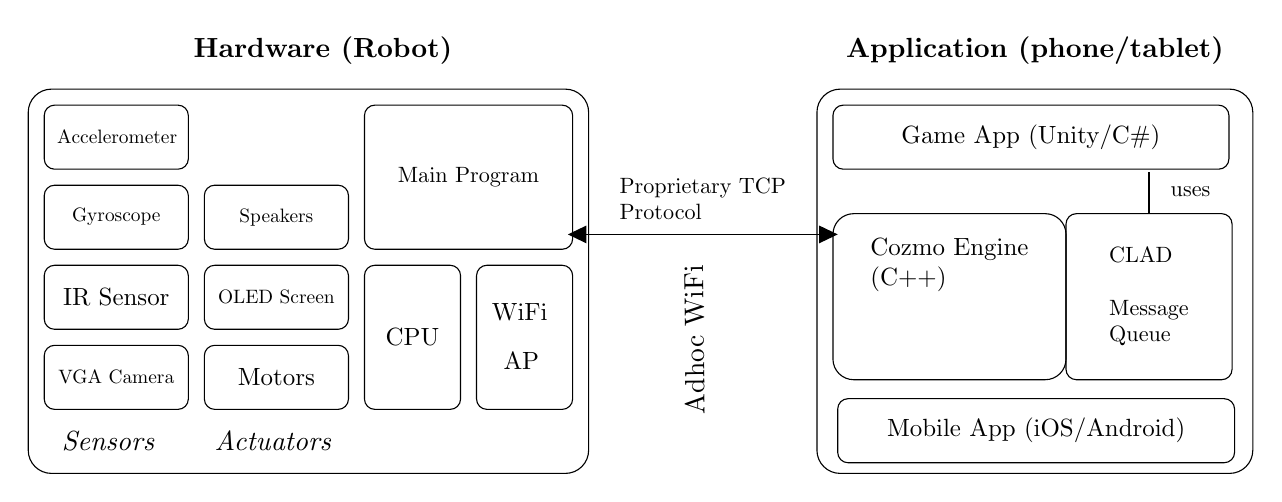
\begin{tikzpicture}[x=0.75pt,y=0.75pt,yscale=-1,xscale=1]
			%uncomment if require: \path (0,466); %set diagram left start at 0, and has height of 466

			%Shape: Rectangle [id:dp32857133822425977] 
			\draw  [fill={rgb, 255:red, 255; green, 255; blue, 255 }  ,fill opacity=1 ] (17.71,52.71) .. controls (17.71,49.95) and (19.95,47.71) .. (22.71,47.71) -- (82.14,47.71) .. controls (84.9,47.71) and (87.14,49.95) .. (87.14,52.71) -- (87.14,73.57) .. controls (87.14,76.33) and (84.9,78.57) .. (82.14,78.57) -- (22.71,78.57) .. controls (19.95,78.57) and (17.71,76.33) .. (17.71,73.57) -- cycle ;
			%Shape: Rectangle [id:dp46039429837534274] 
			\draw   (17.71,91.29) .. controls (17.71,88.52) and (19.95,86.29) .. (22.71,86.29) -- (82.14,86.29) .. controls (84.9,86.29) and (87.14,88.52) .. (87.14,91.29) -- (87.14,112.14) .. controls (87.14,114.9) and (84.9,117.14) .. (82.14,117.14) -- (22.71,117.14) .. controls (19.95,117.14) and (17.71,114.9) .. (17.71,112.14) -- cycle ;
			%Shape: Rectangle [id:dp38741871235010394] 
			\draw   (17.71,129.86) .. controls (17.71,127.1) and (19.95,124.86) .. (22.71,124.86) -- (82.14,124.86) .. controls (84.9,124.86) and (87.14,127.1) .. (87.14,129.86) -- (87.14,150.71) .. controls (87.14,153.48) and (84.9,155.71) .. (82.14,155.71) -- (22.71,155.71) .. controls (19.95,155.71) and (17.71,153.48) .. (17.71,150.71) -- cycle ;
			%Shape: Rectangle [id:dp004700439400786571] 
			\draw   (17.71,168.43) .. controls (17.71,165.67) and (19.95,163.43) .. (22.71,163.43) -- (82.14,163.43) .. controls (84.9,163.43) and (87.14,165.67) .. (87.14,168.43) -- (87.14,189.29) .. controls (87.14,192.05) and (84.9,194.29) .. (82.14,194.29) -- (22.71,194.29) .. controls (19.95,194.29) and (17.71,192.05) .. (17.71,189.29) -- cycle ;
			%Shape: Rectangle [id:dp6758338534339963] 
			\draw   (94.86,91.29) .. controls (94.86,88.52) and (97.1,86.29) .. (99.86,86.29) -- (159.29,86.29) .. controls (162.05,86.29) and (164.29,88.52) .. (164.29,91.29) -- (164.29,112.14) .. controls (164.29,114.9) and (162.05,117.14) .. (159.29,117.14) -- (99.86,117.14) .. controls (97.1,117.14) and (94.86,114.9) .. (94.86,112.14) -- cycle ;
			%Shape: Rectangle [id:dp39145715867558895] 
			\draw   (94.86,129.86) .. controls (94.86,127.1) and (97.1,124.86) .. (99.86,124.86) -- (159.29,124.86) .. controls (162.05,124.86) and (164.29,127.1) .. (164.29,129.86) -- (164.29,150.71) .. controls (164.29,153.48) and (162.05,155.71) .. (159.29,155.71) -- (99.86,155.71) .. controls (97.1,155.71) and (94.86,153.48) .. (94.86,150.71) -- cycle ;
			%Shape: Rectangle [id:dp4252881368662953] 
			\draw   (94.86,168.43) .. controls (94.86,165.67) and (97.1,163.43) .. (99.86,163.43) -- (159.29,163.43) .. controls (162.05,163.43) and (164.29,165.67) .. (164.29,168.43) -- (164.29,189.29) .. controls (164.29,192.05) and (162.05,194.29) .. (159.29,194.29) -- (99.86,194.29) .. controls (97.1,194.29) and (94.86,192.05) .. (94.86,189.29) -- cycle ;
			%Shape: Rectangle [id:dp8211794883898887] 
			\draw   (172,129.86) .. controls (172,127.1) and (174.24,124.86) .. (177,124.86) -- (213.29,124.86) .. controls (216.05,124.86) and (218.29,127.1) .. (218.29,129.86) -- (218.29,189.29) .. controls (218.29,192.05) and (216.05,194.29) .. (213.29,194.29) -- (177,194.29) .. controls (174.24,194.29) and (172,192.05) .. (172,189.29) -- cycle ;
			%Shape: Rectangle [id:dp01326013235082557] 
			\draw   (226,129.86) .. controls (226,127.1) and (228.24,124.86) .. (231,124.86) -- (267.29,124.86) .. controls (270.05,124.86) and (272.29,127.1) .. (272.29,129.86) -- (272.29,189.29) .. controls (272.29,192.05) and (270.05,194.29) .. (267.29,194.29) -- (231,194.29) .. controls (228.24,194.29) and (226,192.05) .. (226,189.29) -- cycle ;
			%Shape: Rectangle [id:dp7658070686999401] 
			\draw   (172,52.71) .. controls (172,49.95) and (174.24,47.71) .. (177,47.71) -- (267.29,47.71) .. controls (270.05,47.71) and (272.29,49.95) .. (272.29,52.71) -- (272.29,112.14) .. controls (272.29,114.9) and (270.05,117.14) .. (267.29,117.14) -- (177,117.14) .. controls (174.24,117.14) and (172,114.9) .. (172,112.14) -- cycle ;
			%Rounded Rect [id:dp6707545818557623] 
			\draw   (10,51.19) .. controls (10,45.01) and (15.01,40) .. (21.19,40) -- (268.81,40) .. controls (274.99,40) and (280,45.01) .. (280,51.19) -- (280,213.96) .. controls (280,220.13) and (274.99,225.14) .. (268.81,225.14) -- (21.19,225.14) .. controls (15.01,225.14) and (10,220.13) .. (10,213.96) -- cycle ;
			%Shape: Rectangle [id:dp1247876053058975] 
			\draw   (397.71,52.71) .. controls (397.71,49.95) and (399.95,47.71) .. (402.71,47.71) -- (583.5,47.71) .. controls (586.26,47.71) and (588.5,49.95) .. (588.5,52.71) -- (588.5,73.57) .. controls (588.5,76.33) and (586.26,78.57) .. (583.5,78.57) -- (402.71,78.57) .. controls (399.95,78.57) and (397.71,76.33) .. (397.71,73.57) -- cycle ;
			%Shape: Rectangle [id:dp5285084620933563] 
			\draw   (397.71,110) .. controls (397.71,104.48) and (402.19,100) .. (407.71,100) -- (500,100) .. controls (505.52,100) and (510,104.48) .. (510,110) -- (510,170) .. controls (510,175.52) and (505.52,180) .. (500,180) -- (407.71,180) .. controls (402.19,180) and (397.71,175.52) .. (397.71,170) -- cycle ;
			%Shape: Rectangle [id:dp1411259106243823] 
			\draw   (400,194.14) .. controls (400,191.38) and (402.24,189.14) .. (405,189.14) -- (586.21,189.14) .. controls (588.97,189.14) and (591.21,191.38) .. (591.21,194.14) -- (591.21,215) .. controls (591.21,217.76) and (588.97,220) .. (586.21,220) -- (405,220) .. controls (402.24,220) and (400,217.76) .. (400,215) -- cycle ;
			%Rounded Rect [id:dp924085976000878] 
			\draw   (390,51.19) .. controls (390,45.01) and (395.01,40) .. (401.19,40) -- (588.81,40) .. controls (594.99,40) and (600,45.01) .. (600,51.19) -- (600,213.96) .. controls (600,220.13) and (594.99,225.14) .. (588.81,225.14) -- (401.19,225.14) .. controls (395.01,225.14) and (390,220.13) .. (390,213.96) -- cycle ;
			%Shape: Rectangle [id:dp5178962107538444] 
			\draw   (510,105) .. controls (510,102.24) and (512.24,100) .. (515,100) -- (585,100) .. controls (587.76,100) and (590,102.24) .. (590,105) -- (590,175) .. controls (590,177.76) and (587.76,180) .. (585,180) -- (515,180) .. controls (512.24,180) and (510,177.76) .. (510,175) -- cycle ;
			%Straight Lines [id:da3605271488149666] 
			\draw    (550,80) -- (550,100) ;


			%Straight Lines [id:da2112054558095744] 
			\draw    (273,110) -- (397,110) ;
			\draw [shift={(400,110)}, rotate = 180] [fill={rgb, 255:red, 0; green, 0; blue, 0 }  ][line width=0.08]  [draw opacity=0] (8.93,-4.29) -- (0,0) -- (8.93,4.29) -- cycle    ;
			\draw [shift={(270,110)}, rotate = 0] [fill={rgb, 255:red, 0; green, 0; blue, 0 }  ][line width=0.08]  [draw opacity=0] (8.93,-4.29) -- (0,0) -- (8.93,4.29) -- cycle    ;

			% Text Node
			\draw (52.81,62.76) node  [scale=0.7] [align=left] {Accelerometer};
			% Text Node
			\draw (52.43,101.71) node  [scale=0.7] [align=left] {Gyroscope};
			% Text Node
			\draw (52.43,140.29) node  [scale=0.9] [align=left] {IR Sensor};
			% Text Node
			\draw (52.43,178.86) node  [scale=0.7] [align=left] {VGA Camera};
			% Text Node
			\draw (129.57,101.71) node  [scale=0.7] [align=left] {Speakers};
			% Text Node
			\draw (129.57,140.29) node  [scale=0.7] [align=left] {OLED Screen};
			% Text Node
			\draw (129.57,178.86) node  [scale=0.9] [align=left] {Motors};
			% Text Node
			\draw (195.14,159.57) node  [scale=0.9] [align=left] {CPU};
			% Text Node
			\draw (246.83,147.61) node  [scale=0.9] [align=left] {WiFi};
			% Text Node
			\draw (247.6,170.76) node  [scale=0.9] [align=left] {AP};
			% Text Node
			\draw (222.14,82.43) node  [scale=0.8] [align=left] {Main Program};
			% Text Node
			\draw (48.96,209.33) node   [align=left] {\textit{Sensors}};
			% Text Node
			\draw (128.41,209.33) node   [align=left] {\textit{Actuators}};
			% Text Node
			\draw (493.11,63.14) node  [scale=0.9] [align=left] {Game App (Unity/C\#)};
			% Text Node
			\draw (453.86,124.71) node  [scale=0.9] [align=left] {Cozmo Engine\\(C++)};
			% Text Node
			\draw (495.61,204.57) node  [scale=0.9] [align=left] {Mobile App (iOS/Android)};
			% Text Node
			\draw (550,140) node  [scale=0.8] [align=left] {CLAD\\\\Message\\Queue};
			% Text Node
			\draw (570,89.5) node  [scale=0.8] [align=left] {uses};
			% Text Node
			\draw (335,93) node  [scale=0.8] [align=left] {Proprietary TCP\\Protocol};
			% Text Node
			\draw (330.9,160.6) node  [rotate=-269.43] [align=left] {Adhoc WiFi};
			% Text Node
			\draw (152,21.5) node   [align=left] {\textbf{Hardware (Robot)}};
			% Text Node
			\draw (495,21.5) node   [align=left] {\textbf{Application (phone/tablet)}};

		\end{tikzpicture}
	}
	\caption[Interaction Robot/Application]{Interaction between the Robot and the mobile application stack. The robot main program interacts with the Cozmo Engine (C++) implemented in the mobile application through a proprietary TCP protocol established using and ad-hoc WiFi connection. \cite{mellon2017cognitive}}
	\label{fig:cozmotear1}
\end{figure}

Starting from \vref{fig:cozmotear1}, it is noticeable that Cozmo has a lot of sensors and actuators, which enable it to move and understand the surrounding environment. For what concerns the sensor part, the VGA Camera is the crucial component exploited in the thesis. This camera provides a grayscale image with 320$\times$240. Anki reported a camera resolution equal to 640$\times$480, but the latest firmware version supports only the lower resolution. Furthermore, the camera can detect and acquire colours, but the firmware limits this feature to maintain the bandwidth stable and avoid overloads or slowdowns in the communication with the mobile application and subsequently, the user program running on the computer.
The camera has approximately 60° field of view (FOV) and 290mm focal length.

As regards the actuators column, Cozmo can explore the world thanks to its four motors and over fifty gears. Instead of having wheels, this robot has two tracks to navigate: it can steer and move freely by controlling the speed of each track.
Another moving part is the head that can move up or down to direct the camera and the display. It also has a forklift with which it can lift objects or the cubes available in the kit.

Cozmo can perform one single action at a time: if the current action is not yet complete and the request of a new action occurs, the new action fails with a \textit{tracks locked} failure code. For this reason, the SDK does not allow the execution of multiple actions. Despite this fact, it is easy to notice that Cozmo animations and behaviours typically use combinations of actions: indeed the user can send simultaneous actions to the robot by calling them using \texttt{in\_parallel=True} in its script, but these actions have to belong to a different action track. This approach allows the parallel execution of actions, provided that they use different tracks.
Cozmo software architecture holds seven independent action tracks:

\begin{itemize}
	\item \textbf{HEAD}: raise/lower robot head.
	\item \textbf{LIFT}: raise/lower robot forklift.
	\item \textbf{BODY}: wheels or treads actions for driving and turning.
	\item \textbf{FACE\_IMAGE}: actions with the OLED display such as animations or faces.
	\item \textbf{EVENT}: for this action type Anki does not release further information.
	\item \textbf{BACKPACK\_LIGHTS}: actions or animations of lights on Cozmo back.
	\item \textbf{AUDIO}: speech or sound effects emitted by the robot.
\end{itemize}

The project of this thesis mainly exploited the body action track to move the robot in the environment: it also employed head and lift tracks, but only to position the robot head to provide images about the track to the main program and the reinforcement learning agent. The usage of parallel operations was not necessary.

The Cozmo hardware includes an onboard CPU and a WiFi access point, thanks to which the user can interact with the robot. However, to activate this communication, it is necessary to install the Cozmo Android/iOS application on a personal tablet or smartphone. This application is the same used to play with the toy-side of Cozmo, but in its settings, there is a function to enable Cozmo development mode.
After connecting the chosen personal device to the robot through a simple WiFi connection, the application manages to create a proprietary TCP protocol to interact directly with the main robot program.
The creators of Cozmo developed this mobile application using C++ to implement the \textit{Cozmo Engine}, the component which shall be responsible for the TCP communication with the robot. To design and implement the game experience and the graphical user interface, they used Unity and C\#.

This last-mentioned part utilises the component internally designed and implemented by Anki to provide a contact point between the Cozmo SDK installed in the development machine, as shown in \vref{fig:cozmotear2}: the C-like Abstract Data language (CLAD).
The fundamental idea behind this tool is to make the process of serialisation, communication and deserialisation of data structures written in Python easier for the developer. In practice, for every data which has to pass over the wire, files with extension \texttt{.clad} to define enums, structures and messages are generated: their syntax is similar to C struct one. After that phase, this tool auto-generates Python, C++ and C\# code for each structure previously defined. This process allows the user to define a specific message in Python and to send it over the network to C++ where it will be deserialised automatically, avoiding problems and sources of bugs coming from intricate underlying details.

\begin{figure}
	\tikzset{every picture/.style={line width=0.75pt}} %set default line width to 0.75pt        
	\scalebox{0.9}{
		\centering
		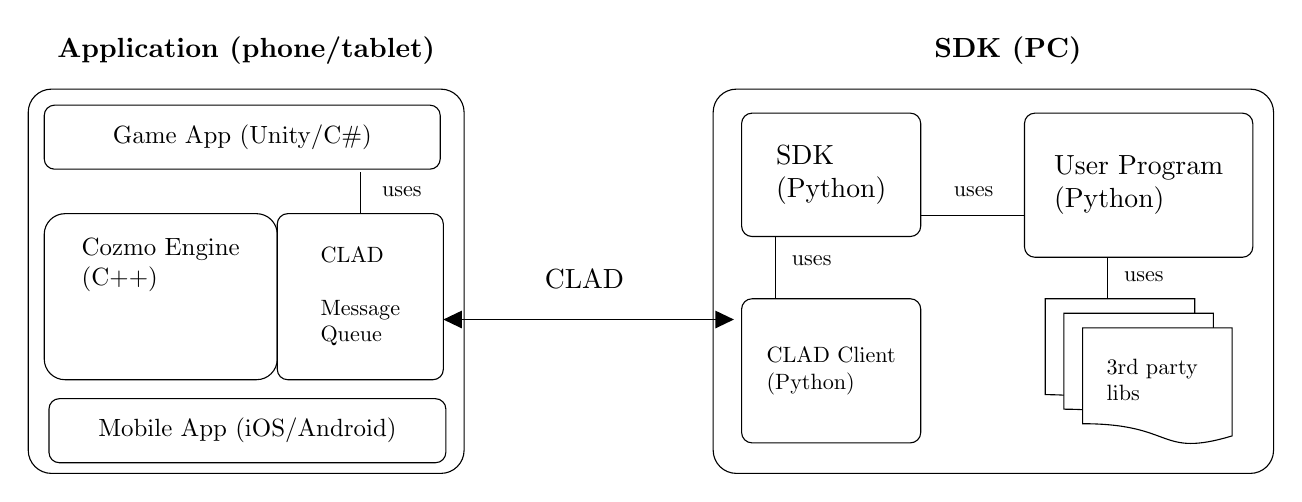
\begin{tikzpicture}[x=0.75pt,y=0.75pt,yscale=-1,xscale=1]
			%uncomment if require: \path (0,466); %set diagram left start at 0, and has height of 466

			%Shape: Rectangle [id:dp01326013235082557] 
			\draw   (353.71,55.57) .. controls (353.71,52.81) and (355.95,50.57) .. (358.71,50.57) -- (435,50.57) .. controls (437.76,50.57) and (440,52.81) .. (440,55.57) -- (440,105) .. controls (440,107.76) and (437.76,110) .. (435,110) -- (358.71,110) .. controls (355.95,110) and (353.71,107.76) .. (353.71,105) -- cycle ;
			%Rounded Rect [id:dp6707545818557623] 
			\draw   (340,50.19) .. controls (340,44.01) and (345.01,39) .. (351.19,39) -- (598.81,39) .. controls (604.99,39) and (610,44.01) .. (610,50.19) -- (610,212.96) .. controls (610,219.13) and (604.99,224.14) .. (598.81,224.14) -- (351.19,224.14) .. controls (345.01,224.14) and (340,219.13) .. (340,212.96) -- cycle ;
			%Shape: Rectangle [id:dp1247876053058975] 
			\draw   (17.71,51.71) .. controls (17.71,48.95) and (19.95,46.71) .. (22.71,46.71) -- (203.5,46.71) .. controls (206.26,46.71) and (208.5,48.95) .. (208.5,51.71) -- (208.5,72.57) .. controls (208.5,75.33) and (206.26,77.57) .. (203.5,77.57) -- (22.71,77.57) .. controls (19.95,77.57) and (17.71,75.33) .. (17.71,72.57) -- cycle ;
			%Shape: Rectangle [id:dp5285084620933563] 
			\draw   (17.71,109) .. controls (17.71,103.48) and (22.19,99) .. (27.71,99) -- (120,99) .. controls (125.52,99) and (130,103.48) .. (130,109) -- (130,169) .. controls (130,174.52) and (125.52,179) .. (120,179) -- (27.71,179) .. controls (22.19,179) and (17.71,174.52) .. (17.71,169) -- cycle ;
			%Shape: Rectangle [id:dp1411259106243823] 
			\draw   (20,193.14) .. controls (20,190.38) and (22.24,188.14) .. (25,188.14) -- (206.21,188.14) .. controls (208.97,188.14) and (211.21,190.38) .. (211.21,193.14) -- (211.21,214) .. controls (211.21,216.76) and (208.97,219) .. (206.21,219) -- (25,219) .. controls (22.24,219) and (20,216.76) .. (20,214) -- cycle ;
			%Rounded Rect [id:dp924085976000878] 
			\draw   (10,50.19) .. controls (10,44.01) and (15.01,39) .. (21.19,39) -- (208.81,39) .. controls (214.99,39) and (220,44.01) .. (220,50.19) -- (220,212.96) .. controls (220,219.13) and (214.99,224.14) .. (208.81,224.14) -- (21.19,224.14) .. controls (15.01,224.14) and (10,219.13) .. (10,212.96) -- cycle ;
			%Shape: Rectangle [id:dp5178962107538444] 
			\draw   (130,104) .. controls (130,101.24) and (132.24,99) .. (135,99) -- (205,99) .. controls (207.76,99) and (210,101.24) .. (210,104) -- (210,174) .. controls (210,176.76) and (207.76,179) .. (205,179) -- (135,179) .. controls (132.24,179) and (130,176.76) .. (130,174) -- cycle ;
			%Straight Lines [id:da3605271488149666] 
			\draw    (170,79) -- (170,99) ;


			%Shape: Rectangle [id:dp18789236199658887] 
			\draw   (490,55.57) .. controls (490,52.81) and (492.24,50.57) .. (495,50.57) -- (595,50.57) .. controls (597.76,50.57) and (600,52.81) .. (600,55.57) -- (600,115) .. controls (600,117.76) and (597.76,120) .. (595,120) -- (495,120) .. controls (492.24,120) and (490,117.76) .. (490,115) -- cycle ;
			%Shape: Rectangle [id:dp06226066777668593] 
			\draw   (353.71,145) .. controls (353.71,142.24) and (355.95,140) .. (358.71,140) -- (435,140) .. controls (437.76,140) and (440,142.24) .. (440,145) -- (440,204.43) .. controls (440,207.19) and (437.76,209.43) .. (435,209.43) -- (358.71,209.43) .. controls (355.95,209.43) and (353.71,207.19) .. (353.71,204.43) -- cycle ;
			%Straight Lines [id:da26247537190243575] 
			\draw    (213,150) -- (347,150) ;
			\draw [shift={(350,150)}, rotate = 180] [fill={rgb, 255:red, 0; green, 0; blue, 0 }  ][line width=0.08]  [draw opacity=0] (8.93,-4.29) -- (0,0) -- (8.93,4.29) -- cycle    ;
			\draw [shift={(210,150)}, rotate = 0] [fill={rgb, 255:red, 0; green, 0; blue, 0 }  ][line width=0.08]  [draw opacity=0] (8.93,-4.29) -- (0,0) -- (8.93,4.29) -- cycle    ;
			%Straight Lines [id:da8910764864061073] 
			\draw    (370,110) -- (370,140) ;


			%Straight Lines [id:da7025332895008514] 
			\draw    (490,100) -- (440,100) ;


			%Flowchart: Multidocument [id:dp4320351285174221] 
			\draw  [fill={rgb, 255:red, 255; green, 255; blue, 255 }  ,fill opacity=1 ] (572,140) -- (500,140) -- (500,186.2) .. controls (545,186.2) and (536,202.86) .. (572,192.08) -- cycle ; \draw  [fill={rgb, 255:red, 255; green, 255; blue, 255 }  ,fill opacity=1 ] (581,147) -- (509,147) -- (509,193.2) .. controls (554,193.2) and (545,209.86) .. (581,199.08) -- cycle ; \draw  [fill={rgb, 255:red, 255; green, 255; blue, 255 }  ,fill opacity=1 ] (590,154) -- (518,154) -- (518,200.2) .. controls (563,200.2) and (554,216.86) .. (590,206.08) -- cycle ;
			%Straight Lines [id:da0995629449951837] 
			\draw    (530,120) -- (530,140) ;



			% Text Node
			\draw (113.11,62.14) node  [scale=0.9] [align=left] {Game App (Unity/C\#)};
			% Text Node
			\draw (73.86,123.71) node  [scale=0.9] [align=left] {Cozmo Engine\\(C++)};
			% Text Node
			\draw (115.61,203.57) node  [scale=0.9] [align=left] {Mobile App (iOS/Android)};
			% Text Node
			\draw (170,139) node  [scale=0.8] [align=left] {CLAD\\\\Message\\Queue};
			% Text Node
			\draw (190,88.5) node  [scale=0.8] [align=left] {uses};
			% Text Node
			\draw (482,20.5) node   [align=left] {\textbf{SDK (PC)}};
			% Text Node
			\draw (115,20.5) node   [align=left] {\textbf{Application (phone/tablet)}};
			% Text Node
			\draw (396.86,80.29) node   [align=left] {SDK\\(Python)};
			% Text Node
			\draw (545,85.29) node   [align=left] {User Program\\(Python)};
			% Text Node
			\draw (396.86,174.71) node  [scale=0.8] [align=left] {CLAD Client\\(Python)};
			% Text Node
			\draw (387.5,121.5) node  [scale=0.8] [align=left] {uses};
			% Text Node
			\draw (465.5,88.5) node  [scale=0.8] [align=left] {uses};
			% Text Node
			\draw (551.5,179) node   [scale=0.8,align=left] {3rd party\\libs};
			% Text Node
			\draw (547.5,129.5) node  [scale=0.8] [align=left] {uses};
			% Text Node
			\draw (278,130.5) node   [align=left] {CLAD};
		\end{tikzpicture}
	}
	\caption[Interaction Application/PC]{Interaction between the mobile application stack and the Python user program. Anki designed a C-like Abstract Data Language (CLAD) to implement the connection between the Cozmo SDK and the Cozmo Engine on the mobile application. This approach puts a decoupling layer between Python interfaces and low-level functions to make prototyping easier and fast-forwarding for developers. \cite{mellon2017cognitive}}
	\label{fig:cozmotear2}
\end{figure}

This approach results in a process method much lighter than the one provided by \textit{Protocol Buffers (Protobuf)} by Google: even then, the main aim of this implementation choice was reducing the network bandwidth.
Taking all arguments into account, CLAD is the protocol used for the interaction between the SDK ant the C++ Engine that allows the developer to not care about the low-level part of the code and to focus on the high-level logic using Python. It is also useful to maintain the same interface for the user even if low-level logic changes occur.

In this case, the CLAD communication messages exploit a wired connection between the mobile device and the computer with a simple USB cable. In this thesis, we used an Android tablet to run the experiments, and for this reason, we used the \textit{Android Debug Bridge (ADB)} to make this exchange possible.
It is a command-line tool included in the \textit{Android SDK Platform-Tools} package that allows the communication between the computer and Android devices. It facilitates many device actions such as installing, debugging apps or running a variety of commands on a device. It is a client-server program that includes three components: it includes a \textit{client} hosted in the development machine, a \textit{daemon (adbd)} which runs the commands on the device as a background process and finally a \textit{server}, a background process in the development machine that manages the communication between the two previous components.

The last step to start programming with Cozmo SDK is to install it in a development machine following the instruction provided by its documentation \footnote{Cozmo SDK Documentation: \href{http://cozmosdk.anki.com/docs/index.html}{http://cozmosdk.anki.com/docs/}}.


\subsection{Why Cozmo?}

Before starting the development of this thesis project, we spent some time analysing the small car market situation in order to find out the right choice for our specific needs. In addition to Anki Cozmo, the ideal alternatives in the self-driving scenario when we started this thesis were \textit{AWS DeepRacer Vehicle} and a customised car implemented from scratch exploiting \textit{Donkey \textregistered
Car library}.

This section part aims to briefly describe the main alternatives to Anki Cozmo listing strengths and weaknesses for each approach to motivate the final choice made.

\subsubsection{AWS DeepRacer}

\textit{AWS DeepRacer} is a platform developed by Amazon to learn and refine machine learning and reinforcement learning algorithms and techniques on AWS DeepRacer vehicle.

The whole ecosystem consists of two main part:
\begin{itemize}
\item \textbf{AWS DeepRacer Car}. It is a 1/18 scale race car developed and built to test reinforcement learning algorithms on a real track. It aims to show how the reinforcement learning model trained in a simulated environment can be conveyed to the real-world by using cameras to view the track and the model to control throttle and steering. It has a lot of interesting specifications under the hood such as Intel Atom \textsuperscript{\textregistered} Processor, 4GB of RAM, an expandable 32GB of storage to accommodate the trained model and a 4-megapixel camera with MJPEG.
\item \textbf{AWS DeepRacer Simulator}. The user can build his models in \textit{Amazon SageMaker} and train, test and iterate the learning process using the racing simulator. It offers an integrated environment hosted on the AWS cloud to experiment and optimise algorithms to apply to the autonomous driving model.
\end{itemize}

There are many advantages in using the DeepRacer stack. It offers an integrated approach where the developer has to focus just on reinforcement learning: indeed, it abstracts a significant part of the software giving the developer the chance to work almost exclusively on the model. It has a growing development community to confront ideas and find solutions through challenging competitions around the world. One of the fundamental aims behind this product is to build up a regulated environment where amateurs and researchers can compare and tests different approaches in solving the autonomous driving task. Therefore it provides a high-performance car where to store the trained model in order to make it independent to the training environment.


On the other hand, one of the main disadvantages of this approach is that it is an Amazon lock-in: the framework provided force developer to use the whole Amazon stack. This fact can be inconvenient economically-wise because of the rates of the Amazon platform that adds to the price of the car, but, above all, because Amazon may have access to all developer implementations and experiments. 

Another not negligible factor was the product release date: Amazon had to release it in July, but, to date, it is not yet available in Italy. Therefore, because of this thesis is focused on the application of reinforcement learning algorithms directly in the real world without the aid of simulators and model, the absence of the physical car was crucial for the final decision.

Another important withdraw consists of the strict correlation between the simulator and the real system: the framework provided by Amazon seems to be suitable only to test reinforcement learning algorithms after the model training in the simulator, but not for the sake of this thesis.

\subsubsection{Donkey\textregistered Car} 

The second important alternative to Cozmo was to develop a small car from scratch using integrated boards such as \textit{RaspberryPi} or \textit{NVIDIA Jetson Nano}, sensors and camera to personalise the device and satisfy specific project needs.
\textit{Donkey\textregistered Car} \footnote{Donkey Car community website: \href{https://www.donkeycar.com}{https://www.donkeycar.com}} is the most popular choice to build a personal self driving toy car. It is an open-source community project powered by volunteers who are interested in build their own self-driving cars. They cooperated to build up a high-level self-driving library written in Python, focusing on enabling fast experimentation and easy contribution. They provide detailed instructions to build a personal Donkey, providing kits or lists of components to use: the whole kit costs among 250-300\$.

It is also possible to install the Donkey library on any RC car to make it self-driving and autonomous. Despite this fact, Donkey developers suggest building the \textit{Donkey2} car, which is a tested hardware and software setup, to avoid problems such as incompatibilities or bugs and make the most out of the presence of a dense community.

The main strength of this choice is the freedom to develop a completely customised car to better suit the needs and requirements of a great set of autonomous driving projects. In the last releases of the library, Donkey developers released a complete sandbox simulator for training a self-driving car. The languages used to develop it are Unity for simulation and Python with Keras and Tensorflow for training. They also provide an OpenAI Gym environment to use with such simulator.

The main weakness of this method consists in the process of building a self-driving car system from scratch. It offers versatility and flexibility in components choice, but the time to devote to building a working system, free from as many bugs as possible would have slowed down the prototyping of the system itself and the whole thesis project. The duration of development is not associated with the process of physically assembling the car because Donkey developers estimate two hours to build the car. The real obstacle consists of the setup of a connection similar to the Cozmo one: it needs to be as stable as possible to make all stack working smoothly in real-time.  

\subsubsection{The final choice}

As easily predictable, the final choice fell on Anki Cozmo. It provides a fast-forwarding SDK ready to be exploited in prototyping a brand new project together with the strictly necessary sensors to perform the reinforcement learning experiments in the real world.
A crucial factor in reaching the final decision was the dimension of the car: as reported before, both Donkey car and Amazon DeepRacer are 1/10 and 1/18 scale race car respectively, while Cozmo is just 5.5cm wide, which results in a ratio of about 1/30. This fact not only makes Cozmo an easily transportable solution to speed up experiments and to restart episodes effortlessly but also a solution that supports the design of a track in a restrict space such as the one in the laboratory of Eurecom.

Therefore, the connection between the development machine and the robot is suitable for implementing an OpenAI Gym environment, and it is similar, at least in the premises, to the distributed off-board computation approach. The main algorithm, the neural network, the reinforcement learning framework and the other cognitive parts are computed and managed by the workstation, instead of being stored in the vehicle as happens in Amazon DeepRacer and Donkey car approaches.

Taking into account the perspective of autonomous cars in the real world, on-board and off-board computation approaches are still under research. With the on-board method, cars have much computational hardware inside in order to manage every aspect of autonomous driving by themselves, but it requires more powerful batteries to counterbalance energy consumption. On the other hand, the connection to off-board computer facilities or the clouds leads to new vectors of attack but also enables companies to monitor the behaviour the vehicle fleet to identify malicious activities early.
To date, both approaches are still under research, and there it is not possible to decree a legitimate winner. For what concerns the thesis, the designed system emulate an off-board approach.

In the end, Cozmo provides plain and straightforward control of the car and a rich Python SDK to use with OpenAI Gym and it is the best trade-off between functionalities and fast-developing. 


\section{PyTorch}

PyTorch \footnote{PyTorch Github Repository: \href{https://github.com/pytorch/pytorch}{https://github.com/pytorch/pytorch}} \cite{paszke2017automatic}  is an open-source machine learning and deep learning library developed by Facebook's AI Research Lab and released to the public in October 2016. The main aim of PyTorch is to provide an intuitive and straightforward framework to develop artificial intelligence projects: two of the main applications to date are computer vision and natural language processing.

The programming languages utilised to develop PyTorch were Python, C++ and CUDA, the parallel computing and API model created by Nvidia to allow software developers and engineers to use CUDA-enabled GPU for general purpose processing. The primary interface provided by the library to the user employs Python, the project where Facebook developers mainly put their efforts. Despite this fact, it also offers a C++ interface. 

PyTorch consists of the following components:
\begin{itemize}
\item \textbf{\texttt{torch}}: PyTorch Tensor library with strong GPU support. It implements interfaces similar to those of the NumPy library. It contains data structures for multi-dimensional tensors and mathematical operations, providing many utilities for efficient serialising tensors and arbitrary types.
\item \textbf{\texttt{torch.autograd}}: the tape-based automatic differentiation library that supports every differentiable operation on tensors available in \texttt{torch}. 
\item \textbf{\texttt{torch.jit}}: this component is a compilation stack that uses TorchScript to create serializable and optimizable models from PyTorch code. This tool allows the user to train models in PyTorch using Python and then export the model in a production environment where Python may be disadvantageous for performance and multi-threading reasons.
\item \textbf{\texttt{torch.nn}}: this component provides a neural networks library that is entirely compatible with \texttt{autograd} and designed for flexibility.
\item \textbf{\texttt{torch.multiprocessing}}: this component is based on the Python multiprocessing library, but it implements memory sharing of torch tensors across processes.
\item \textbf{\texttt{torch.utils}}: it contains many utility functions to better exploits the features of PyTorch.
\end{itemize}

PyTorch provides a NumPy-like experience to interact and manipulate data structures suitable for GPU computation, offering a deep learning research platform which can provide flexibility and speed. These data structures are called \textit{Tensors} and they can be used both on the CPU and the GPU, accelerating the computation thanks to the whole set of functions and manipulators explicitly designed for every scientific computation need. 

PyTorch is not a straightforward binding to an underlying complex C++ framework. The library design focused on establishing Python as the main priority, and for this reason, the user experience is very natural and similar to other important machine learning libraries already present in the package manager.

It is noticeable that PyTorch developers aimed to create an intuitive and linear product to use. To follow this idea, they decided to make PyTorch synchronous to permit the debugger to receive and understand messages and stack traces promptly. This feature translates in a better debugging experience for the end-user.

Beyond these features, one of the traits that distinguish PyTorch from other frameworks is its single way to build neural networks by using a tape-based automatic differentiation.
The majority of deep learning frameworks available in the market, such as TensorFlow, Theano or Caffe, exploits a static approach in structure computation graph creation: they reuse the same layout in the whole program, therefore changing a simple component triggers the regeneration of the graph from scratch.
PyTorch utilises an entirely different approach which is not unique to PyTorch, but it provides one of the fastest implementations: they call it \textit{Tape-Based Autograd}.
This term refers to the reverse-mode automatic differentiation exploited in the framework, which is a technique based on the properties of the chain rule: to calculate the derivative of an output variable w.r.t. any intermediate or input variable, the only requirement is to know the derivatives of its parents and the formula to calculate derivative of primitive expression.
The main improvement that this approach brings is allowing the user to change the network structure on-the-fly without lag or overhead.

\subsection{TensorboardX}

One of the most crucial means that every machine learning researchers need is a tool to visualise and measure data efficiently: this fact is significant because to improve models, projects and results, we need to measure.
However, one of the main problem in PyTorch is the absence of such a tool, specifically designed for the Facebook framework. It can always use powerful tools such as \textit{Matplotlib}, but it offers a synchronous approach that leads to slow down the main program since the primary process has to wait for the data rendering before starting next operations. 

On the other hand, TensorFlow, the most important deep learning alternative to PyTorch developed by Google, provides in its package TensorBoard which is a webserver to serve visualisation of the training progress of the neural network. It can show to the user scalar values, images or text, and it is particularly useful to visualise experimental metrics such as loss and accuracy. The particularity of this tool consists in the fact that it stores these typologies of information asynchronously as events.
The Python script calls specific functions to store information and goes on with the next operation without waiting for its render: that is possible thanks to the decoupling level inserted by this approach between the visualisation and the creation of data. Indeed, Tensorboard operates by opening and reading  TensorFlow events files that contain the summary data generated during experiments. Therefore, it will be the webserver to take care of elaborate data for rendering without bothering the current Python script.

Fortunately, PyTorch can exploit the features of Tensorboard thanks to a library called \textit{TensorboardX} \footnote{TensorBoardX documentation: \href{https://tensorboardx.readthedocs.io/en/latest/index.html}{https://tensorboardx.readthedocs.io/}} that stands for \textit{Tensorboard for X} to highlight developers aim to make Tensorboard available for all deep learning framework.

\subsection{PyTorch vs. TensorFlow}

After the advent of deep learning, many companies decided to put their efforts to design architectures and frameworks to vehiculate this new technology. The two most popular frameworks in this research field are TensorFlow \cite{abadi2016tensorflow} by Google released in 2015 and PyTorch \cite{paszke2017automatic}  by Facebook released in 2017.

Implementing the same neural network in these two frameworks will lead to different results because of the training process has many parameters that depend on the underlying technologies provided by the specific framework. For instance, the training process in PyTorch is enhanced by CUDA GPU usage, while TensorFlow can access to GPU through its GPU acceleration.
The choice between these two frameworks is not straightforward because it depends on the perspective and the needs of the specific projects to develop.
For this reason, this section aims to outline differences between these two libraries without aiming to decree the best one but to motivate the decision to use PyTorch.

\subsubsection{Dynamic versus Static}

The first difference concerns the construction of the computational graph. A computational graph is an abstraction useful to represent the computation process through a direct graph.

In TensorFlow, computational graphs are defined statically, before running the code. The main advantage of this method is allowing parallelism and dependency driving scheduling, features that boost the learning and make it more efficient. This framework communicates with the external world via specific tensors that will be substituted by input data at runtime. 
Only with TensorFlow 2.0, Google decided to implement dynamic computational graph in its product, but its stable version was released after the start of this thesis.

As mentioned above, PyTorch approach to computational graphs is dynamic. This characteristic means that the graph is built incrementally at runtime without using particular data structures as placeholders. This feature supports projects where the author needs to change the computational graph on-the-fly avoiding the application restart. In this sense, PyTorch is more pythonic than TensorFlow.

\subsubsection{Distributed Training}

Another key feature is the distributed training and data parallelism. PyTorch offers native support for asynchronous execution from Python, and then it could improve performances. On the other hand, TensorFlow needs more efforts to allow distributed training: the developer must fine-tune every computation to make it running on a specific device. Both frameworks offer the same opportunities in these terms. However, TensorFlow needs more effort to make things work.

\subsubsection{Visualisation}

As discussed in the previous section, TensorFlow exploits TensorBoard to provide all tools that machine learning researcher needs to visualise learning and keep track of the training process. Facebook researchers developed \textit{Visdom} for this purpose, but it provides very minimalistic and limited features compared to the ones offered by TensorBoard. As reported before, it is possible to use TensorBoard with PyTorch thanks to the library TensorBoardX.

\subsubsection{Production Deployment}

For what concerns the deployment of trained models into production, TensorFlow offers the best service via \textit{TensorFlow serving}, a framework that offers and uses REST Client API.
The production deployment in PyTorch improved from its early releases, but, currently, it does not provide a framework to deploy the trained models on the web: the developers must use Flask or Django as backend server to provide the right environment to exploit the model.

\subsubsection{Conclusions}

Considering all the points explained in this section, we decided to utilise PyTorch for this project, but it is noticeable that there is no winner in this comparison.

Both frameworks have strengths and weaknesses that depends on the specific applications where we would use them.
TensorFlow is a mature and robust tool, notably suggested for production and AI-related products. Although it needs some time to get the developer used to its programming approach and, at least at the start of this thesis project,  it supports only static computational graph methods. On the other side, PyTorch is an efficient and young framework with a large community and which provides dynamic computational graphs and is more Python friendly. Therefore, it is especially recommended for research-oriented developers.
	\chapter{Design of the control system} \label{ch4}

In the previous chapters, we outlined deep reinforcement learning fundamentals and the most critical underlying concepts, and then we discussed the choice made about the technologies to use as baselines for our experiments. The decision fell on Anki Cozmo because of the high-quality SDK provided to developers and the versatility and flexibility provided by PyTorch, especially in a research context.

The next step in this thesis is the merge of reinforcement learning theory with the tool presented previously. Indeed, this chapter aims to describe this merge process that results in the design of the control system for reinforcement learning experiments with Anki Cozmo. The work presented in this section represents one of the contributions of our thesis and the necessary step to start reinforcement learning experiments.

The outline of the whole ecosystem with the description of interfaces, frameworks and technologies used occupies the first section of the chapter. This part also comprehends a discussion about DDPG \cite{lillicrap2015continuous} and SAC \cite{haarnoja2018soft, haarnoja2018alg} implementation with references to the choice made in terms of hyper-parameters and problems faced.

The second part of the chapter aims to describe the implementation of Anki Cozmo OpenAI Gym environment from the problem formalisation as MDP to the implementation of human-robot interaction.

In the final section of this chapter, the design and setup of the real track will be discussed together with a discussion about the problems faced and the choice made to overcome them.

\section{Outline of the system}

The development of the control system for Anki Cozmo was the main contribution of the thesis, together with the implementation of DDPG and SAC algorithm. The main aim of this work was to create an OpenAI Gym environment capable of interacting with a robot in the real world, not just through the usage of a simulator. OpenAI Gym usually provides plain and straightforward interfaces to interact with simulated environments: we decided to exploit these functions to allow the application of reinforcement learning algorithm directly in the real-world decision of the robot.

The fundamental source of inspiration to develop this control system was \cite{kendall2018learning,kendall2019learning}. This publication represents, as its authors reported,  the first reinforcement learning self-driving experiment where a car learned to drive through the application of a reinforcement learning algorithm, by trial and error. They first trained the model exploiting Deep Deterministic Policy Gradient (DDPG) in a simulator for many epochs and, after this learning process, they managed to transfer the knowledge acquired in the simulator in real-world experiments. 

We decided to export and implement these ideas in our project, adapting them to the specificities and particularities of the Cozmo setup. The resulting system can be summed up by \vref{fig:system} which provide a schematic overview of every technology employed and the interaction among them.
This section aims to describe as clearly as possible all the components of the control system we designed.

\tikzset{every picture/.style={line width=0.75pt}} %set default line width to 0.75pt        

\begin{figure}
	\tikzset{every picture/.style={line width=0.75pt}} %set default line width to 0.75pt    
	\centering
	\scalebox{0.85}{


		\tikzset{every picture/.style={line width=0.75pt}} %set default line width to 0.75pt        

	\begin{tikzpicture}[x=0.75pt,y=0.75pt,yscale=-1,xscale=1]
		%uncomment if require: \path (0,438); %set diagram left start at 0, and has height of 438

		%Image [id:dp06991158821872456] 
		\draw (239.75,55) node  {
\includegraphics[width=115.13pt,height=52.5pt]{img/python.png}};
		%Image [id:dp3729269645681633] 
		\draw (240.25,198.5) node  {
\includegraphics[width=46.88pt,height=50.25pt]{img/gym.png}};
		%Image [id:dp09149607927009118] 
		\draw (94.75,200.91) node  {
\includegraphics[width=124.13pt,height=25.37pt]{img/pytorch.png}};
		%Image [id:dp30806594376010465] 
		\draw (351.92,200) node  {
\includegraphics[width=40.38pt,height=52.5pt]{img/flask.png}};
		%Straight Lines [id:da3933293266418665] 
		\draw    (239.98,93) -- (239.52,159) ;
		\draw [shift={(239.5,162)}, rotate = 270.4] [fill={rgb, 255:red, 0; green, 0; blue, 0 }  ][line width=0.08]  [draw opacity=0] (8.93,-4.29) -- (0,0) -- (8.93,4.29) -- cycle    ;
		\draw [shift={(240,90)}, rotate = 90.4] [fill={rgb, 255:red, 0; green, 0; blue, 0 }  ][line width=0.08]  [draw opacity=0] (8.93,-4.29) -- (0,0) -- (8.93,4.29) -- cycle    ;
		%Straight Lines [id:da24057878811893751] 
		\draw    (167.75,200.25) -- (203.75,200.25) ;
		\draw [shift={(206.75,200.25)}, rotate = 180] [fill={rgb, 255:red, 0; green, 0; blue, 0 }  ][line width=0.08]  [draw opacity=0] (8.93,-4.29) -- (0,0) -- (8.93,4.29) -- cycle    ;
		\draw [shift={(164.75,200.25)}, rotate = 0] [fill={rgb, 255:red, 0; green, 0; blue, 0 }  ][line width=0.08]  [draw opacity=0] (8.93,-4.29) -- (0,0) -- (8.93,4.29) -- cycle    ;
		%Straight Lines [id:da10061083103025648] 
		\draw    (283.75,199.58) -- (318.5,199.58) ;
		\draw [shift={(321.5,199.58)}, rotate = 180] [fill={rgb, 255:red, 0; green, 0; blue, 0 }  ][line width=0.08]  [draw opacity=0] (8.93,-4.29) -- (0,0) -- (8.93,4.29) -- cycle    ;
		\draw [shift={(280.75,199.58)}, rotate = 0] [fill={rgb, 255:red, 0; green, 0; blue, 0 }  ][line width=0.08]  [draw opacity=0] (8.93,-4.29) -- (0,0) -- (8.93,4.29) -- cycle    ;
		%Image [id:dp8556439958741602] 
		\draw (567,186) node  {
\includegraphics[width=52.5pt,height=52.5pt]{img/user.png}};
		%Straight Lines [id:da26821981951432505] 
		\draw    (385.5,184.58) -- (499.5,184.58) ;
		\draw [shift={(502.5,184.58)}, rotate = 180] [fill={rgb, 255:red, 0; green, 0; blue, 0 }  ][line width=0.08]  [draw opacity=0] (8.93,-4.29) -- (0,0) -- (8.93,4.29) -- cycle    ;

		%Straight Lines [id:da7643998387312995] 
		\draw    (388.5,214.58) -- (412.5,214.58) -- (500.5,214.58) ;

		\draw [shift={(385.5,214.58)}, rotate = 0] [fill={rgb, 255:red, 0; green, 0; blue, 0 }  ][line width=0.08]  [draw opacity=0] (8.93,-4.29) -- (0,0) -- (8.93,4.29) -- cycle    ;
		%Straight Lines [id:da5051570254396728] 
		\draw    (240.5,256) -- (240.5,278) ;
		\draw [shift={(240.5,281)}, rotate = 270] [fill={rgb, 255:red, 0; green, 0; blue, 0 }  ][line width=0.08]  [draw opacity=0] (8.93,-4.29) -- (0,0) -- (8.93,4.29) -- cycle    ;
		\draw [shift={(240.5,253)}, rotate = 90] [fill={rgb, 255:red, 0; green, 0; blue, 0 }  ][line width=0.08]  [draw opacity=0] (8.93,-4.29) -- (0,0) -- (8.93,4.29) -- cycle    ;
		%Rounded Rect [id:dp9694318857670313] 
		\draw   (2,25.5) .. controls (2,15.28) and (10.28,7) .. (20.5,7) -- (464,7) .. controls (474.22,7) and (482.5,15.28) .. (482.5,25.5) -- (482.5,300.5) .. controls (482.5,310.72) and (474.22,319) .. (464,319) -- (20.5,319) .. controls (10.28,319) and (2,310.72) .. (2,300.5) -- cycle ;
		%Image [id:dp9562999520117128] 
		\draw (99,377) node  {
\includegraphics[width=52.5pt,height=52.5pt]{img/tablet.png}};
		%Straight Lines [id:da22030012036466173] 
		\draw    (98.5,295) -- (186.5,295) ;
		\draw [shift={(189.5,295)}, rotate = 180] [fill={rgb, 255:red, 0; green, 0; blue, 0 }  ][line width=0.08]  [draw opacity=0] (8.93,-4.29) -- (0,0) -- (8.93,4.29) -- cycle    ;

		%Straight Lines [id:da28839463654139263] 
		\draw    (98.5,295) -- (98.5,339) ;
		\draw [shift={(98.5,342)}, rotate = 270] [fill={rgb, 255:red, 0; green, 0; blue, 0 }  ][line width=0.08]  [draw opacity=0] (8.93,-4.29) -- (0,0) -- (8.93,4.29) -- cycle    ;

		%Straight Lines [id:da2120925552884272] 
		\draw  [dash pattern={on 0.84pt off 2.51pt}]  (154.75,380.58) -- (473.5,380.58) ;

		\draw [shift={(151.75,380.58)}, rotate = 0] [fill={rgb, 255:red, 0; green, 0; blue, 0 }  ][line width=0.08]  [draw opacity=0] (8.93,-4.29) -- (0,0) -- (8.93,4.29) -- cycle    ;
		%Image [id:dp7151280650926004] 
		\draw (535.32,366) node  {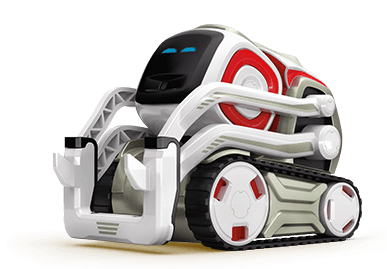
\includegraphics[width=96.27pt,height=69.12pt]{img/cozmo.png}};
		%Straight Lines [id:da948112813701837] 
		\draw  [dash pattern={on 0.84pt off 2.51pt}]  (151.75,402.58) -- (470.5,402.58) ;
		\draw [shift={(473.5,402.58)}, rotate = 180] [fill={rgb, 255:red, 0; green, 0; blue, 0 }  ][line width=0.08]  [draw opacity=0] (8.93,-4.29) -- (0,0) -- (8.93,4.29) -- cycle    ;

		%Image [id:dp8991970614844648] 
		\draw (332,113) node  {
\includegraphics[width=36pt,height=36pt]{img/tensorflow.png}};
		%Straight Lines [id:da8686562029937168] 
		\draw    (257.5,118) -- (297.5,118) ;
		\draw [shift={(300.5,118)}, rotate = 180] [fill={rgb, 255:red, 0; green, 0; blue, 0 }  ][line width=0.08]  [draw opacity=0] (8.93,-4.29) -- (0,0) -- (8.93,4.29) -- cycle    ;

		%Straight Lines [id:da7903500333471788] 
		\draw    (257.5,118) -- (257.5,165) ;


		%Straight Lines [id:da017309376357115047] 
		\draw    (557.15,117.91) -- (557.15,93) ;
		\draw [shift={(557.15,90)}, rotate = 450] [fill={rgb, 255:red, 0; green, 0; blue, 0 }  ][line width=0.08]  [draw opacity=0] (8.93,-4.29) -- (0,0) -- (8.93,4.29) -- cycle    ;

		%Straight Lines [id:da46777924457369235] 
		\draw    (557.15,117.91) -- (453.67,117.91) ;


		%Image [id:dp9871015067821471] 
		\draw (559,44) node  {
\includegraphics[width=42pt,height=42pt]{img/analysis.png}};

		% Text Node
		\draw (569,227) node  [font=\footnotesize] [align=left] {Human-Robot Interaction};
		% Text Node
		\draw (435,175) node  [font=\footnotesize] [align=left] {Image};
		% Text Node
		\draw (436,204) node  [font=\footnotesize] [align=left] {Commands};
		% Text Node
		\draw (114,22) node   [align=left] {\textbf{Development Machine}};
		% Text Node
		\draw    (196.5,282.5) -- (287.5,282.5) -- (287.5,307.5) -- (196.5,307.5) -- cycle  ;
		\draw (242,295) node   [align=left] {Cozmo SDK};
		% Text Node
		\draw (100,423) node   [align=left] {\textbf{Android Device}};
		% Text Node
		\draw (120,276) node   [align=left] {{\footnotesize ADB}};
		% Text Node
		\draw (323,420) node   [align=left] {Wi-Fi Connection};
		% Text Node
		\draw (536,420) node   [align=left] {\textbf{Cozmo}};
		% Text Node
		\draw (319,370) node  [font=\footnotesize] [align=left] {Image};
		% Text Node
		\draw (320,394) node  [font=\footnotesize] [align=left] {Commands};
		% Text Node
		\draw (396,119) node   [align=left] {TensorBoard};
		% Text Node
		\draw (559,75) node  [font=\footnotesize,] [align=left] {Data Analysis};
		% Text Node
		\draw (241,242) node   [align=left] {OpenAI Gym};


	\end{tikzpicture}
	}
	\caption[Interaction Human/Robot]{Interaction between the user and Anki Cozmo. The main Python script utilises OpenAI Gym for the reinforcement learning component and PyTorch for the deep learning one. The user can interact with the flow of the system through a simple web app implemented using HTML, CSS, JS that communicates with a Flask backend. This component interacts directly with OpenAI Gym and the Cozmo SDK to provide information for the user (e.g.\ images, learning information) and the robot (e.g.\ commands). The last component consists in TensorBoard thanks to the script can store results that can be retrieved later by the user.}
	\label{fig:system}
\end{figure}

\subsection{Human-Robot Interaction}

It is noticeable that the simulator can undoubtedly be programmed to understand when the car is outside the track. In a reinforcement learning scenario, this fact facilitates the restarting procedure for an episode: the developer has to bind some events or actions to a process that stops the current episode, put the car on the road again and starts the next experiment. In the real world, the situation is more complicated because there are more variables to take into account: the most critical factor is that the failure of an episode in the simulator has no threats or costs, while real-world experiments failures could lead to high costs. Despite this point, the application of such experiment typology in a real environment instead of a mere simulation represents an exciting challenge that could bring reinforcement learning to the next level. In order to make experiments as safe as possible, the authors of \cite{kendall2018learning,kendall2019learning} implemented a self-driving system designed explicitly for reinforcement learning experiments where the car driver has the faculty of stopping the car when it is going to run off the road or in a dangerous situation and relocating it in the nearest safe position to start the next learning episode.

For this reason, we firstly implemented a straightforward interface using a web app implemented using plain HTML, CSS and Javascript for the frontend and Flask as backend. The aim of this application is allowing user interaction with Cozmo and Flask represented the right choice to allow the communication between this interface and the OpenAI Gym environment. The user can see a sort of live streaming from the camera of Cozmo directly in the web app and can send commands to the robot through the computer keyboard. Just as example

In this context, the human-robot interaction has a crucial role in the learning process because it is the source of all improvements and flaws of the learning process: the robot learns which actions are worthy and which are not, but the human is the one who decides the correctness of each action, carrying its unconscious bias in the algorithm. We will discuss the experiments and their results thoroughly in \vref{ch5,ch6}.




% \todomacaluso{
% 	\begin{itemize}
% 		\item Introduction to the chapter
% 		\item General description of the control systems with a diagram representing all the technologies involved.
% 		\item Setup of the algorithms (DDPG, SAC)
% 		      \begin{itemize}
% 			      \item We decided to rewrite both algorithms without using libraries directly. The first motivation was didactical, implementing from scratch is helpful to understand the practical implementation of the algorithm better, but also to make it possible to implement the singularity of the real Cozmo environment.
% 			      \item The interaction with OpenAI Gym and PyTorch
% 			      \item Discussion about Hyper-Parameters and the problems faced in the real world situation in the selection of these parameters.
% 		      \end{itemize}
% 		\item Setup and implementation of CozmoEnv
% 		      \begin{itemize}
% 			      \item Technologies used to implement the interaction between the Cozmo SDK and OpenAI Gym.
% 			      \item Differences from the simulated environment caused by the need for direct human interaction.
% 			      \item Implementation of human interaction in the system.
% 		      \end{itemize}
% 		\item Setup of the real Environment
% 		      \begin{itemize}
% 			      \item The Track design
% 			      \item Analysis of the problems:
% 			            \begin{itemize}
% 				            \item Reflection
% 				            \item Background and Horizon
% 			            \end{itemize}
% 			      \item (Single Line Track)
% 		      \end{itemize}
% 	\end{itemize}
% }

% \section{The track}

% The design and training of a good driving model cannot go beyond the construction and design of the road. For this reason, some time was spent searching the better way to build a path where to train Cozmo.
% This section aims to present the central concept and decisions made about the design of the track for the experiments, starting from the materials used, up to the description of the dimensional choices applied.

% \subsection{Track requirements}

% It is essential to explain the primary needs of the road before proceeding with the description of the choices made.

% Firstly, the track needs to be easily transportable to allow various attempt with different locations and environmental conditions that could affect the training phase. In particular, it is necessary to use a material less reflective as possible to avoid problems during the learning process.
% Another crucial factor is the dimension of the lane, which must reproduce an environment similar to the real one. It can be done analyzing the ratio of the size of a vehicle to the width of a road. On average, a family car is about $160$-$170$cm large, while a lane width can vary between $275$cm and $375$cm. Cozmo width is about $5.5$cm, which results in a ratio of $1/30$. Therefore, the scaled lane must be between $9$cm and $12.5$cm.

% \subsection{Track design and materials}

% The first choice to make is the one about the type of material to use as terrain for the track. The first choice was the black floor of the Data Science laboratory of Eurecom. It was useful only during the initial design and development of the control system to build small pieces of track in which testing functionalities. This solution had numerous drawbacks such as the impracticality to transport and high light reflection. 

% The following list provides a brief report of the various solutions taken into account during the thesis, together with an analysis of advantages and drawbacks.

% \begin{itemize}
% 	\item \textit{Covering fabric}: this material is easily transportable, but it has a high light reflection, and its structure is prone to make wrinkles and dunes challenging to remove.
% 	\item \textit{Tar paper}: this solution slightly diminished the reflection problem compared to the previous choice, but the material was fragile and with the same drawbacks of the covering fabric.
% 	\item \textit{Cotton fabric}: this solution offers an easily  transportable material with reduced light reflection where it is easy to remove wrinkles and dunes.
% \end{itemize}

% Summing up, it is noticeable from this analysis that the cotton fabric provides the right trade-off among all requirements reported before.

% The structure of the road is also composed by the lane. The implementation of this part was done using a simple paper tape of width equal to $2.5$cm. As described in the beginning of this section, the width of the lane must be between $9$cm and $12.5$cm to provide a context similar to the real one. Because of the narrow and limited angle of vision provided by Cozmo camera, $10$cm-width was set: positioning the tape with a distance greater than $10$cm would result in a great part of the tape outside the view of the camera.
	\chapter{Experimental results} \label{ch:ch5}

In the previous chapters, we described the reinforcement learning control system we designed, together with an analysis of the solutions we proposed for the problems we faced during the development process.
Indeed, this process has not been free from difficulties, both of implementation level and parameter optimisation.
After completing the design of this architecture, our second goal was to look for an algorithm that could better adapt to a real context, exceeding the limits set by DDPG.
The ideal would have been to find an algorithm altogether parameter agnostic: an enabling feature to achieve excellent performance regardless of the specific configuration.
During our research we came across the SAC algorithm and, after a careful analysis of the paper and having understood the considerations made by the authors about SAC real-world applications, we thought it might be the right choice to get better performance than the DDPG experiments.
For this reason, this chapter aims to present a detailed comparison of the experiments carried out on both algorithms.

The first section of this chapter focuses on the experimental methodology.
It will be an opportunity to describe the hardware of the development machine we used for the experiments and present in a more schematic and precise way the OpenAI Gym environments on which we will apply the algorithms.
We speak in the plural, because we have decided to report both the experiments performed on \textit{Pendulum-v0} environment, and those carried out with Anki Cozmo in the real world using the architecture we built.
This part will also contain a brief analysis of how reinforcement learning experiments are assessed to date.
For this segment, we took inspiration by \cite{henderson2018deep}, an exciting publication where the authors investigated reproducibility challenges, proper experimental techniques, and reporting procedures of modern deep reinforcement learning to draw up guidelines from which to start in order to obtain better reports, not so much from the result perspective, but from how they are reported.

The second and third sections of this chapter will, therefore, be devoted respectively to the two types of environments used.
We have shown all the useful graphs in order to analyse and to comment on the obtained results.

\section{Experimental Methodology}

This pre-trial section is essential to understand better the tasks we tried to get the reinforcement learning algorithms to solve and what approach we used to evaluate experiments results.

\subsection{Hardware and Software details}

In order to carry out the experiments contained in this chapter, we have made use of a personal laptop.
We chose this solution because the machine has excellent specifications to support the computational power required by the experiments both in terms of GPU and RAM.

Despite these considerations, we still had problems in terms of RAM memory. This type of experiment requires a very large experience memory replay to allow optimal batch extraction. Despite the large amount of RAM present and the reduction of the size of the input image, we were still forced to reduce the maximum size of the replay memory to complete the experiments.

We collected the essential information about hardware and software that we have used to perform experiments in \vref{table:hw_spec,table:sw_spec}.

\begin{table}[!h]
	\centering
	\caption{Development Machine Hardware Specifications}
	\label{table:hw_spec}
	\begin{tabular}{@{}lllll@{}}
		\toprule
		\textbf{Component} & \textbf{Details}                                                                      \\
		\midrule
		\textbf{Laptop}    & Dell Inspiron 15 7559                                                                 \\\midrule
		\textbf{CPU}       & Intel\textsuperscript{\textregistered} Core\textsuperscript{\texttrademark} i7-6700HQ \\
		                   & \# of Cores: 4                                                                        \\
		                   & \# of Threads: 8                                                                      \\
		                   & Processor Base Frequency: 2.60 GHz                                                    \\
		                   & Max Turbo Frequency: 3.50 GHz                                                         \\\midrule
		\textbf{GPU}       & NVIDIA GeForce GTX 960M                                                               \\
		                   & CUDA Cores: 640                                                                       \\
		                   & Memory: 4GB GDDR5, 2500 MHz                                                           \\\midrule
		\textbf{RAM}       & 12GB DDR3L, 1600 MHz                                                                  \\
		\bottomrule
	\end{tabular}
\end{table}

\begin{table}[!h]
	\centering
	\caption{Development Machine Software Specifications}
	\label{table:sw_spec}
	\begin{tabular}{@{}lllll@{}}
		\toprule
		\textbf{Component}        & \textbf{Details}                   \\
		\midrule
		\textbf{Operating System} & Ubuntu 18.04.3 LTS (Bionic Beaver) \\\midrule
		\textbf{Python}           & v.3.6.8                            \\\midrule
		\textbf{PyTorch}          & v.1.4.0                            \\\midrule
		\textbf{OpenAI Gym}       & v.0.15.4                           \\
		\bottomrule
	\end{tabular}
\end{table}

\subsection{Pendulum-v0 Environment}

OpenAI Gym \textit{Pendulum-v0} environment formalise the inverted pendulum swing-up problem, a classic problem in the control literature. In this version of the problem, the pendulum starts in a random position, and the goal is to swing it up so it stays upright.

We have also decided to include in this thesis the experiments we have carried out on this simulated environment, because the results obtained and the problems faced were essential to have a more prepared approach to deal with the real-world experiment and the environment we designed for Cozmo.

\begin{figure}[ht!]
	\centering
	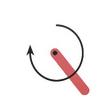
\includegraphics[height=0.2\paperwidth]{img/pendulum.png}
	\caption[Frame of Pendulum-v0 environment]{Frame of Pendulum-v0 environment. We decided to use a set of two subsequent 64$\times$64 images.}
	\label{fig:pendulum}
\end{figure}

\subsubsection{Observation}

The original implementation of this environment is based on an state represented by a \texttt{Box(3)} type, a data structure defined by OpenAI Gym that extends functionalities of a standard array. It contains values related to the current angle of the pendulum as described in \vref{table:pendulum_obs}.

Since the goal of our thesis was to apply DDPG and SAC to a problem such as the autonomous driving one where input data is composed of images, we decided to build a wrapper (\texttt{gym.ObservationWrapper}) for the original environment in order to receive observations as raw pixels. In this way we could apply the same considerations and the same convolutional neural network that we used in the Cozmo environment.

We have started many experiments on this environment to find the most suitable number of images to use as a state, looking for a trade-off between the algorithm’s needs and the space constraints imposed by the hardware we used. The agent revealed instability using a single frame, while leading to excellent results using two images. Finally, for space issues, we decided to resize the image to 64$\times$64 pixels.

A sample screenshot of the environment in action is shown in \vref{fig:pendulum}.

\begin{table}[!h]
	\centering
	\caption{Original Observation \texttt{Pendulum-v0} environment}
	\label{table:pendulum_obs}
	\begin{tabular}{@{}lllll@{}}
		\toprule
		Index & Observation    & Min    & Max    \\ \midrule
		0     & cos($\theta$)  & $-1.0$ & $+1.0$ \\
		1     & sin($\theta$)  & $-1.0$ & $+1.0$ \\
		2     & $\dot{\theta}$ & $-8.0$ & $+8.0$ \\
		\bottomrule
	\end{tabular}
\end{table}

\subsubsection{Actions}

The actions that the agent can perform within this environment are described through a \texttt{Box(1)} object containing only one element. This value corresponds to the joint effort, which allows the agent to swing the pendulum. The action space has been maintained also in the modified environment.

\begin{table}[!h]
	\centering
	\caption{Pendulum-v0 Actions }
	\label{mountain_action}
	\begin{tabular}{@{}lllll@{}}
		\toprule
		Index & Action       & Min    & Max    \\ \midrule
		0     & Joint effort & $-2.0$ & $+2.0$ \\
		\bottomrule
	\end{tabular}
\end{table}

\subsubsection{Reward}
The reward for each timestep $t$ is given by \[r_t = -(\theta_t^2 + 0.1 \dot{\theta}^2 + 0.001 a_t^2)\]
where theta is normalized between $-\pi$ and $\pi$. Therefore, the lowest cost is $-(\pi^2 + 0.1*8^2 + 0.001*2^2) = -16.2736044$, and the highest cost is $0$. In essence, the goal is to remain at zero angle (vertical), with the least rotational velocity, and the least effort.
The reward design has been maintained also in the modified environment.

\subsubsection{Starting State}

The initial state of the environment in question is chosen randomly.
Two values are extracted: the first is an angle between  $-\pi$ to $\pi$, the second is a speed between -1 and 1.
A zero angle corresponds to the standing pendulum.

\subsubsection{Episode Termination}

OpenAI Gym documentation does not specify a particular episode termination for this environment: the choice is left to the user.
In our case, after some attempts, we decided to set a limit value of 200 steps for each episode.

\subsubsection{Solved Requirements}

Also in this case, OpenAI Gym documentation does not specify any indications in order to understand whether an episode has been solved.
Indeed, \textit{Pendulum-v0} is an unsolved environment, which means it does not have a specified reward threshold at which it is considered correctly completed.

\subsection{CozmoDriver-v0 Environment}

\textit{CozmoDriver-v0}, the reinforcement learning environment we implemented, is one of the contribution of this thesis.
This section aims to present as schematically as possible the basic parameters that characterize the environment we have designed.
Further details on the implementation choices, problems encountered and solutions we have adopted to solve them are available in \vref{ch:ch4}.

\subsubsection{Observation}

The observations we decided to use in \textit{CozmoDriver-v0} are the same as those we exploited in the \textit{Pendulum-v0} environment.
In fact, our agent will obtain, for each action carried out, a queue composed of two images from the front camera of Cozmo resized to 64x64 pixels.
As in the previous environment, we decided to resize the images obtained in order to remain within the limits placed by the RAM memory available in the development machine.

The first image represents the state before the action, while the second represents the consequences of the action taken.
The number of images was set to two after performing some experiments on \textit{Pendulum-v0} environment that revealed instability in the use of a single image.
We decided to limit ourselves to two images, as we would increase the size of a single entry in replay memory by adding more of them.
This choice would require a counterbalance that would materialize in the decrease of the maximum size of replay memory.

As we mentioned in \vref{ch:ch3}, Anki Cozmo has a front camera inserted inside its tilting head and one forklift.
In order to obtain more valuable images for our experiments we decided to tilt the head as much as possible down and raise the forklift: in this way the image is focused as much as possible on the lane, leaving everything that could distract the learning process outside the view.

An example of two subsequent frame received by Cozmo is available in \vref{fig:cozmo_frames}.
\begin{figure}

	\begin{minipage}[t]{0.5\linewidth}
		\centering
		
\includegraphics[height=0.25\paperwidth]{img/cozmo_frame_1.jpg}
	\end{minipage}
	\begin{minipage}[t]{0.5\linewidth}
		\centering
		
\includegraphics[height=0.25\paperwidth]{img/cozmo_frame_2.jpg}
	\end{minipage}

	\caption[Example of two subsequent frame of CozmoDriver-v0]{An example of a two subsequent frame of CozmoDriver-v0 environment. We decided to resize the image returned by Cozmo to 64$\times$64 for memory reason: a higher resolution would lead to a further decrease in experience replay memory.}
	\label{fig:cozmo_frames}
\end{figure}

\subsubsection{Actions}

We have already discussed in \vref{subsubsec:mdp_form} the decisions taken to implement the management of actions within the environment that we have built.

To describe the actions that the agent can perform within this environment, we used a \texttt{Box(2)}. The first value of this object corresponds to the desired speed, while the second one represent the steering wheel position. \Vref{table:cozmo_actions} describes schematically this object.

\begin{table}[!h]
	\centering
	\caption{CozmoDriver-v0 Actions}
	\label{table:cozmo_actions}
	\begin{tabular}{@{}lllll@{}}
		\toprule
		Index & Action                        & Min    & Max    \\ \midrule
		0     & Desired Speed ($v$)           & $0.0$  & $+1.0$ \\
		1     & Steering Wheel Position ($w$) & $-1.0$ & $+1.0$ \\

		\bottomrule
	\end{tabular}
\end{table}

\subsubsection{Reward}

The reward we chose for our experiment was the second one provided by \vref{subsubsec:mdp_form}.
The decision has fallen on the \textit{Lane Distance Reward} because it describes with simplicity the final goal of the task, but above all because it allows the user to have a direct counterproof of the effectiveness of the algorithm, by matching the reward to the distance travelled.
\Vref{eq:reward_fun} reports the calculation that is executed to every timestep to calculate the reward to the carried out action.
$c$ is the time expressed in seconds between one action and the next one, imposed as system constant, while $v_t$ is the desired speed taken by the current action expressed in millimetres per second.

\begin{equation}
	\label{eq:reward_fun}
	r_t = v_t \cdot c
\end{equation}

\subsubsection{Starting State}

The starting state position of the system is not constant, but changes from episode to episode.
This approach was preferred over the one with a fixed starting position for two simple reasons:
\begin{itemize}
	\item Reduces the path that has to be traveled by the robot in order to be able to reposition, speeding up the experiments as it saves more battery.
	      In this approach, the robot is repositioned on the road closest to where the previous episode ended.
	\item It allows the agent to accumulate experiences that do not always refer to the same road segment.
	      With this methodology, the experiences will most always begin and end in different states, leading the agent to put more effort in generalization.
\end{itemize}

The episode starts as soon as the user receives the start signal.

\subsubsection{Episode Termination}

The episode ends when the robot goes off the road or reaches a a dangerous situation.
Even this time, the episode ends when the user receives the stop sign.

\subsubsection{Solved Requirements}

We have not provided a well-defined parameter to understand whether the task has been solved or not, because it depends on the path and the particular needs of the programmer.
Potentially the episode could last forever if the robot could learn to run an entire circuit.

No mechanism has been implemented to communicate to the robot that the episode ended in a positive way.
For this reason, we suggest to apply this environment to circuits and not paths where beginning and end do not coincide.

In our case, the route used is almost 3 meters long.
So we decided to use this value as a target to reach to determine the resolution of the task.

\subsection{Measuring Performance}

In recent years, we have witnessed the rapid growth of interest in deep reinforcement learning by the entire scientific community.
This growth has led to an increase in experiments and work on this subject, which are often easily available.
However, reproducing reinforcement learning experiments is not always as intuitive and straightforward as expected.
Often, the measurements reported by papers and studies of this kind are difficult to interpret due to the non-determinism inherent in most environments in which these algorithms are applied.
Without appropriate and meaningful metrics accompanied by standardization in presenting the results, it becomes difficult to determine conclusively the improvements made to the-state-of-the-art.

Going through the literature, it is noticeable that reinforcement learning algorithms are often evaluated by presenting tables and graphs showing cumulative average rewards or the maximum reward achieved on a pre-set number of timesteps.
But the combined features of environments and algorithms make these values typically inadequate for fair comparison.
This is due to the fact that there are numerous factors that come into play, such as seeds and trials that lead to different performances and that do not contribute to make clearer the actual performance of an algorithm.
However, when these are accompanied by confidence intervals, based on a fairly large number of attempts, then there are the premises to make decisions and formulate more informed considerations.

Once again, however, we have been forced to come to terms with reality.
We were able to produce as honest and specific an analysis as possible regarding experiments on \textit{Pendulum-v0}.
In this case, we could easily repeat the experiments 10 times for each algorithm, so that we could report graphs containing more useful information, such as confidence margins.

On the other hand, experiments with Cozmo took a much larger number of episodes before starting to show the first improvements.
We managed to maintain an average of just under 750 episodes per day: this underlines how difficult it was to get to conclude even a single experiment.
For this experiment, we reported the results obtained without any confidence margin, but focusing on the best training results as opposed to the results obtained during the test.

Another crucial consideration is the one concerning loss functions results: the values reported in a loss graph should not be considered in the typical sense from supervised learning. There are two crucial differences in reinforcement learning loss functions:

\begin{itemize}
	\item Data distribution depends on the current parameters. In supervised learning we are used to working with loss functions that are defined on a fixed data distribution. They are independent of the parameter that the process aims to optimise. In reinforcement learning, this characteristic does not apply, because the data must be sampled from the current and most recent policy.
	\item A loss function can not determine and measure the performance of an algorithm. Even in this case, it could be useful to make a comparison with supervised learning: in this approach a loss function evaluates the performance metric that we want to optimise. On the other hand, in the reinforcement learning scenario, researchers are interested in the expected return. Therefore, the loss function can not be useful to approximate this value. It is useful only when evaluated at the current parameters, with data generated by the current parameters.
\end{itemize}

The connection between loss function and performance does not apply immediately after the first step of gradient descent.
Minimising a specific loss function for a given batch of data has no guarantee of improving expected return.
Therefore, the word \textit{overfitting} must not be interpreted from the point of view of supervised learning: it should be merely considered as a descriptive word without any relationship with the generalisation error.

From a performance perspective, the loss function means nothing in reinforcement learning \cite{openai2018spinningup}.
This is one of the fundamental points that distinguish supervised learning to reinforcement learning. The researcher should only care about average return.
For this reason, we decided to measure the performance of the experiments by using the deterministic policy with DDPG and the mean policy with SAC without any noise for ten episodes and reporting the average return.

\Vref{sec:pendulum-exp,sec:cozmo-exp} will show the most important results and graphs obtained from the respective experiments.
The final part of each section will be accompanied by a comment on the results obtained paying particular attention to the comparison between the two algorithms.

\section{Pendulum-v0 Experiments} \label{sec:pendulum-exp}

\subsection{DDPG Hyperparameters}

The hyper-parameters we exploited in this experiment are shown in \vref{table:ddpg_pendulum}.
The epsilon decay function is presented in \vref{eq:epsilon_decay} where $e$ is the current episode number. It is used to decrease the impact of the noise on the actions in function of the number of episode. When it reaches the $\epsilon_{\text{end}}$, it will become a constant.

\begin{table}[!h]
	\centering
	\caption{SAC Hyper-parameter setup for Pendulum-v0 environment}
	\label{table:ddpg_pendulum}
	\resizebox{0.9\textwidth}{!}{
		\begin{tabular}{@{}lllll@{}}
			\toprule
			\textbf{Hyper-parameters}             & \textbf{Value}                                                    \\
			\midrule
			\textbf{Policy Network}               & \textbf{Learning Rate}: $1 \times 10^{-4}$                        \\
			                                      & \textbf{Architecture}                                             \\
			                                      & 3 CONV Layer $3\times 3\times 16$, stride 2, padding 0            \\
			                                      & 2 FC Layer with hidden size = 256                                 \\
			                                      & 1 Output value                                                    \\\midrule
			\textbf{Q Network}                    & \textbf{Learning Rate}: $1 \times 10^{-4}$                        \\
			                                      & \textbf{Architecture}                                             \\
			                                      & 3 CONV Layer $3\times 3\times 16$, stride 2, padding 0            \\
			                                      & 2 FC Layer with hidden size = 256                                 \\
			                                      & 1 Output value                                                    \\\midrule
			\textbf{Ornstein Uhlenbeck Noise}     & $\mu = 0.0 \;\; \sigma = 0.3 \;\; \theta = 0.15$                  \\\midrule
			\textbf{Epsilon Decay Noise}          & \textbf{Start}: $0.9$, \textbf{End}: $0.2$, \textbf{Decay}: $200$ \\\midrule
			\textbf{Gamma ($\gamma$)}             & 0.99                                                              \\\midrule
			\textbf{Tau ($\tau$)}                 & $1 \times 10^{-3}$                                                \\\midrule
			\textbf{Observation}                  & \textbf{Buffer Size}: 2                                           \\
			                                      & \textbf{Image Size}: 64 $\times$ 64                               \\\midrule
			\textbf{Batch Size}                   & 64                                                                \\\midrule
			\textbf{Max Number of episode steps}  & 205                                                               \\\midrule
			\textbf{Replay Memory Size}           & 10000                                                             \\\midrule

			\textbf{\#Epoch per Episode}          & 250                                                               \\\midrule
			\textbf{Soft Target Update per Epoch} & 1                                                                 \\\midrule
			\textbf{Test Phase}                   & \textbf{Test frequency}: every 5000 epochs                        \\
			                                      & \textbf{Test episodes}: 10                                        \\
			\bottomrule
		\end{tabular}}
\end{table}

\begin{equation}
	\label{eq:epsilon_decay}
	\epsilon = \epsilon_{\text{start}} - (\epsilon_{\text{start}} -\epsilon_{\text{end}})\min(1.0, \frac{e}{\epsilon_{\text{decay}}})
\end{equation}

\FloatBarrier

\subsection{SAC Hyperparameters}

The hyper-parameters we exploited in this experiment are shown in \vref{table:sac_pendulum}.
\begin{table}[!h]
	\centering
	\caption{SAC Hyper-parameter setup for Pendulum-v0 environment}
	\label{table:sac_pendulum}
	\resizebox{0.9\textwidth}{!}{
		\begin{tabular}{@{}lllll@{}}
			\toprule
			\textbf{Hyper-parameters}             & \textbf{Value}                                         \\
			\midrule
			\textbf{Policy Network}               & \textbf{Learning Rate}: $3 \times 10^{-4}$             \\
			                                      & \textbf{Type}: Gaussian Policy                         \\
			                                      & \textbf{Architecture}                                  \\
			                                      & 3 CONV Layer $3\times 3\times 16$, stride 2, padding 0 \\
			                                      & 2 FC Layer with hidden size = 256                      \\
			                                      & 1 Output value                                         \\\midrule
			\textbf{Q Network}                    & \textbf{Learning Rate}: $3 \times 10^{-4}$             \\
			                                      & \textbf{Architecture}                                  \\
			                                      & 3 CONV Layer $3\times 3\times 16$, stride 2, padding 0 \\
			                                      & 2 FC Layer with hidden size = 256                      \\
			                                      & 1 Output value                                         \\\midrule
			\textbf{Gamma ($\gamma$)}             & 0.99                                                   \\\midrule
			\textbf{Tau ($\tau$)}                 & $5 \times 10^{-3}$                                     \\\midrule
			\textbf{Entropy Autotune}             & Enabled                                                \\\midrule
			\textbf{Observation}                  & \textbf{Buffer Size}: 2                                \\
			                                      & \textbf{Image Size}: 64 $\times$ 64                    \\\midrule
			\textbf{Batch Size}                   & 64                                                     \\\midrule
			\textbf{Max Number of episode steps}  & 200                                                    \\\midrule
			\textbf{Replay Memory Size}           & 10000                                                  \\\midrule

			\textbf{\#Epoch per Episode}          & 250                                                    \\\midrule
			\textbf{Soft Target Update per Epoch} & 1                                                      \\\midrule
			\textbf{Test Phase}                   & \textbf{Test frequency}: every 5000 epochs             \\
			                                      & \textbf{Test episodes}: 10                             \\
			\bottomrule
		\end{tabular}}
\end{table}

\FloatBarrier

\subsection{Comparative Analysis}

This section aims to present the most important plots we obtained from the experiments carried out on Pendulum-v0 environment.
The results obtained exploiting SAC algorithm are presented in \vref{fig:sac_pendulum_reward,fig:sac_pendulum_test_reward}, while the ones gathered with DDPG algorithm are presented in \vref{fig:ddpg_pendulum_reward,fig:ddpg_pendulum_test_reward}.

\Vref{fig:ddpg_pendulum_reward,fig:sac_pendulum_reward} shows the result of the training phase.
These plots has the number of episodes in the abscissa and the reward obtained in the ordinate.

The results of these graphs are unstable both in the average value and in margins sizes.
This phenomenon is mainly caused by the noise introduced during training: it allows the agent to explore the space in the environment without focusing on the current best action but trying to explore entirely and randomly the totality of environment space.
In the first case, the DDPG noise is given by the Ornstein Uhnlebeck process noise, while SAC exploits a Gaussian Policy by sampling a random action from the current distribution given by the network.
Therefore, SAC algorithms exploit the \textit{entropy autotune} presented by its authors: its main aim is to reduce the impact of hyper-parameters by automatically tuning the $\alpha$ temperature parameter.
This lead to a more straightforward setup of the experiment without requiring manual optimal temperature setup, which is non-trivial needs to be tuned for each task.

It is possible to investigate about these two trends in \vref{fig:ddpg_noise,fig:sac_temperature}.
We exploited \vref{eq:epsilon_decay} to manipulate the importance of the noise through the whole set of episode for each run.
The contribution of the noise decreases directly proportional to the number of episodes completed to enhance exploration in the initial part of the experiment.
On the other side, the auto-tuning approach of SAC influence the way the reward is calculated and used to train the network. The objective is to give more reward to actions that has an higher entropy, that is more unpredictable. This approach is motivated by the fact that an unpredictable situation can bring more information to the learning process than a more predictable one.
In D

It is noticeable that SAC results seem more valuable than DDPG ones: the SAC agent manages to touch the zero value after about 30 episodes and reaches a sort of asymptote between 100 and 200 after about 60 episodes.
On the other hand, the DDPG agent obtained a worse performance by touching the zero value after about 100 episodes and the corresponding values of SAC asymptote only in the last part of the experiment.
This fact is even more remarkable if we analyze the average of the previous 100 episodes carried out in training as shown in \vref{fig:ddpg_pendulum_last100,fig:sac_pendulum_last100}.

A criticism that can be made to this analysis is represented by the different amounts of noise present in different episodes.
If that were the case, the testing phase of the DDPG algorithm, where any noise is removed, should produce better performance or, at least, comparable to those of SAC.
However, analysing the result of the test phase shown in \vref{fig:ddpg_pendulum_test_reward,fig:sac_pendulum_test_reward}, it is clear that the different trends described above remain unchanged.
As mentioned before in this work, we decided to start a test phase every specified amount of epochs correctly executed.
For this reason, these plots has the number of epochs in the abscissa and the average reward obtained from 10 testing episode in the ordinate.
Even in this case, the outstanding performance of SAC is not achieved by the DDPG one even in the most testing phase, the most important.

\newpage
%%%%%%%%%%%%%%%%%%%%%%
%
% REWARD PLOTS
%
%%%%%%%%%%%%%%%%%%%%%%
\begin{figure}[!h]
	\centering
	\begin{tikzpicture}
		\begin{axis}[axis on top,
				xmin=1,
				xmax=205,
				ymax=0,
				width=\textwidth*0.9,
				height=\textheight*0.38,
				set layers=standard,
				cycle list name=train,
				grid=both,
				grid style={solid,gray!30!white},
				% axis lines=middle,
				xlabel=Episode,
				ylabel style={align=center}, ylabel=Reward Value,
				%legend style={at={(0.99,0.3)},anchor=east},
				legend pos=south east,
				% extra y ticks = {90},
				% 	extra y tick style={grid=major, grid style={solid,green},y tick label style={
				% 		/pgf/number format/.cd,precision=10
				%}},
				% x label style={at={(axis description cs:0.5,0)},anchor=north},
				%y label style={at={(axis description cs:-0.1,.5)},rotate=90,anchor=south}
			]

			\addplot table[x=Step,y=Mean, col sep=comma] {plots/pendulum/ddpg_pendulum_reward.csv};
			%\addlegendentry{Mean Reward of last 100 episode};

			\addplot [name path=upper,draw=none, forget plot] table[x=Step,y expr=\thisrow{Max}, col sep=comma] {plots/pendulum/ddpg_pendulum_reward.csv};

			\addplot [name path=lower,draw=none, forget plot] table[x=Step,y expr=\thisrow{Min}, col sep=comma] {plots/pendulum/ddpg_pendulum_reward.csv};

			\addplot [fill=train_color_3] fill between[of=upper and lower];

			\addplot [name path=upper1,draw=none, forget plot] table[x=Step,y expr=\thisrow{Mean}+\thisrow{StDev}, col sep=comma] {plots/pendulum/ddpg_pendulum_reward.csv};

			\addplot [name path=lower1,draw=none, forget plot] table[x=Step,y expr=\thisrow{Mean}-\thisrow{StDev}, col sep=comma] {plots/pendulum/ddpg_pendulum_reward.csv};

			\addplot [fill=train_color_2] fill between[of=upper1 and lower1];

			\addlegendentry{Mean $\mu$};
			\addlegendentry{Area $[min, max]$};
			\addlegendentry{Area $[\mu-\sigma, \mu+\sigma]$};

		\end{axis}
	\end{tikzpicture}
	\caption[DDPG Pendulum-v0 Reward Plot]{DDPG Pendulum-v0 Reward Plot. The graph reports mean, standard deviation range and min-max range of the reward of each episode over 10 runs with different seeds.}
	\label{fig:ddpg_pendulum_reward}
\end{figure}
\begin{figure}[!h]
	\centering
	\begin{tikzpicture}
		\begin{axis}[axis on top,
				xmin=1,
				xmax=205,
				ymax=0,
				width=\textwidth*0.9,
				height=\textheight*0.38,
				set layers=standard,
				cycle list name=train,
				grid=both,
				grid style={solid,gray!30!white},
				% axis lines=middle,
				xlabel=Episode,
				ylabel style={align=center}, ylabel=Reward Value,
				%legend style={at={(0.99,0.3)},anchor=east},
				legend pos=south east,
				% extra y ticks = {90},
				% 	extra y tick style={grid=major, grid style={solid,green},y tick label style={
				% 		/pgf/number format/.cd,precision=10
				%}},
				% x label style={at={(axis description cs:0.5,0)},anchor=north},
				%y label style={at={(axis description cs:-0.1,.5)},rotate=90,anchor=south}
			]

			\addplot table[x=Step,y=Mean, col sep=comma] {plots/pendulum/sac_pendulum_reward.csv};
			%\addlegendentry{Mean Reward of last 100 episode};

			\addplot [name path=upper,draw=none, forget plot] table[x=Step,y expr=\thisrow{Max}, col sep=comma] {plots/pendulum/sac_pendulum_reward.csv};

			\addplot [name path=lower,draw=none, forget plot] table[x=Step,y expr=\thisrow{Min}, col sep=comma] {plots/pendulum/sac_pendulum_reward.csv};

			\addplot [fill=train_color_3] fill between[of=upper and lower];

			\addplot [name path=upper1,draw=none, forget plot] table[x=Step,y expr=\thisrow{Mean}+\thisrow{StDev}, col sep=comma] {plots/pendulum/sac_pendulum_reward.csv};

			\addplot [name path=lower1,draw=none, forget plot] table[x=Step,y expr=\thisrow{Mean}-\thisrow{StDev}, col sep=comma] {plots/pendulum/sac_pendulum_reward.csv};

			\addplot [fill=train_color_2] fill between[of=upper1 and lower1];

			\addlegendentry{Mean $\mu$};
			\addlegendentry{Area $[min, max]$};
			\addlegendentry{Area $[\mu-\sigma, \mu+\sigma]$};

		\end{axis}
	\end{tikzpicture}
	\caption[SAC Pendulum-v0 Reward Plot]{SAC Pendulum-v0 Reward Plot. The graph reports mean, standard deviation range and min-max range of the reward of each episode over 10 runs with different seeds.}
	\label{fig:sac_pendulum_reward}
\end{figure}

%%%%%%%%%%%%%%%%%%%%%%
%
% TEST PLOTS
%
%%%%%%%%%%%%%%%%%%%%%%

\begin{figure}[!h]
	\centering
	\begin{tikzpicture}
		\begin{axis}[axis on top,
				width=\textwidth*0.9,
				height=\textheight*0.38,
				xmin=5000,
				xmax=50000,
				ymax=0,
				set layers=standard,
				cycle list name=test,
				grid=both,
				grid style={solid,gray!30!white},
				% axis lines=middle,
				xlabel=Epochs,
				ylabel style={align=center}, ylabel=Average Reward Value,
				%legend style={at={(0.99,0.3)},anchor=east},
				legend pos=south east,
				% extra y ticks = {90},
				% 	extra y tick style={grid=major, grid style={solid,green},y tick label style={
				% 		/pgf/number format/.cd,precision=10
				%}},
				% x label style={at={(axis description cs:0.5,0)},anchor=north},
				%y label style={at={(axis description cs:-0.1,.5)},rotate=90,anchor=south}
			]

			\addplot table[x=Step,y=Mean, col sep=comma] {plots/pendulum/ddpg_pendulum_test.csv};
			%\addlegendentry{Mean Reward of last 100 episode};

			\addplot [name path=upper,draw=none, forget plot] table[x=Step,y expr=\thisrow{Max}, col sep=comma] {plots/pendulum/ddpg_pendulum_test.csv};

			\addplot [name path=lower,draw=none, forget plot] table[x=Step,y expr=\thisrow{Min}, col sep=comma] {plots/pendulum/ddpg_pendulum_test.csv};

			\addplot [fill=test_color_3] fill between[of=upper and lower];

			\addplot [name path=upper1,draw=none, forget plot] table[x=Step,y expr=\thisrow{Mean}+\thisrow{StDev}, col sep=comma] {plots/pendulum/ddpg_pendulum_test.csv};

			\addplot [name path=lower1,draw=none, forget plot] table[x=Step,y expr=\thisrow{Mean}-\thisrow{StDev}, col sep=comma] {plots/pendulum/ddpg_pendulum_test.csv};

			\addplot [fill=test_color_2] fill between[of=upper1 and lower1];

			\addlegendentry{Mean $\mu$};
			\addlegendentry{Area $[min, max]$};
			\addlegendentry{Area $[\mu-\sigma, \mu+\sigma]$};

		\end{axis}
	\end{tikzpicture}
	\caption[DDPG Pendulum-v0 Test Average Reward Plot]{DDPG Pendulum-v0 Test Average Reward Plot. The graph reports mean, standard deviation range and min-max range of the average reward obtained from 10 test episodes every 5000 epochs. They are calculated on 10 runs with different seeds.
	}
	\label{fig:ddpg_pendulum_test_reward}
\end{figure}

\begin{figure}[!h]
	\centering
	\begin{tikzpicture}
		\begin{axis}[axis on top,
				width=\textwidth*0.9,
				height=\textheight*0.38,
				xmin=5000,
				xmax=50000,
				ymax=0,
				set layers=standard,
				cycle list name=test,
				grid=both,
				grid style={solid,gray!30!white},
				% axis lines=middle,
				xlabel=Epochs,
				ylabel style={align=center}, ylabel=Average Reward Value,
				%legend style={at={(0.99,0.3)},anchor=east},
				legend pos=south east,
				% extra y ticks = {90},
				% 	extra y tick style={grid=major, grid style={solid,green},y tick label style={
				% 		/pgf/number format/.cd,precision=10
				%}},
				% x label style={at={(axis description cs:0.5,0)},anchor=north},
				%y label style={at={(axis description cs:-0.1,.5)},rotate=90,anchor=south}
			]

			\addplot table[x=Step,y=Mean, col sep=comma] {plots/pendulum/sac_pendulum_test.csv};
			%\addlegendentry{Mean Reward of last 100 episode};

			\addplot [name path=upper,draw=none, forget plot] table[x=Step,y expr=\thisrow{Max}, col sep=comma] {plots/pendulum/sac_pendulum_test.csv};

			\addplot [name path=lower,draw=none, forget plot] table[x=Step,y expr=\thisrow{Min}, col sep=comma] {plots/pendulum/sac_pendulum_test.csv};

			\addplot [fill=test_color_3] fill between[of=upper and lower];

			\addplot [name path=upper1,draw=none, forget plot] table[x=Step,y expr=\thisrow{Mean}+\thisrow{StDev}, col sep=comma] {plots/pendulum/sac_pendulum_test.csv};

			\addplot [name path=lower1,draw=none, forget plot] table[x=Step,y expr=\thisrow{Mean}-\thisrow{StDev}, col sep=comma] {plots/pendulum/sac_pendulum_test.csv};

			\addplot [fill=test_color_2] fill between[of=upper1 and lower1];

			\addlegendentry{Mean $\mu$};
			\addlegendentry{Area $[min, max]$};
			\addlegendentry{Area $[\mu-\sigma, \mu+\sigma]$};

		\end{axis}
	\end{tikzpicture}
	\caption[SAC Pendulum-v0 Test Average Reward Plot]{SAC Pendulum-v0 Test Average Reward Plot. The graph reports mean, standard deviation range and min-max range of the average reward obtained from 10 test episodes every 5000 epochs. They are calculated on 10 runs with different seeds.}
	\label{fig:sac_pendulum_test_reward}
\end{figure}

%%%%%%%%%%%%%%%%%%%%%%
%
% LAST 100 STEPS MEAN
%
%%%%%%%%%%%%%%%%%%%%%%

\begin{figure}[!h]
	\centering
	\begin{tikzpicture}
		\begin{axis}[axis on top,
				width=\textwidth*0.9,
				height=\textheight*0.4,
				xmin=1,
				xmax=205,
				ymax=0,
				set layers=standard,
				cycle list name=train,
				grid=both,
				grid style={solid,gray!30!white},
				% axis lines=middle,
				xlabel=Epochs,
				ylabel style={align=center}, ylabel=Average Reward Value,
				%legend style={at={(0.99,0.3)},anchor=east},
				legend pos=south east,
				% extra y ticks = {90},
				% 	extra y tick style={grid=major, grid style={solid,green},y tick label style={
				% 		/pgf/number format/.cd,precision=10
				%}},
				% x label style={at={(axis description cs:0.5,0)},anchor=north},
				%y label style={at={(axis description cs:-0.1,.5)},rotate=90,anchor=south}
			]

			\addplot table[x=Step,y=Mean, col sep=comma] {plots/pendulum/ddpg_pendulum_last100.csv};
			%\addlegendentry{Mean Reward of last 100 episode};

			\addplot [name path=upper,draw=none, forget plot] table[x=Step,y expr=\thisrow{Max}, col sep=comma] {plots/pendulum/ddpg_pendulum_last100.csv};

			\addplot [name path=lower,draw=none, forget plot] table[x=Step,y expr=\thisrow{Min}, col sep=comma] {plots/pendulum/ddpg_pendulum_last100.csv};

			\addplot [fill=train_color_3] fill between[of=upper and lower];

			\addplot [name path=upper1,draw=none, forget plot] table[x=Step,y expr=\thisrow{Mean}+\thisrow{StDev}, col sep=comma] {plots/pendulum/ddpg_pendulum_last100.csv};

			\addplot [name path=lower1,draw=none, forget plot] table[x=Step,y expr=\thisrow{Mean}-\thisrow{StDev}, col sep=comma] {plots/pendulum/ddpg_pendulum_last100.csv};

			\addplot [fill=train_color_2] fill between[of=upper1 and lower1];

			\addlegendentry{Mean $\mu$};
			\addlegendentry{Area $[min, max]$};
			\addlegendentry{Area $[\mu-\sigma, \mu+\sigma]$};

		\end{axis}
	\end{tikzpicture}
	\caption[DDPG Pendulum-v0 Last 100 Episode Average Reward Plot]{DDPG Pendulum-v0 Last 100 Episode Average Reward Plot. The graph reports mean, standard deviation range and min-max range of the last 100 episode average reward for each episode over 10 runs with different seeds.}
	\label{fig:ddpg_pendulum_last100}
\end{figure}

\begin{figure}[!h]
	\centering
	\begin{tikzpicture}
		\begin{axis}[axis on top,
				width=\textwidth*0.9,
				height=\textheight*0.4,
				xmin=1,
				xmax=205,
				ymax=0,
				set layers=standard,
				cycle list name=train,
				grid=both,
				grid style={solid,gray!30!white},
				% axis lines=middle,
				xlabel=Epochs,
				ylabel style={align=center}, ylabel=Average Reward Value,
				%legend style={at={(0.99,0.3)},anchor=east},
				legend pos=south east,
				% extra y ticks = {90},
				% 	extra y tick style={grid=major, grid style={solid,green},y tick label style={
				% 		/pgf/number format/.cd,precision=10
				%}},
				% x label style={at={(axis description cs:0.5,0)},anchor=north},
				%y label style={at={(axis description cs:-0.1,.5)},rotate=90,anchor=south}
			]

			\addplot table[x=Step,y=Mean, col sep=comma] {plots/pendulum/sac_pendulum_last100.csv};
			%\addlegendentry{Mean Reward of last 100 episode};

			\addplot [name path=upper,draw=none, forget plot] table[x=Step,y expr=\thisrow{Max}, col sep=comma] {plots/pendulum/sac_pendulum_last100.csv};

			\addplot [name path=lower,draw=none, forget plot] table[x=Step,y expr=\thisrow{Min}, col sep=comma] {plots/pendulum/sac_pendulum_last100.csv};

			\addplot [fill=train_color_3] fill between[of=upper and lower];

			\addplot [name path=upper1,draw=none, forget plot] table[x=Step,y expr=\thisrow{Mean}+\thisrow{StDev}, col sep=comma] {plots/pendulum/sac_pendulum_last100.csv};

			\addplot [name path=lower1,draw=none, forget plot] table[x=Step,y expr=\thisrow{Mean}-\thisrow{StDev}, col sep=comma] {plots/pendulum/sac_pendulum_last100.csv};

			\addplot [fill=train_color_2] fill between[of=upper1 and lower1];

			\addlegendentry{Mean $\mu$};
			\addlegendentry{Area $[min, max]$};
			\addlegendentry{Area $[\mu-\sigma, \mu+\sigma]$};

		\end{axis}
	\end{tikzpicture}
	\caption[SAC Pendulum-v0 Last 100 Episode Average Reward Plot]{SAC Pendulum-v0 Last 100 Episode Average Reward Plot. The graph reports mean, standard deviation range and min-max range of the last 100 episode average reward for each episode over 10 runs with different seeds.}
	\label{fig:sac_pendulum_last100}
\end{figure}

%%%%%%%%%%%%%%%%%%%%%%
%
% NOISE PLOT
%
%%%%%%%%%%%%%%%%%%%%%%

\begin{figure}[!h]
	\centering
	\begin{tikzpicture}
		\begin{axis}[axis on top,
				width=\textwidth*0.9,
				height=\textheight*0.4,
				xmin=1,
				xmax=205,
				ymax=1,
				ymin=0,
				set layers=standard,
				cycle list name=train,
				grid=both,
				grid style={solid,gray!30!white},
				% axis lines=middle,
				xlabel=Epochs,
				ylabel style={align=center}, ylabel=Average Reward Value,
				%legend style={at={(0.99,0.3)},anchor=east},
				legend pos=north east,
				% extra y ticks = {90},
				% 	extra y tick style={grid=major, grid style={solid,green},y tick label style={
				% 		/pgf/number format/.cd,precision=10
				%}},
				% x label style={at={(axis description cs:0.5,0)},anchor=north},
				%y label style={at={(axis description cs:-0.1,.5)},rotate=90,anchor=south}
			]

			\addplot table[x=Step,y=Mean, col sep=comma] {plots/pendulum/ddpg_pendulum_noise.csv};
			%\addlegendentry{Mean Reward of last 100 episode};

			% \addplot [name path=upper,draw=none, forget plot] table[x=Step,y expr=\thisrow{Max}, col sep=comma] {plots/pendulum/ddpg_pendulum_noise.csv};

			% \addplot [name path=lower,draw=none, forget plot] table[x=Step,y expr=\thisrow{Min}, col sep=comma] {plots/pendulum/ddpg_pendulum_noise.csv};

			% \addplot [fill=train_color_3] fill between[of=upper and lower];

			% \addplot [name path=upper1,draw=none, forget plot] table[x=Step,y expr=\thisrow{Mean}+\thisrow{StDev}, col sep=comma] {plots/pendulum/ddpg_pendulum_noise.csv};

			% \addplot [name path=lower1,draw=none, forget plot] table[x=Step,y expr=\thisrow{Mean}-\thisrow{StDev}, col sep=comma] {plots/pendulum/ddpg_pendulum_noise.csv};

			% \addplot [fill=train_color_2] fill between[of=upper1 and lower1];

			\addlegendentry{Epsilon value $\epsilon$};
			\addlegendentry{Area $[min, max]$};
			\addlegendentry{Area $[\mu-\sigma, \mu+\sigma]$};

		\end{axis}
	\end{tikzpicture}
	\caption[DDPG Pendulum-v0 Noise Epsilon Decay]{DDPG Pendulum-v0 Noise Epsilon Decay. The graph shows the trend of the noise epsilon decay applied to the Ornstein Uhlenbeck noise in DDPG.}
	\label{fig:ddpg_noise}
\end{figure}

\begin{figure}[!h]
	\centering
	\begin{tikzpicture}
		\begin{axis}[axis on top,
				width=\textwidth*0.9,
				height=\textheight*0.4,
				xmin=1,
				xmax=50000,
				ymax=1,
				ymin=0,
				set layers=standard,
				cycle list name=train,
				grid=both,
				grid style={solid,gray!30!white},
				% axis lines=middle,
				xlabel=Epochs,
				ylabel style={align=center}, ylabel=Temperature Value ($\alpha$),
				%legend style={at={(0.99,0.3)},anchor=east},
				legend pos=north east,
				% extra y ticks = {90},
				% 	extra y tick style={grid=major, grid style={solid,green},y tick label style={
				% 		/pgf/number format/.cd,precision=10
				%}},
				% x label style={at={(axis description cs:0.5,0)},anchor=north},
				%y label style={at={(axis description cs:-0.1,.5)},rotate=90,anchor=south}
			]

			\addplot table[x=Step,y=Mean, col sep=comma] {plots/pendulum/sac_pendulum_temperature.csv};
			%\addlegendentry{Mean Reward of last 100 episode};

			\addplot [name path=upper,draw=none, forget plot] table[x=Step,y expr=\thisrow{Max}, col sep=comma] {plots/pendulum/sac_pendulum_temperature.csv};

			\addplot [name path=lower,draw=none, forget plot] table[x=Step,y expr=\thisrow{Min}, col sep=comma] {plots/pendulum/sac_pendulum_temperature.csv};

			\addplot [fill=train_color_3] fill between[of=upper and lower];

			\addplot [name path=upper1,draw=none, forget plot] table[x=Step,y expr=\thisrow{Mean}+\thisrow{StDev}, col sep=comma] {plots/pendulum/sac_pendulum_temperature.csv};

			\addplot [name path=lower1,draw=none, forget plot] table[x=Step,y expr=\thisrow{Mean}-\thisrow{StDev}, col sep=comma] {plots/pendulum/sac_pendulum_temperature.csv};

			\addplot [fill=train_color_2] fill between[of=upper1 and lower1];

			\addlegendentry{Mean $\mu$};
			\addlegendentry{Area $[min, max]$};
			\addlegendentry{Area $[\mu-\sigma, \mu+\sigma]$};

		\end{axis}
	\end{tikzpicture}
	\caption[SAC Pendulum-v0 auto-tuning temperature]{SAC Pendulum-v0 auto-tuning temperature. The graph shows the trend of the temperature parameter learned through the auto-tune process proposed by SAC authors.}
	\label{fig:sac_temperature}
\end{figure}

\FloatBarrier

\section{CozmoDriver-v0 Experiments} \label{sec:cozmo-exp}

After the completion of the experiments carried out with \textit{Pendulum-v0} environment, we started to implement the corresponding algorithm to work with the specific features of \textit{CozmoDriver-v0}. We decided to implement the SAC algorithm directly for this type of task after the great results reached in previous experiments and its adaptability to various kind of problems, especially real-world ones, reported by its authors.

In the first implementation we decided to maintain the number of epochs for each episode equal to 250. However, these decision revealed soon its fragility. In \textit{Pendulum-v0} environment the number of steps per episode were a constant number chosen in the initial setup of hyper-parameters. On the other hand, in \textit{CozmoDriver-v0} environment every episode can have a different number of steps because this value is not a constant, but it depends on the decision of the user that is teaching Cozmo how to drive by stopping episodes. The behavior of these two experiments also influences the way the replay memory is filled with brand new experiences. Considering the fact that each step results in a tuple to insert in this memory, it is noticeable that the agent performance in the \textit{CozmoDriver-v0} experiment has consequences in how fast the memory is filled. Therefore, starting 250 learning epochs after the completion of a short episode that inserted little information in the replay memory can lead the algorithm to learn by fetching batches of experiences almost from an almost identical group to the previous one.
The performance of this learning setup resulted in a strange policy where the robot manages to perform correctly straight section of the track and steer in the wrong direction at each turn after almost 700 episodes. Furthermore, the temperature ($\alpha$) increased till an asymptote of 4: a very strange tendency considering the experiment carried out with the \textit{Pendulum-v0} environment.

After the analysis of the previous experiment, we decided to set a dynamic approach in the number of epoch to take for each timestep. We decided to work with multiples of 10 and follow \vref{eq:learning-step} to determine how many steps of learning to take after each episode. In \vref{eq:learning-step}, $x$ variable determines how many epochs the algorithm must do for each set of ten steps in the episode in question, while $y$ specify the minimum number of epochs for the learning phase for each episode, without depending on the number of steps. In the experiment in question we chose to set both values to 10. The results improved from the initial implementation leading to a reduction in the gap time between two consecutive episodes. Thanks to this method, the learning process depends on episodes lengths and led to more manageable experiments flow.


\begin{equation}
	\label{eq:learning-step}
	\text{learning\_epochs} = \bigg\lfloor\frac{\text{episode\_steps}}{10}\bigg\rfloor \cdot x + y
\end{equation}

Since the number of learning epochs is not predictable a priori, we decided to manage the frequency of the test phases by starting them every 50 episodes, showing in the graphs the number of learning periods carried out up to that moment.


% \subsection{DDPG Hyperparameters}

\subsection{SAC Hyperparameters}

The hyper-parameters we exploited in this experiment are shown in \vref{table:sac_pendulum}.

\begin{table}[!h]
	\centering
	\caption{SAC Hyper-parameter setup for Pendulum-v0 environment}
	\label{table:sac_pendulum}
	\resizebox{\textwidth}{!}{
		\begin{tabular}{@{}lllll@{}}
			\toprule
			\textbf{Hyper-parameters}             & \textbf{Value}                                         \\
			\midrule
			\textbf{Policy Network}               & \textbf{Learning Rate}: $3 \times 10^{-4}$             \\
			                                      & \textbf{Type}: Gaussian Policy                         \\
			                                      & \textbf{Architecture}                                  \\
			                                      & 3 CONV Layer $3\times 3\times 16$, stride 2, padding 0 \\
			                                      & 2 FC Layer with hidden size = 256                      \\
			                                      & 2 Output value                                         \\\midrule
			\textbf{Q Network}                    & \textbf{Learning Rate}: $3 \times 10^{-4}$             \\
			                                      & \textbf{Architecture}                                  \\
			                                      & 3 CONV Layer $3\times 3\times 16$, stride 2, padding 0 \\
			                                      & 2 FC Layer with hidden size = 256                      \\
			                                      & 1 Output value                                         \\\midrule
			\textbf{Gamma ($\gamma$)}             & 0.99                                                   \\\midrule
			\textbf{Tau ($\tau$)}                 & $5 \times 10^{-3}$                                     \\\midrule
			\textbf{Entropy Autotune}             & Enabled                                                \\\midrule
			\textbf{Observation}                  & \textbf{Buffer Size}: 2                                \\
			                                      & \textbf{Image Size}: 64 $\times$ 64                    \\\midrule
			\textbf{Batch Size}                   & 64                                                     \\\midrule
			\textbf{Replay Memory Size}           & 10000                                                  \\\midrule

			\textbf{\#Epoch per Episode}          & \Vref{eq:learning-step} with $x = y = 10$              \\\midrule
			\textbf{Soft Target Update per Epoch} & 1                                                      \\\midrule
			\textbf{Test Phase}                   & \textbf{Test frequency}: every 50 episodes             \\
			                                      & \textbf{Test episodes}: 10                             \\
			\bottomrule
		\end{tabular}}
\end{table}


\subsection{Results Analysis}

After carrying out numerous experiments to fix bugs in the code and verify the correct execution of the algorithm flow, we managed to complete a whole set of 3000 episodes exploiting the SAC algorithm to solve the autonomous driving task with Cozmo.
Taking into account waiting times between episodes and charging times, we managed to complete the experiments in almost one week, after almost $1.3\times 10^5$ epochs of learning.

Unfortunately, the results we reached have not led to a stable resolution of the self-driving task.
However, the graphs in \vref{fig:sac_cozmo_reward,fig:sac_cozmo_test} reports a continuous improvement in the behavior of the robot during the episodes.

The first 20 episodes were dedicated to the warm up: the agent gathered replay memory experiences by exploiting a random policy.
This process was essential to obtain a set large enough to allow a proper batch learning phase of the agent.
Whereupon the agent started to exploit the randomly initialised policy network to make decision in the real-world environment.
As we can see from both training and test graphs in \vref{fig:sac_cozmo_reward,fig:sac_cozmo_test}, the first 150 episodes were characterised by a very small reward.
This fact was particularly clear in the first testing phases where both average reward and standard deviation were very low.
Indeed, the robot was stuck in fixed actions steering to the left or to the right without considering the current surrounding environment: this behavior was caused by the fact that the neural network was not enough trained to provide a thoughtful decision.
Furthermore, the dynamic increase of learning epochs which depends on the length of each episodes accentuated this phenomenon: at least in the first part of the experiment, short episodes lead to fewer learning steps and then to a slower improvement in the performance of the neural network.

As the number of episodes increases, it is noticeable the rising of episode rewards as we can see from the training and the last 100 episodes average plots in \vref{fig:sac_cozmo_reward,fig:sac_cozmo_last100} respectively.

The training episodes plot shows an increase in the maximum reward obtained: it culminates in reaching almost 2.7 metres in episode 2764.
Despite this fact, this particular increase is difficult to detect: this factor can be explained with the addition of the noise for exploration sake, introduced during the experiment by the random sampling from the output of the gaussian policy exploited and the presence of the temperature parameter $\alpha$ that manipulates the importance of the entropy during the learning phase. The presence of this kind of noise does not lead to a constant increase in the reward in parallel to the increase of completed episodes.

Therefore, analysing average rewards calculated on the set of the last 100 episodes in \vref{fig:sac_cozmo_last100}, we noticed an increased until episode 900 and then an almost constant fluctuation between 350mm and 450mm.
Even in this case, the results showed by this graph were not so high, but this fact can be motivated again by the presence of the noise in the training process.

However, the agent reached the most crucial results in the testing phase presented in \vref{fig:sac_cozmo_test}.
To report the testing phase in a more appropriate way, we decided to calculate minimum and maximum values obtained in every set of ten episode together with the mean and the standard deviation.
These values are reported in the graph by using confidence intervals.
Following this approach we noticed a performance increase with a maximum mean reached of almost 1 metre as highlighted by \vref{fig:sac_cozmo_test_mean}.
Furthermore, the maximum value reached among all tests episodes was equal to almost 3.5 metres which equals one complete tour of the track plus another stretch of road.
It is noticeable that the results are not stable as we expected after the experiments we carried with \textit{Pendulum-v0} environment: the reward values do not improve uniformly with increasing epochs.
However, carrying out the experiments episode by episode, we noticed a marked improvement in the performance obtained in the tests. The robot learnt to approach turns and to stay on the lane of a straight road.

Despite these improvements, the agent was not able to learn how to drive in a secure and stable way.
It was able to perform greatly for the most part of the track and to conclude its run with a sudden turn out of the road.
These facts made us reflect on the critic points of our experiment setup that may have a role in the instability of the results obtained.

\begin{itemize}
	\item The length of the experience memory replay we designed was equal to $10^4$, even if the length suggested by literature is equal to $10^6$, two lower orders of magnitude.
	      We made this decision because of the RAM memory available in the development machine. The learning process of the agent needs to store whole tuples of experience in the replay memory.
	      They contains a total of four $64 \times 64$ images, two to represent the current state and two for the next state.
	      As we discussed in \vref{ch:ch4}, another need that we had to satisfy to correctly recover the system from fault, was the implementation of a periodic backup phase.
	      It was essential to complete long experiments like the one in question and to restart from the previous checkpoint in case of error.
	      However, this process needed a lot of RAM memory to store a serialised version of the whole set of variables used in the learning process, such as neural network weights and biases or experience memory replay.
	      To avoid problems with memory and slowdowns due to the usage of swap space, we had to reduce the dimension of the replay memory further.
	      We think that this decision have influenced the flow of the learning process: the first motivation is the small dimension of the set used to do batch learning.
	      This factor influence directly the experiment because only the latest experiences are available for the agent usage and this leads inexorably to a lack of generalisation.
	\item Another problem that emerged from this experiment was the one concerning the behavior of the robot on straight road.
	      Even after numerous learning epochs, the agent often showed a curvilinear approach.
	      After noticing this fact, we started to analyse episode image to find out some correlation to understand this behavior better.
	      We noticed that the image obtained from the view of one side of the straight road was very similar to the turning point situation.
	      It was probably this similarity that caused the oddity in Cozmo behavior.
	      Indeed, the viewing angle of the Cozmo camera was not large enough to detect both lane lines at the same time.
	      It would be also difficult for a human to understand the best decision to make using the image provided by Cozmo SDK.
	      We tried to reduce the width of the road, but, instead of finding a considerable improvement, it became more difficult to keep the robot between the lines.
	      In the end, we opted for maintaining the initial width of the lane to preserve the proportion with the autonomous driving problem with a real car.
	\item Another particular behavior adopted by the reinforcement learning agent we trained was caused by the combination of two factor: the particular design of the track we build and the narrow viewing angle of the Cozmo camera.
		  When the robot was too close to one of the two lines of the road, the agent often seemed to recognise that line as the opposite one and decided to take a sudden turn in the wrong direction.
\end{itemize}

In the end, we can report different results between the experiments in question.
The obvious motivation behind this motivation is the different nature of these problems.
The second one is in the real world, where observations and actions may be brittle and different because of many factor that starts from the uncontrollable changes in the surrounding environment.

%%%%%%%%%%%%%%%%%%%%%%
%
% NOISE PLOT
%
%%%%%%%%%%%%%%%%%%%%%%

\begin{figure}[!h]
	\centering
	\begin{tikzpicture}
		\begin{axis}[axis on top,
				height=\textheight*0.38,
				enlargelimits=false,
				set layers=standard,
				cycle list name=train,
				ymin=0,
				scaled x ticks=true,
				grid=both,
				grid style={solid,gray!30!white},
				% axis lines=middle,
				xlabel=Epochs,
				ylabel style={align=center}, ylabel=Temperature Value ($\alpha$),
				%legend style={at={(0.99,0.3)},anchor=east},
				legend pos=south east,
				% extra y ticks = {90},
				% 	extra y tick style={grid=major, grid style={solid,green},y tick label style={
				% 		/pgf/number format/.cd,precision=10
				%}},
				% x label style={at={(axis description cs:0.5,0)},anchor=north},
				%y label style={at={(axis description cs:-0.1,.5)},rotate=90,anchor=south}
			]

			\addplot table[x=Step,y=Value, col sep=comma] {plots/cozmo/sac_cozmo_temperature.csv};
			%\addlegendentry{Mean Reward of last 100 episode};


			\addlegendentry{Temperature $\alpha$};

		\end{axis}
	\end{tikzpicture}
	\caption[SAC CozmoDriver-v0 auto-tuning temperature]{SAC Pendulum-v0 auto-tuning temperature. The graph shows the trend of the temperature parameter learned through the auto-tune process proposed by SAC authors.}
	\label{fig:sac_cozmo_temperature}
\end{figure}


%%%%%%%%%%%%%%%%%%%%%%
%
% REWARD PLOTS
%
%%%%%%%%%%%%%%%%%%%%%%

\begin{figure}[!h]
	\centering
	\begin{tikzpicture}
		\begin{axis}[axis on top,
				enlargelimits=false,
				height=\textheight*0.38,
				width=\textwidth*0.97,
				xtick distance=500,
				set layers=standard,
				cycle list name=train,
				grid=both,
				grid style={solid,gray!30!white},
				% axis lines=middle,
				xlabel=Episode,
				ylabel style={align=center}, ylabel=Reward (mm),
				%legend style={at={(0.99,0.3)},anchor=east},
				legend pos=north west,
				% extra y ticks = {90},
				% 	extra y tick style={grid=major, grid style={solid,green},y tick label style={
				% 		/pgf/number format/.cd,precision=10
				%}},
				% x label style={at={(axis description cs:0.5,0)},anchor=north},
				%y label style={at={(axis description cs:-0.1,.5)},rotate=90,anchor=south}
			]

			\addplot table[x=Step,y=Value, col sep=comma] {plots/cozmo/sac_cozmo_train.csv};
			%\addlegendentry{Mean Reward of last 100 episode};

			\addlegendentry{Reward};

		\end{axis}
	\end{tikzpicture}
	\caption[SAC CozmoDriver-v0 Reward Plot]{SAC CozmoDriver-v0 Reward Plot. The graph report the reward obtained from each episode.}
	\label{fig:sac_cozmo_reward}
\end{figure}

%%%%%%%%%%%%%%%%%%%%%%
%
% LAST 100 STEPS MEAN
%
%%%%%%%%%%%%%%%%%%%%%%

\begin{figure}[!h]
	\centering
	\begin{tikzpicture}
		\begin{axis}[axis on top,
				enlargelimits=false,
				height=\textheight*0.38,
				ymin=0,
				set layers=standard,
				xtick distance=500,
				cycle list name=train,
				grid=both,
				grid style={solid,gray!30!white},
				% axis lines=middle,
				xlabel=Episode,
				ylabel style={align=center}, ylabel=Average Reward (mm),
				%legend style={at={(0.99,0.3)},anchor=east},
				legend pos=south east,
				% extra y ticks = {90},
				% 	extra y tick style={grid=major, grid style={solid,green},y tick label style={
				% 		/pgf/number format/.cd,precision=10
				%}},
				% x label style={at={(axis description cs:0.5,0)},anchor=north},
				%y label style={at={(axis description cs:-0.1,.5)},rotate=90,anchor=south}
			]

			\addplot table[x=Step,y=Value, col sep=comma] {plots/cozmo/sac_cozmo_last100.csv};
			%\addlegendentry{Mean Reward of last 100 episode};

			\addlegendentry{Last 100 average reward $\mu$};

		\end{axis}
	\end{tikzpicture}
	\caption[SAC CozmoDriver-v0 Last 100 Episode Average Reward Plot]{SAC CozmoDriver-v0 Last 100 Episode Average Reward Plot. The graph reports the last 100 episode average reward for each episode.}
	\label{fig:sac_cozmo_last100}
\end{figure}

%%%%%%%%%%%%%%%%%%%%%%
%
% TEST PLOTS
%
%%%%%%%%%%%%%%%%%%%%%%

\begin{figure}[!h]
	\centering
	\begin{tikzpicture}
		\begin{axis}[axis on top,
				scaled ticks=true,
				enlargelimits=false,
				width=\textwidth*0.97,
				height=\textheight*0.38,
				ymin=0,
				set layers=standard,
				cycle list name=test,
				grid=both,
				grid style={solid,gray!30!white},
				% axis lines=middle,
				xlabel=Epochs,
				ylabel style={align=center}, ylabel=Reward (mm),
				%legend style={at={(0.99,0.3)},anchor=east},
				legend pos=north west,
				% extra y ticks = {90},
				% 	extra y tick style={grid=major, grid style={solid,green},y tick label style={
				% 		/pgf/number format/.cd,precision=10
				%}},
				% x label style={at={(axis description cs:0.5,0)},anchor=north},
				%y label style={at={(axis description cs:-0.1,.5)},rotate=90,anchor=south}
			]

			\addplot table[x=Step,y=Mean, col sep=comma] {plots/cozmo/sac_cozmo_test.csv};
			%\addlegendentry{Mean Reward of last 100 episode};

			\addplot [name path=upper,draw=none, forget plot] table[x=Step,y expr=\thisrow{Max}, col sep=comma] {plots/cozmo/sac_cozmo_test.csv};

			\addplot [name path=lower,draw=none, forget plot] table[x=Step,y expr=\thisrow{Min}, col sep=comma] {plots/cozmo/sac_cozmo_test.csv};

			\addplot [fill=test_color_3] fill between[of=upper and lower];

			\addplot [name path=upper1,draw=none, forget plot] table[x=Step,y expr=\thisrow{Mean}+\thisrow{StDev}, col sep=comma] {plots/cozmo/sac_cozmo_test.csv};

			\addplot [name path=lower1,draw=none, forget plot] table[x=Step,y expr=\thisrow{Mean}-\thisrow{StDev}, col sep=comma] {plots/cozmo/sac_cozmo_test.csv};

			\addplot [fill=test_color_2] fill between[of=upper1 and lower1];

			\addlegendentry{Mean $\mu$};
			\addlegendentry{Area $[min, max]$};
			\addlegendentry{Area $[\mu-\sigma, \mu+\sigma]$};

		\end{axis}
	\end{tikzpicture}
	\caption[SAC CozmoDriver-v0 Test Average Reward Plot]{SAC CozmoDriver-v0 Test Average Reward Plot. The graph reports mean, standard deviation range and min-max range of the average reward obtained from 10 test episodes every 50 episodes.}
	\label{fig:sac_cozmo_test}
\end{figure}

%%%%%%%%%%%%%%%%%%%%%%
%
% TEST PLOTS
%
%%%%%%%%%%%%%%%%%%%%%%

\begin{figure}[!h]
	\centering
	\begin{tikzpicture}
		\begin{axis}[axis on top,
				scaled ticks=true,
				enlargelimits=false,
				width=\textwidth*0.97,
				height=\textheight*0.38,
				ymin=0,
				set layers=standard,
				cycle list name=test,
				grid=both,
				grid style={solid,gray!30!white},
				% axis lines=middle,
				xlabel=Epochs,
				ylabel style={align=center}, ylabel=Reward (mm),
				%legend style={at={(0.99,0.3)},anchor=east},
				legend pos=north west,
				% extra y ticks = {90},
				% 	extra y tick style={grid=major, grid style={solid,green},y tick label style={
				% 		/pgf/number format/.cd,precision=10
				%}},
				% x label style={at={(axis description cs:0.5,0)},anchor=north},
				%y label style={at={(axis description cs:-0.1,.5)},rotate=90,anchor=south}
			]

			\addplot table[x=Step,y=Mean, col sep=comma] {plots/cozmo/sac_cozmo_test.csv};
			%\addlegendentry{Mean Reward of last 100 episode};

			\addlegendentry{Mean $\mu$};
		\end{axis}
	\end{tikzpicture}
	\caption[SAC CozmoDriver-v0 Test Average Reward Plot]{SAC CozmoDriver-v0 Test Average Reward Plot. The graph reports with a focus on the average reward obtained from 10 test episodes every 50 episodes.}
	\label{fig:sac_cozmo_test_mean}
\end{figure}

	\appendix

\chapter{}
\section{Bellman Equation} \label{appendix:bellmaneq}

\todomacaluso{Check correctness and completeness}

The value function is decomposable in the immediate reward $r_t$ and the discounted state value of the next state. It is possible to obtain the result in \vref{eq:decompvalue} by writing expectations explicitly.
\begin{align}\label{eq:decompvalue}
\begin{split}
V^\pi(s) &= \mathbb{E}[g_t | s_t = s] \\
&= \mathbb{E}[r_{t+1} + \gamma r_{t+2} + \gamma^2 r_{t+3} + \dots | s_t = s] \\
&= \mathbb{E}[r_{t+1} + \gamma g_{t+1} | s_t = s] \\
&= \sum_{a \in \mathcal{A}}\pi(a|s)\sum_{s' \in \mathcal{S}, r \in \mathcal{R}}P(s', r | s, a)\big[r + \gamma\mathbb{E}[g_{t+1}| s_{t+1} = s']\big]\\
&= \sum_{a \in \mathcal{A}}\pi(a|s)\sum_{s' \in \mathcal{S}, r \in \mathcal{R}}P(s', r | s, a)\big[r + \gamma V^\pi(s')\big]
\end{split}
\end{align}

This equation expresses the relationship between the value of a state and the values of its successor states. It is further possible to derive the Bellman Equation for Action-Value function using the same procedure described above.

The resulting formulas are shown in \vref{eq:bellman}.

Furthermore, it is possible to obtain the Bellman Equation solution in \vref{eq:bellmanstate} working with matrix notation.
\begin{align} \label{eq:bellmanstate}
\begin{split}
V^\pi &= \mathcal{R}^\pi + \gamma \mathcal{P}^\pi V^\pi \\
(I - \gamma\mathcal{P}^\pi)V^\pi &= \mathcal{R}^\pi \\
V^\pi &= (I - \gamma\mathcal{P}^\pi)^{-1}\mathcal{R}^\pi
\end{split}
\end{align}

\section{Policy Improvement Theorem} \label{policyimprovement}



Let $\pi$ and $\pi'$ be any pair of deterministic policy such that 
\begin{equation} \label{eq:impr0}
	Q_\pi(s, \pi'(s)) \ge V_\pi(s) \; \forall s \in S
\end{equation}
Then the policy $\pi'$ leads to
\begin{equation} \label{eq:impr1}
V_\pi'(s) \ge V_\pi(s)
\end{equation}


Therefore, the presence of strict inequality in \vref{eq:impr0} for a state leads to a strict inequality of \vref{eq:impr1}.

The proof of this theorem is shown in \vref{eq:policyimprovement}.
\begin{align}\label{eq:policyimprovement}
\begin{split}
V_\pi(s) &\le Q_\pi(s, \pi'(s))\\
		&= \mathbb{E}[r_{t+1} + \gamma V_\pi(s_{t+1})| s_t = s, a_t = \pi'(s)]\\
		&= \mathbb{E}_{\pi'}[r_{t+1} + \gamma V_\pi(s_{t+1})| s_t = s]\\
		&\le \mathbb{E}_{\pi'}[r_{t+1} + \gamma Q_\pi(s_{t+1}, \pi'(s_{t+1}))| s_t = s] \; \; \text{(by \ref{eq:impr0})}\\
		&= \mathbb{E}_{\pi'}[r_{t+1} + \gamma \mathbb{E}_{\pi'}[r_{t+2}+ \gamma V_\pi(s_{t+2})| s_{t+1}, a_{t+1} = \pi'(s_{t+1})]| s_t = s]\\
		&= \mathbb{E}_{\pi'}[r_{t+1} + \gamma r_{t+2} + \gamma^2 V_\pi(s_{t+2})| s_t = s]\\
		&\le \mathbb{E}_{\pi'}[r_{t+1} + \gamma r_{t+2} + \gamma^2 r_{t+3} + \gamma^3 V_\pi(s_{t+3})| s_t = s]\\
		&\vdots\\
		&\le \mathbb{E}_{\pi'}[r_{t+1} + \gamma r_{t+2} + \gamma^2 r_{t+3} + \gamma^3 r_{t+4} + \dots| s_t = s]\\
		&= v_{\pi'}(s)
\end{split}
\end{align}



	\clearpage
	\printglossary[type=\acronymtype]
	\bibliographystyle{acm}
\bibliography{references}

\end{document}
